\documentclass[cs4size,a4paper,10pt]{ctexart}   

\linespread{1.5}
\usepackage{geometry}%用于设置上下左右页边距
	\geometry{left=2.5cm,right=2.5cm,top=3.2cm,bottom=2.7cm}
\usepackage{xeCJK,amsmath,paralist,enumerate,booktabs,multirow,graphicx,subfig,setspace,listings,lastpage,hyperref}
\usepackage{amsthm, amssymb, bm, color, framed, graphicx, hyperref, mathrsfs}
\usepackage{mathrsfs}  
	\setlength{\parindent}{2em}
	\lstset{language=Matlab}%
\usepackage{fancyhdr}
\usepackage{graphicx}
\usepackage{subfloat}
\usepackage{listings}
\usepackage{xcolor}
\usepackage{float}
\usepackage{paralist}
\usepackage{setspace}
\usepackage{titlesec}
\usepackage{enumitem}
\usepackage{hyperref}
\usepackage{multirow}
\usepackage{threeparttable}
\usepackage{autobreak}
\usepackage{multicol}
\usepackage{subfig}
\usepackage{unicode-math}
\usepackage{ltxtable, filecontents}
\usepackage{array}
\usepackage{amsmath}
\usepackage{pifont}
\usepackage{lipsum}
\usepackage{microtype}
\usepackage{wrapfig}

\hypersetup{
	colorlinks=true,
	linkcolor=black,
	urlcolor=black
}

\setenumerate{partopsep=0pt,topsep=0pt,itemsep=0pt,leftmargin=2em}
\setitemize{itemsep=0pt,partopsep=0pt,topsep=0pt,leftmargin=2em}

\titlespacing*{\section}{0pt}{3pt}{3pt}
\titlespacing*{\subsection}{0pt}{2pt}{2pt}
\titlespacing*{\subsubsection}{0pt}{1pt}{1pt}
\titlespacing*{\paragraph}{0pt}{0pt}{0pt}

\ctexset{secnumdepth=4,tocdepth=2}
\setlength{\parindent}{0pt}
\setstretch{1.35}

\setCJKmainfont[BoldFont={FZHei-B01},ItalicFont={FZKai-Z03}]{FZShuSong-Z01} 
\setCJKsansfont[BoldFont={FZHei-B01}]{FZKai-Z03} 
\setCJKmonofont[BoldFont={FZHei-B01}]{FZFangSong-Z02}
\setCJKfamilyfont{zhsong}{FZShuSong-Z01} 
\setCJKfamilyfont{zhhei}{FZHei-B01} 
\setCJKfamilyfont{zhkai}[BoldFont={FZHei-B01}]{FZKai-Z03} 
\setCJKfamilyfont{zhfs}[BoldFont={FZHei-B01}]{FZFangSong-Z02} 
\renewcommand*{\songti}{\CJKfamily{zhsong}} 
\renewcommand*{\heiti}{\CJKfamily{zhhei}} 
\renewcommand*{\kaishu}{\CJKfamily{zhkai}} 
\renewcommand*{\fangsong}{\CJKfamily{zhfs}}


\definecolor{mKeyword}{RGB}{0,0,255}          % bule
\definecolor{mString}{RGB}{160,32,240}        % purple
\definecolor{mComment}{RGB}{34,139,34}        % green
\definecolor{mNumber}{RGB}{128,128,128} 

\lstdefinestyle {njulisting} {
	basewidth = 0.5 em,
	lineskip = 3 pt,
	basicstyle = \small\ttfamily,
	% keywordstyle = \bfseries,
	commentstyle = \itshape\color{gray}, 
	basicstyle=\small\ttfamily,
	keywordstyle={\color{black}},     % sets color for keywords
	stringstyle={\color{black}},       % sets color for strings
	commentstyle={\color{black}},     % sets color for comments
	numberstyle=\tiny\color{black},
	numbers = left,
	captionpos = t,
	breaklines = true,
	xleftmargin = 1 em,
	xrightmargin = 0 em,
	frame=tlrb,
	tabsize=4,
	aboveskip = 7 pt, %与代码环境上一行的垂直间距
    belowskip = -2 pt %与代码环境下一行的垂直间距
}

\lstset{
style = njulisting, % 调用上述样式 
flexiblecolumns % 允许调整字符宽度
}

\renewcommand{\thefootnote}{\fnsymbol{footnote}}

\newcommand \sverb {\;\verb}
\definecolor{shadecolor}{rgb}{0.92,0.92,0.92}

%================= 基本格式预置 ===========================
\usepackage{fancyhdr}
\pagestyle{fancy}
\lhead{\textsc{Design Patterns}}
\rhead{设计模式}
\cfoot{\thepage}
\renewcommand{\headrulewidth}{0.4pt}
\renewcommand{\theenumi}{(\arabic{enumi})}
\CTEXsetup[format={\bfseries\zihao{-3}}]{section}
\CTEXsetup[format={\bfseries\zihao{4}}]{subsection}
\CTEXsetup[format={\bfseries\zihao{-4}}]{subsubsection}

\renewcommand{\arraystretch}{1.23} %表格文字与表格线的距离

\renewcommand{\contentsname}{目录}  
\begin{document}

	\begin{center}
		{\huge\textbf{设计模式}}
	\end{center}
	%---------目录---------% 
	\pagenumbering{Roman}
	\tableofcontents
	\clearpage

 	%---------正文---------% 
	\pagenumbering{arabic}
	\setcounter{page}{1}
	\setlength{\parskip}{0.45em}

	\setlength\abovedisplayskip{5pt}
	\setlength\belowdisplayskip{5pt}

	\section{设计模式的引入}

\subsection{引入设计模式的作用}

\subsubsection{共享词汇}
下图以餐厅点单为例。服务员和厨师之间有“共享的词汇”,顾客却不懂这生词汇。共享的词汇不仅方便顾客点餐,也让厨师不用记太多事,毕竞这些餐点模式都已经在他的脑海中了。

同样的,设计模式让你和其他开发人员之间有共享的词汇,一旦懂得这些词汇,和其他开发人员之间沟通就很容易,也会促使那些不懂的程序员想开始学习设计模式。设计模式也可以把你的思考架构的层次提高到模式层面,而不是仅停留在琐碎的对象上。

\begin{figure}[H]
    \vspace{-0.5em}
	\centering
	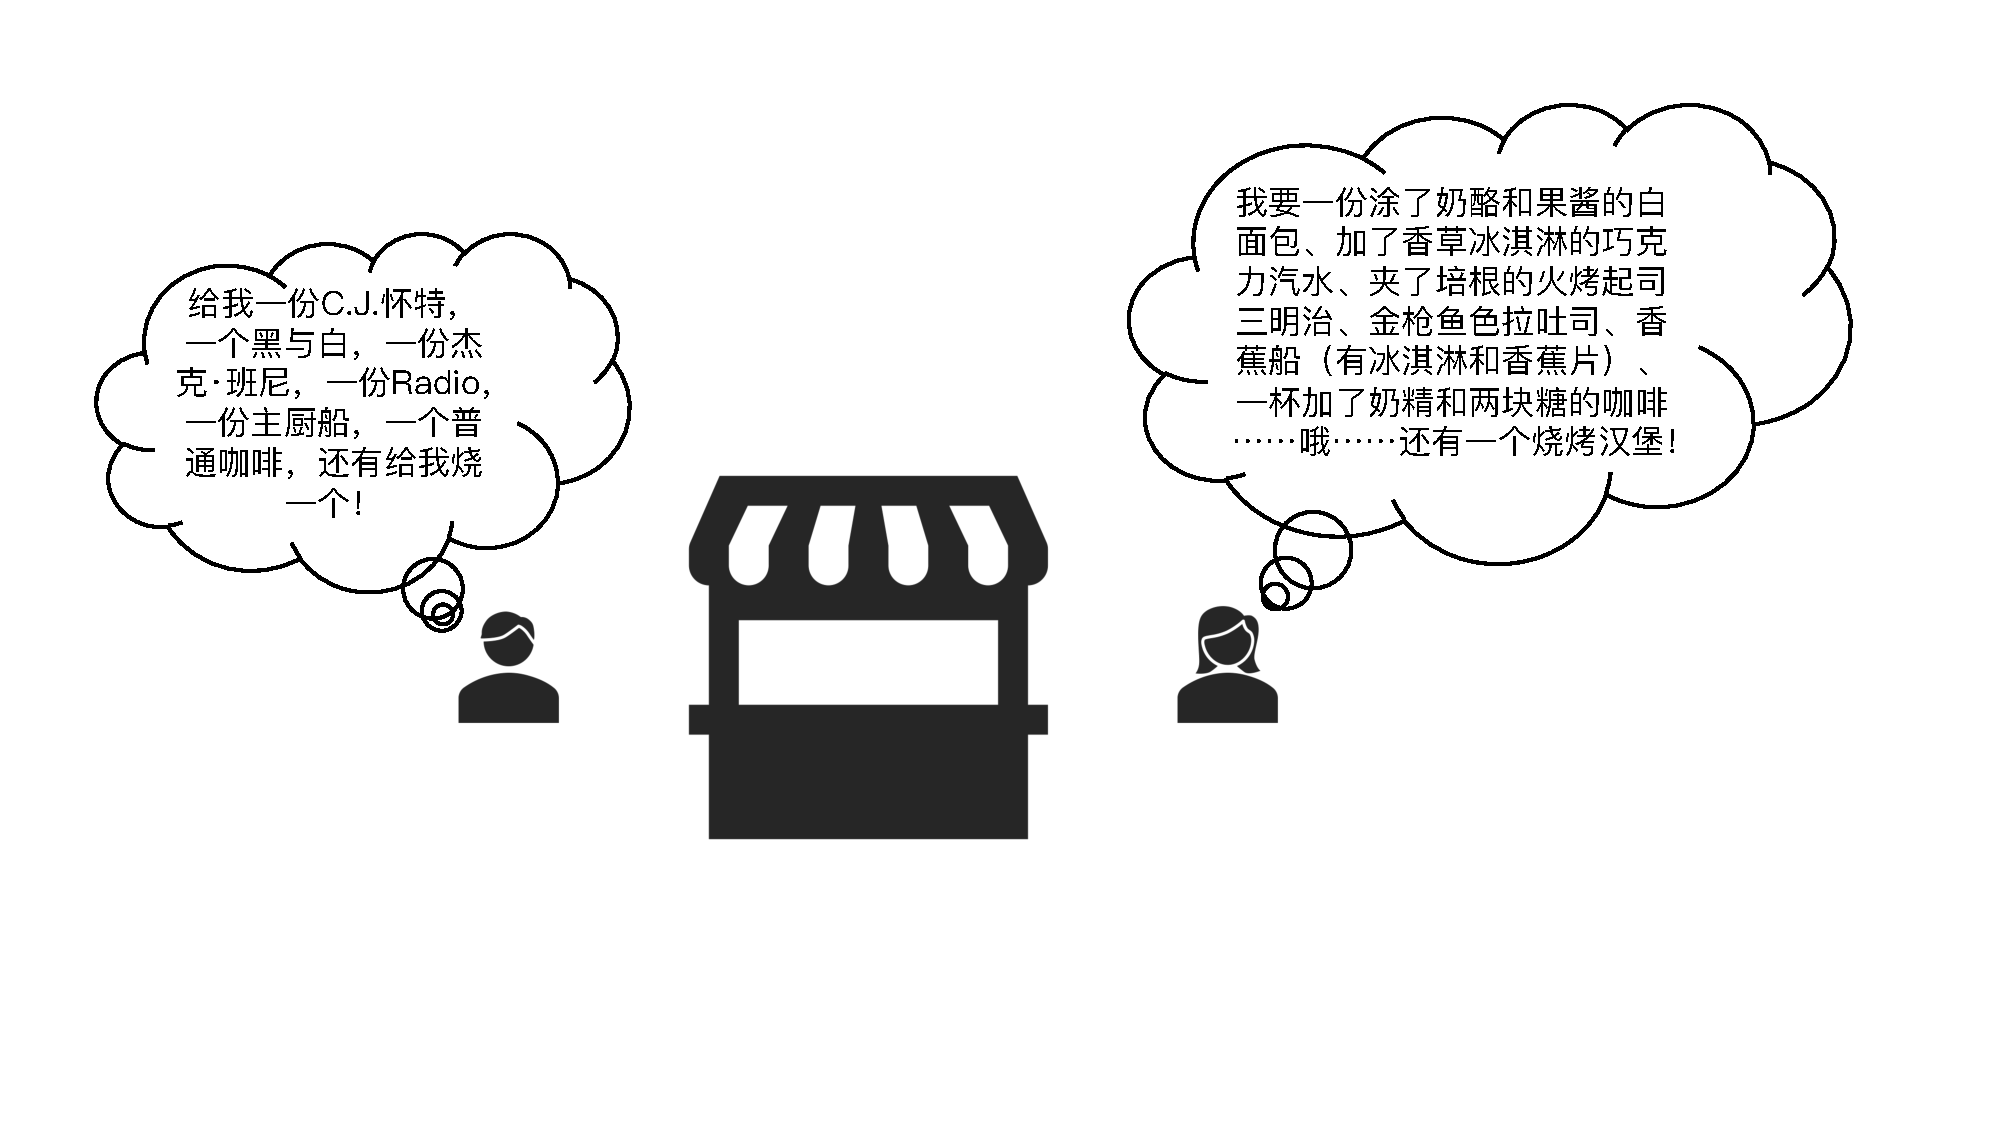
\includegraphics[width=0.8\textwidth]{images/共享词汇.pdf}
    \vspace{-1em}
\end{figure}

\subsubsection{共享模式词汇的力量}
\begin{itemize}
    \item \textbf{共享的模式词汇“威力强大”。}当你使用模式名称和其他开发人员或者开发团队沟通时,你们之间交流的不只是模式名称,而是一整套模式背后所象征的质量、特性、约束。
    \item \textbf{模式能够让你用更少的词汇做更充分的沟通。}当你用模式描述的时候,其他开发人员便很容易地知道你对设计的想法。
    \item \textbf{将说话的方式保持在模式层次,可让你待在“设计圈子”久一点。}使用模式谈论软件系统,可以让你保持在设计层次,不会被压低到对象与类这种琐碎的事情上面。
    \item \textbf{共享词汇可帮你的开发团队快速充电。}对于设计模式有深入了解的团队,彼此之间对于设计的看法不容易产生误解。
    \item \textbf{共享词汇能帮助初級开发人员迅速成长。}初级开发人员向有经验的开发人员看齐。当高级开发人员使用设计模式,初级开发人员也会跟着学。把你的组织建立成一个模式使用者的社区。
\end{itemize}

\subsection{库与设计模式}
\begin{figure}[H]
    \vspace{-0.5em}
	\centering
	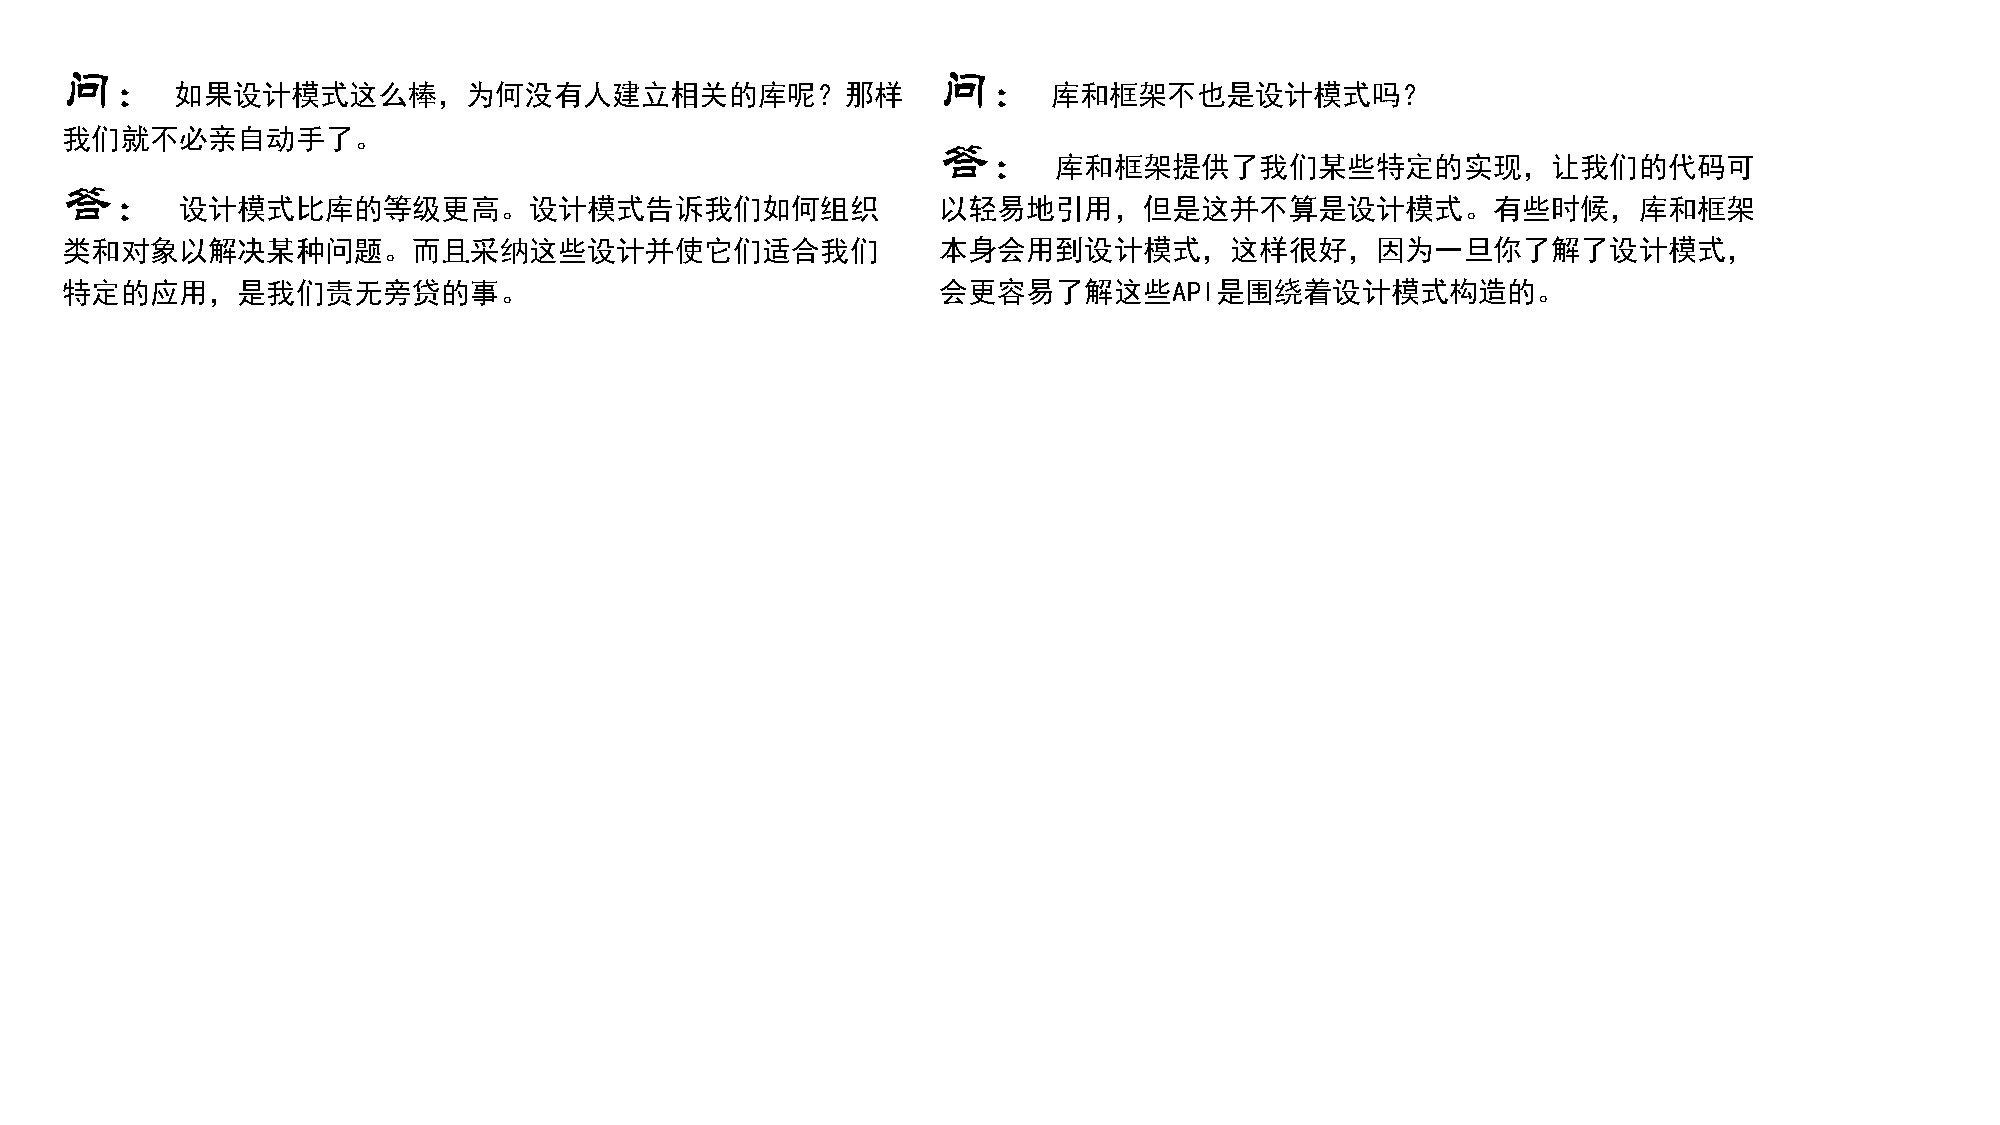
\includegraphics[width=\textwidth]{images/库与设计模式.pdf}
    \vspace{-1em}
\end{figure}

\subsection{要点总结}
\begin{itemize}
    \item 知道OO基础,井不足以让你设计出良好的OO系统。
    \item 良好的OO设计必须具备可复用、可扩充、可维护三个特性。
    \item 模式可以让我们建造出具有良好OO设计质量的系统。
    \item 模式被认为是历经验证的OO设计经验。
    \item 模式不是代码,而是针对设计问题的通用解决方案。你可把它们应用到特定的应用中。
    \item 模式不是被发明,而是被发现。
    \item 大多数的模式和原则,都着眼于软件变化的主题。
    \item 大多数的模式都允许系统局部改变独立于其他部分。
    \item 我们常把系统中会变化的部分抽出来封装。
    \item 模式让开发人员之间有共享的语言,能够最大化沟通的价值。
\end{itemize}





	\section{面向对象设计原则}

\subsection{面向对象设计原则概述}

\subsubsection{软件的可维护性和重用性}
知名软件大师Robert C.Martin认为一个可维护性(Maintainability)较低的软件设计,通常由于如下4个原因造成:
\vspace{-0.8em}
\begin{multicols}{2}
    \begin{itemize}
        \item 过于僵硬(Rigidity)
        \item 过于脆弱(Fragility)
        \item 复用率低(Immobility)
        \item 黏度过高(Viscosity)
    \end{itemize}
    \end{multicols}
\vspace{-1em}

软件工程和建模大师Peter Coad认为,一个好的系统设计应该具备如下三个性质:
\vspace{-0.8em}
\begin{multicols}{3}
    \begin{itemize}
        \item 可扩展性(Extensibility)
        \item 灵活性(Flexibility)
        \item 可插入性(Pluggability)
    \end{itemize}
    \end{multicols}
\vspace{-1em}

软件的可维护性和可复用性
\begin{itemize}
    \item 软件的\textbf{复用}(Reuse)或\textbf{重用}拥有众多优点,如可以提高软件的开发效率,提高软件质量,节约开发成本,\textbf{恰当的复用还可以改善系统的可维护性}。
    \item 面向对象设计复用的目标在于\textbf{实现支持可维护性的复用}。 
    \item 在面向对象的设计里面,\textbf{可维护性复用都是以面向对象设计原则为基础的},这些设计原则首先都是复用的原则,遵循这些设计原则可以有效地提高系统的复用性,同时提高系统的可维护性。
    \item 面向对象设计原则也是对系统进行合理重构的指南针,\textbf{重构} (Refactoring)是在不改变软件现有功能的基础上,通过调整程序代码改善软件的质量、性能,使其程序的设计模式和架构更趋合理,提高软件的扩展性和维护性。
\end{itemize}

\subsubsection{面向对象设计原则}
常用的面向对象设计原则包括7个,这些原则并不是孤立存在的,它们相互依赖,相互补充。
\vspace{-0.5em}
\begin{spacing}{1.2}
    \centering
    \begin{longtable}{|W{c}{6cm}|m{6.8cm}|W{c}{1.5cm}|}
        \hline
        设计原则名称    & \multicolumn{1}{c|}{设计原则简介}     & 重要性   \\ \hline
        \begin{tabular}[c]{@{}c@{}}单一职责原则\\ (Single Responsibility Principle, SRP)\end{tabular} & 类的职责要单一,不能将太多的职责放在一个类中                                                      & \ding{72}\ding{72}\ding{72}\ding{72}\ding{73} \\ \hline
        \begin{tabular}[c]{@{}c@{}}开闭原则\\ (Open-Closed Principle, OCP)\end{tabular}             & 软件实体对扩展是开放的,但对修改是关闭的,即在不修改一个软件实体的基础上去扩展其功能                                 & \ding{72}\ding{72}\ding{72}\ding{72}\ding{72} \\ \hline
        \begin{tabular}[c]{@{}c@{}}里氏代换原则\\ (Liskov Substitution Principle, LSP)\end{tabular}   & 在软件系统中,一个可以接受基类对象的地方必然可以接受一 个子类对象                                           & \ding{72}\ding{72}\ding{72}\ding{72}\ding{73} \\ \hline
        \begin{tabular}[c]{@{}c@{}}依赖倒转原则\\ (Dependency Inversion Principle, DIP)\end{tabular}  & 要针对抽象层编程,而不要针对具体类编程                                                         & \ding{72}\ding{72}\ding{72}\ding{72}\ding{72} \\ \hline
        \begin{tabular}[c]{@{}c@{}}接口隔离原则\\ (Interface Segregation Principle, ISP)\end{tabular} & 使用多个专门的接口来取代一个统一的接口                                                         & \ding{72}\ding{72}\ding{73}\ding{73}\ding{73} \\ \hline
        \begin{tabular}[c]{@{}c@{}}合成复用原则\\ (Composite Reuse Principle, CRP)\end{tabular}       & 在系统中应该尽量多使用组合和聚合关联关系,尽量少使用甚至不使用继承关系                                        & \ding{72}\ding{72}\ding{72}\ding{72}\ding{73} \\ \hline
        \begin{tabular}[c]{@{}c@{}}迪米特法则\\ (Law of Demeter, LoD)\end{tabular}                   & 一个软件实体对其他实体的引用越少越好,或者说如果两个类 不必彼此直接通信,那么这两个类就不应当发生直接的相互作用,而是通过引入一个第三者发生间接交互 & \ding{72}\ding{72}\ding{72}\ding{73}\ding{73} \\ \hline
    \end{longtable}
\end{spacing}
\vspace{-1em}

\subsection{单一职责原则}

\subsubsection{单一职责原则定义}
单一职责原则(Single Responsibility Principle, SRP)定义为:\textbf{一个对象应该只包含单一的职责,并且该职责被完整地封装在一个类中}。Every object should have a single responsibility, and that responsibility should be entirely encapsulated by the class.

另一种定义方式为:\textbf{就一个类而言,应该仅有一个引起它变化的原因}。There should never be more than one reason for a class to change.

\subsubsection{单一职责原则分析}
\begin{itemize}
    \item 一个类(或者大到模块,小到方法)\textbf{承担的职责越多,它被复用的可能性越小},而且如果一个类承担的职责过多,就相当于将这些职责耦合在一起,当其中一个职责变化时,可能会影响其他职责的运作。
    \item 类的职责主要包括两个方面:数据职责和行为职责,数据职责通过其属性来体现,而行为职责通过其方法来体现。
    \item 单一职责原则是实现\textbf{高内聚、低耦合}的指导方针,在很多代码重构手法中都能找到它的存在,它是最简单但又最难运用的原则,需要设计人员发现类的不同职责并将其分离,而发现类的多重职责需要设计人员具有较强的分析设计能力和相关重构经验。
\end{itemize}

\subsubsection{单一职责原则实例}
某基于Java的C/S系统的“登录功能”通过如下登录类(Login)实现
\begin{figure}[H]
    \vspace{-0.5em}
	\centering
	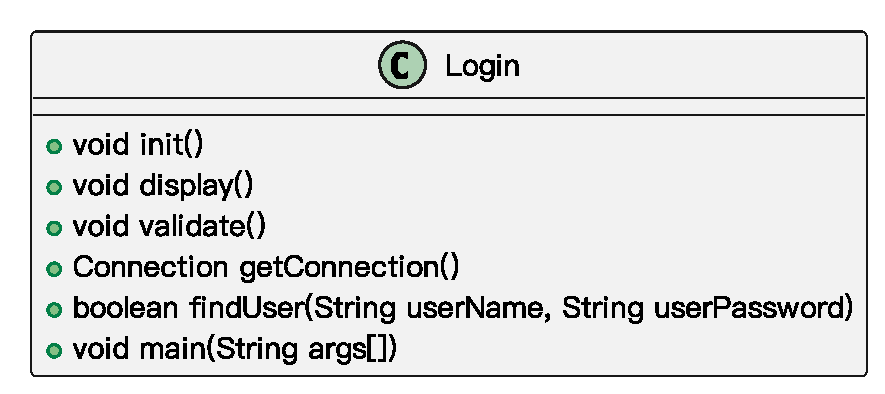
\includegraphics[width=0.55\textwidth]{images/单一职责原则实例1.eps}
    \vspace{-1em}
\end{figure}

使用单一职责原则对其进行重构如下
\begin{figure}[H]
    \vspace{-0.5em}
	\centering
	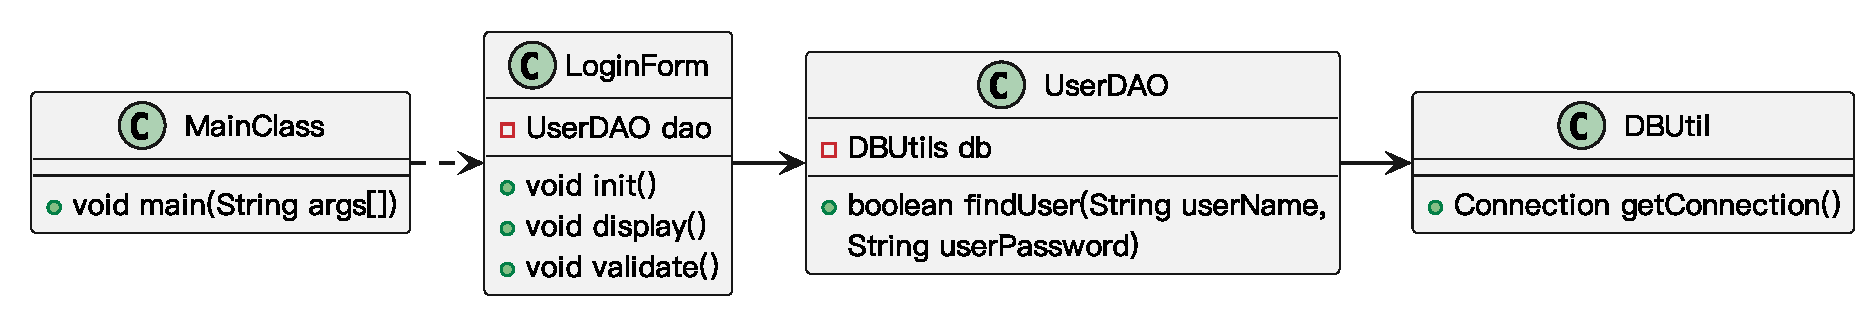
\includegraphics[width=\textwidth]{images/单一职责原则实例2.eps}
    \vspace{-1em}
\end{figure}

\subsection{开闭原则}

\subsubsection{开闭原则定义}
开闭原则(Open-Closed Principle, OCP)定义为:一个软件实体应当\textbf{对扩展开放,对修改关闭}。也就是说在设计一个模块的时候,应当使这个模块可以在不被修改的前提下被扩展,即实现在不修改源代码的情况下改变这个模块的行为。Software entities should be open for extension, but closed for modification.

\subsubsection{开闭原则分析}
\begin{itemize}
    \item 开闭原则由Bertrand Meyer于1988年提出,它是面向对象设计中最重要的原则之一。
    \item 在开闭原则的定义中,软件实体可以指一个软件模块、一个由多个类组成的局部结构或一个独立的类。
    \item \textbf{抽象化}是开闭原则的关键。
    \item 开闭原则还可以通过一个更加具体的“\textbf{对可变性封装原则}”来描述,对可变性封装原则(Principle of Encapsulation of Variation, EVP)要求找到系统的可变因素并将其封装起来。
\end{itemize}

\subsubsection{开闭原则实例}
某图形界面系统提供了各种不同形状的按钮,客户端代码可针对这些按钮进行编程,用户可能会改变需求要求使用不同的按钮,原始设计方案如图所示
\begin{figure}[H]
    \vspace{-0.5em}
	\centering
	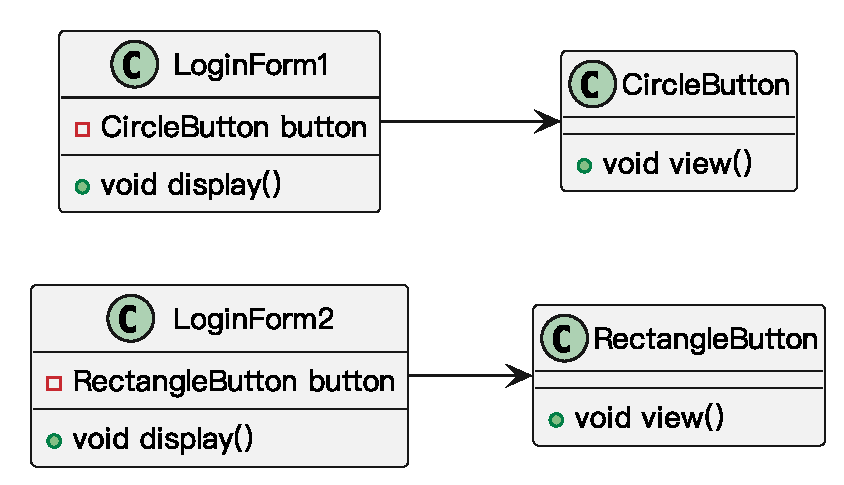
\includegraphics[width=0.5\textwidth]{images/开闭原则实例1.eps}
    \vspace{-1em}
\end{figure}

现对该系统进行重构,使之满足开闭原则的要求:尝试将代码变为数据(配置文件\;\verb|config.xml|)结合Java的反射机制完成
\begin{figure}[H]
    \vspace{-0.5em}
	\centering
	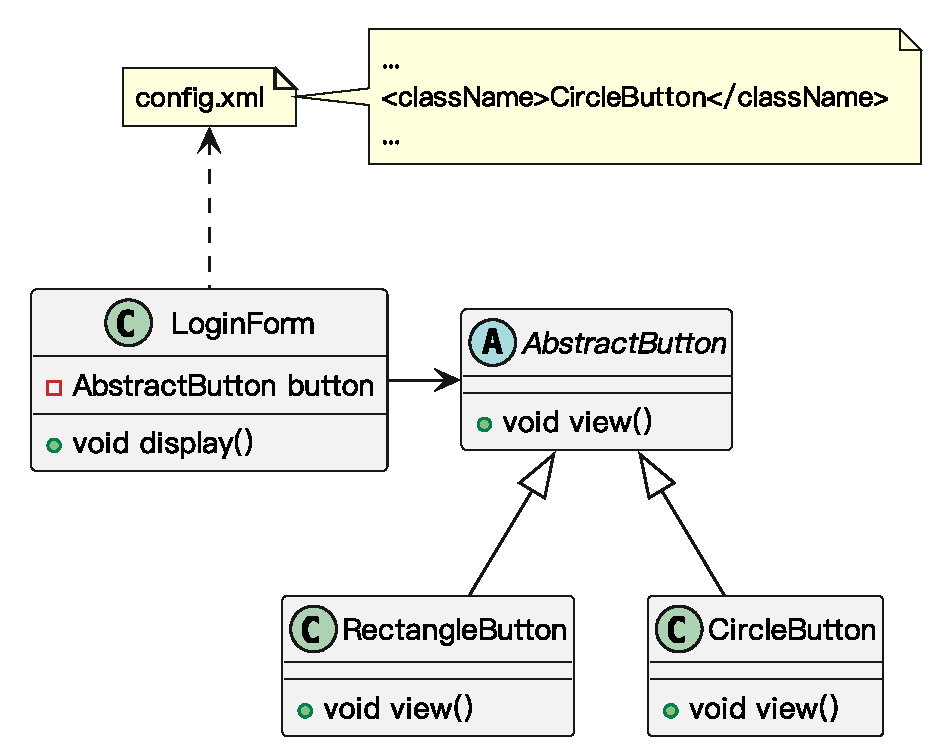
\includegraphics[width=0.55\textwidth]{images/开闭原则实例2.eps}
    \vspace{-1em}
\end{figure}

\subsection{里氏代换原则}

\subsubsection{里氏代换原则定义}
里氏代换原则(Liskov Substitution Principle, LSP)有两种定义方式,第一种定义方式相对严格,其定义为:
如果对每一个类型为$S$的对象$O_1$,都有类型为$T$的对象$O_2$,使得以$T$定义的所有程序$P$在所有的对象$O_2$都代换成$O_1$时,程序$P$的行为没有变化,那么类型$S$是类型$T$的子类型。If for each object $O_1$ of type $S$ there is an object $O_2$ of type $T$ such that for all programs $P$ defined in terms of $T$, the behavior of $P$ is unchanged when $O_1$ is substituted for $O_2$ then $S$ is a subtype of $T$.

第二种更容易理解的定义方式为:\textbf{所有引用基类(父类)的地方必须能透明地使用其子类的对象}。Functions that use pointers or references to base classes must be able to use objects of derived classes without knowing it.

\subsubsection{里氏代换原则分析}
\begin{itemize}
    \item 里氏代换原则由2008年图灵奖得主、美国第一位计算机科学女博士、麻省理工学院教授Barbara Liskov和卡内基·梅隆大学Jeannette Wing教授于1994年提出。
    \item 里氏代换原则可以通俗表述为:\textbf{在软件中如果能够使用基类对象,那么一定能够使用其子类对象}。把基类都替换成它的子类,程序将不会产生任何错误和异常,反过来则不成立,如果一个软件实体使用的是一个子类的话,那么它不一定能够使用基类。
    \item 里氏代换原则是实现开闭原则的重要方式之一,由于使用基类对象的地方都可以使用子类对象,因此\textbf{在程序中尽量使用基类类型来对对象进行定义,而在运行时再确定其子类类型,用子类对象来替换父类对象}。
\end{itemize}

\subsubsection{里氏代换原则实例}
某系统需要实现对重要数据(如用户密码)的加密处理,在数据操作类(\verb|DataOperator|)中需要调用加密类中定义的加密算法,系统提供了两个不同的加密类\;\verb|CipherA|\;和\;\verb|CipherB|,它们实现不同的加密方法,在\;\verb|DataOperator|\;中可以选择其中的一个实现加密操作。
\begin{figure}[H]
    \vspace{-0.5em}
	\centering
	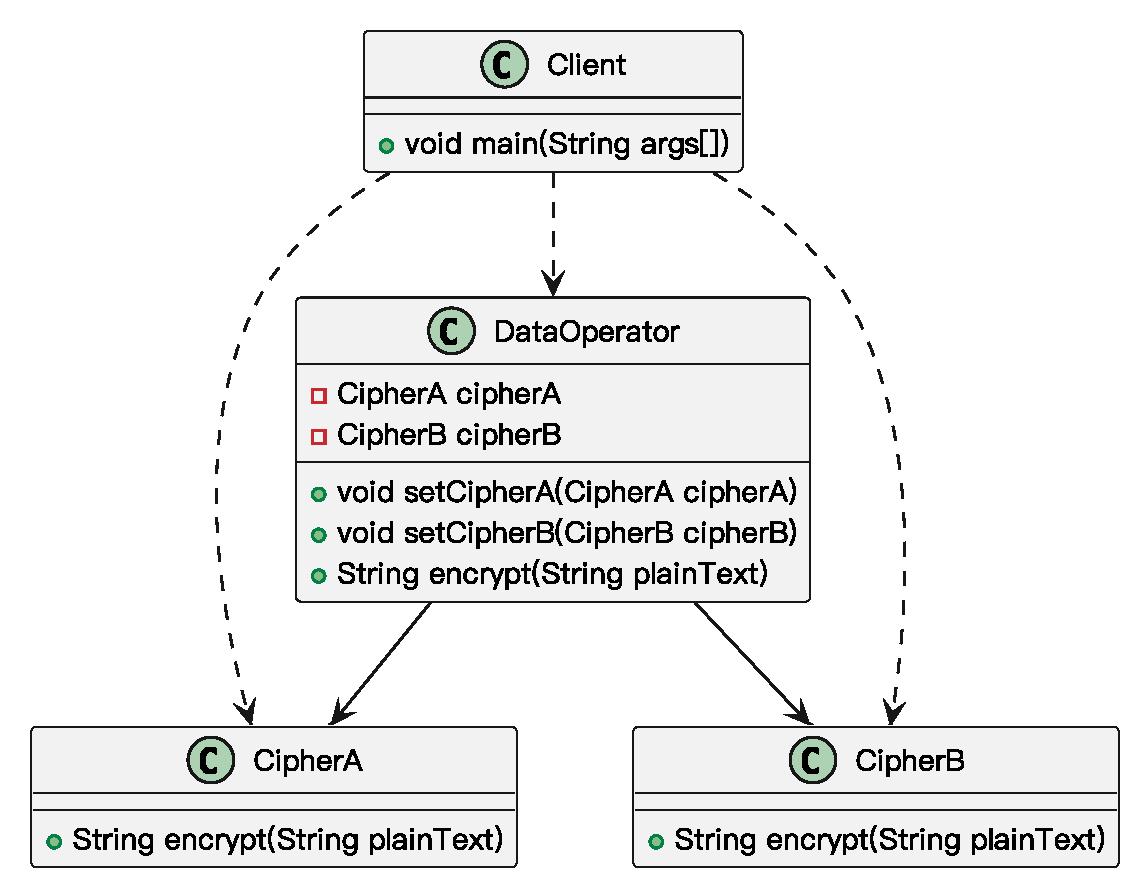
\includegraphics[width=0.6\textwidth]{images/里氏代换原则实例1.eps}
    \vspace{-1em}
\end{figure}

也可以为\;\verb|CipherA|\;和\;\verb|CipherB|\;设计一个共同的父类,下面是指\;\verb|CipherB|\;是在\;\verb|CipherA|\;的基础上加密。
\begin{figure}[H]
    \vspace{-0.5em}
	\centering
	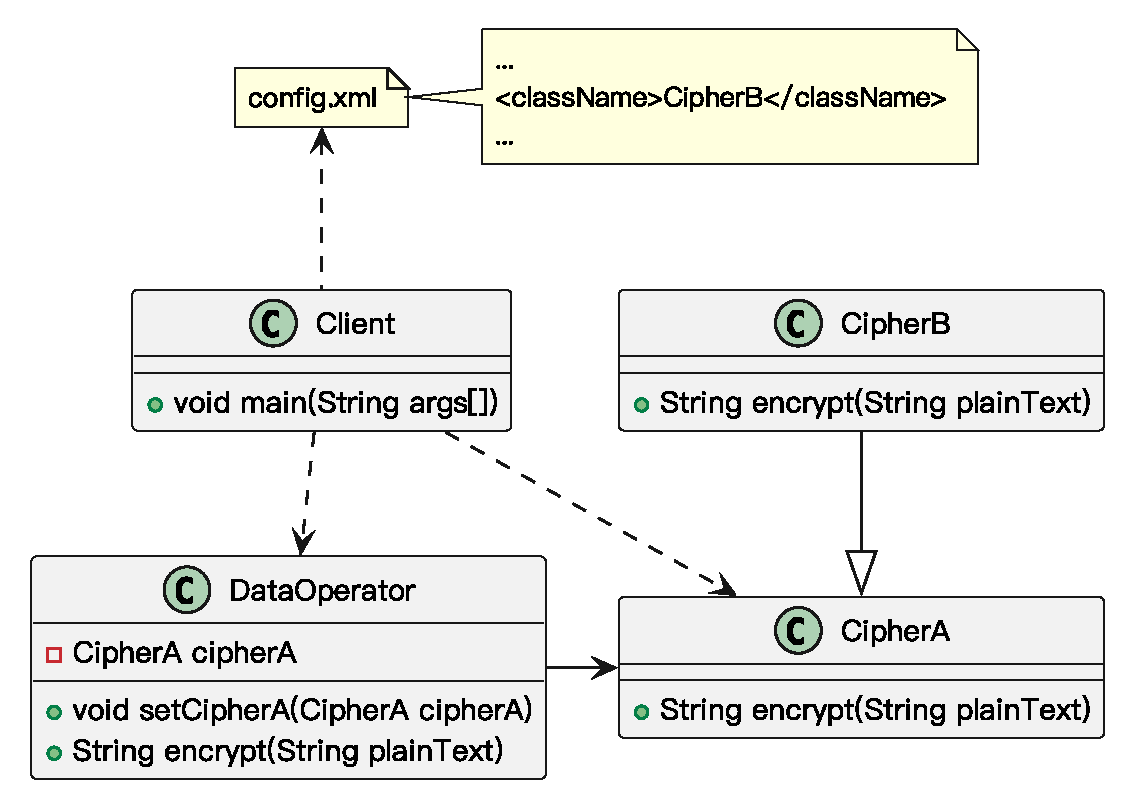
\includegraphics[width=0.65\textwidth]{images/里氏代换原则实例2.eps}
    \vspace{-1em}
\end{figure}

\subsection{依赖倒转原则}

\subsubsection{依赖倒转原则定义}
依赖倒转原则(Dependence Inversion Principle, DIP)的定义为:\textbf{高层模块不应该依赖低层模块,它们都应该依赖抽象。抽象不应该依赖于细节,细节应该依赖于抽象。}High level modules should not depend upon low level modules, both should depend upon abstractions. Abstractions should not depend upon details, details should depend upon abstractions.

另一种表述为:\textbf{要针对接口编程,不要针对实现编程}。Program to an interface, not an implementation.

\subsubsection{依赖倒转原则分析}
\begin{itemize}
    \item 简单来说,依赖倒转原则就是指:\textbf{代码要依赖于抽象的类,而不要依赖于具体的类;要针对接口或抽象类编程,而不是针对具体类编程}。
    \item 实现开闭原则的关键是抽象化,并且从抽象化导出具体化实现,如果说\textbf{开闭原则是面向对象设计的目标的话},那么\textbf{依赖倒转原则就是面向对象设计的主要手段}。
    \item 依赖倒转原则的常用实现方式之一是在代码中使用抽象类,而将具体类放在配置文件:\textbf{将抽象放进代码,将细节放进元数据}。
\end{itemize}

类之间的耦合关系有零耦合关系、具体耦合关系和抽象耦合关系
\begin{itemize}
    \item 零耦合关系:两个类没有依赖关系
    \item 具体耦合关系:两个具体的类之间有依赖关系,表现为一个具体类直接引用另外一个具体类
    \item 抽象耦合关系:发生在一个具体类和一个抽象类之间,这样就使必须发生关系的类之间保持最大的灵活性
\end{itemize}

依赖倒转原则要求客户端依赖于抽象耦合,\textbf{以抽象方式耦合是依赖倒转原则的关键}。

\subsubsection{依赖倒转原则实例}
某系统提供一个数据转换模块,可以将来自不同数据源的数据转换成多种格式,如可以转换来自数据库的数据(\verb|DatabaseSource|)、也可以转换来自文本文件的数据(\verb|TextSource|),转换后的格式可以是XML文件(\verb|XMLTransformer|)、也可以是XLS文件(\verb|XLSTransformer|)等。
\begin{figure}[H]
    \vspace{-0.5em}
	\centering
	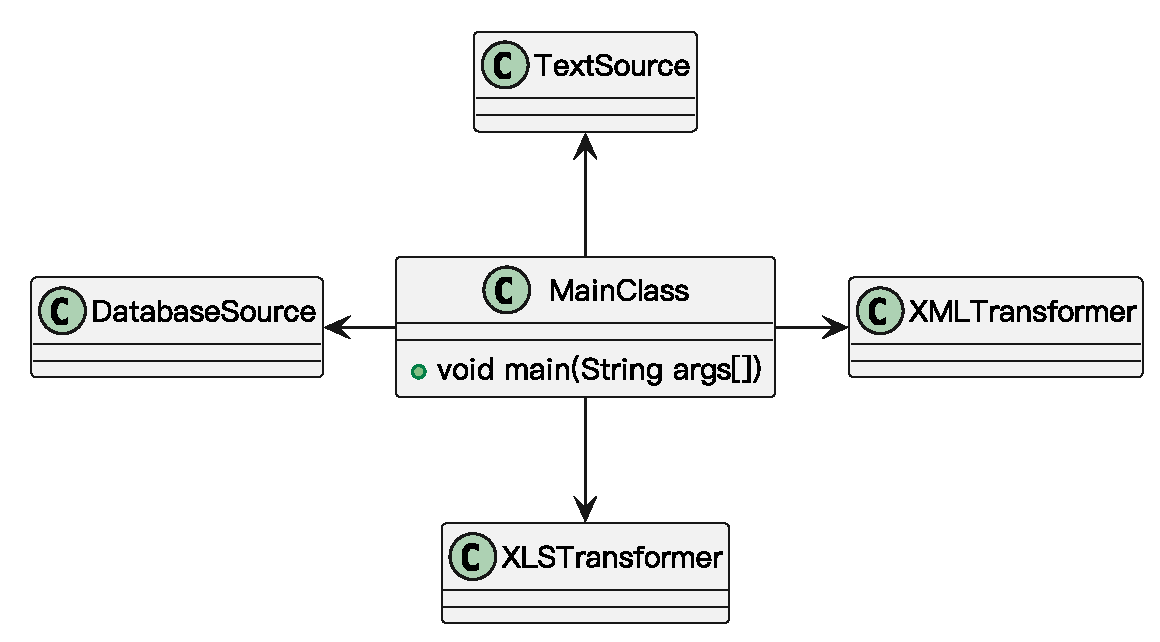
\includegraphics[width=0.55\textwidth]{images/依赖倒转原则实例1.eps}
    \vspace{-1em}
\end{figure}

由于需求的变化,该系统可能需要增加新的数据源或者新的文件格式,每增加一个新的类型的数据源或者新的类型的文件格式,客户类\;\verb|MainClass|\;都需要修改源代码,以便使用新的类,但违背了开闭原则。现使用依赖倒转原则对其进行重构。
\begin{figure}[H]
    \vspace{-0.5em}
	\centering
	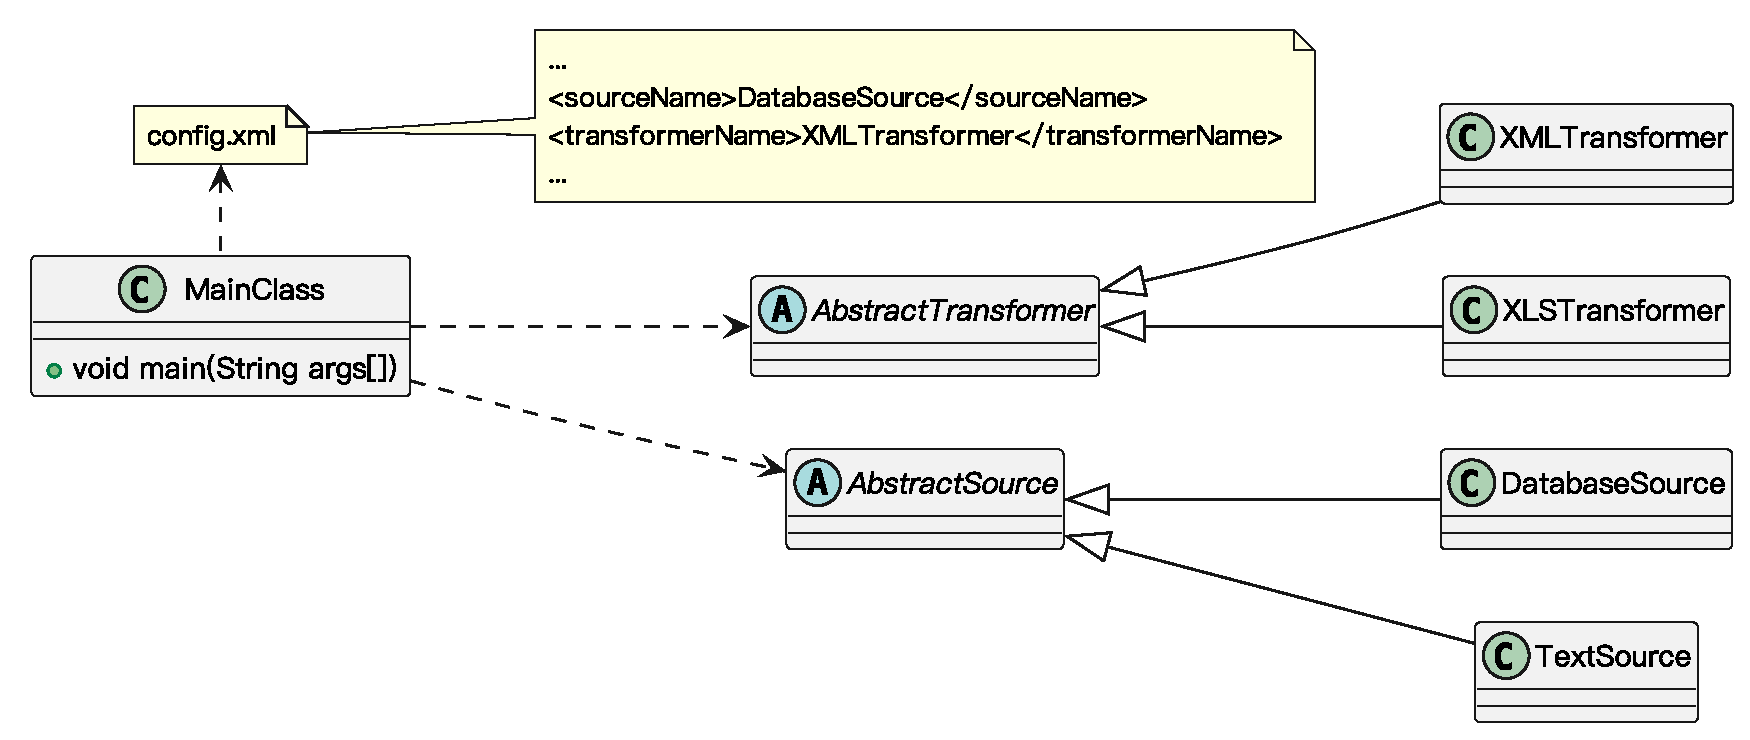
\includegraphics[width=0.9\textwidth]{images/依赖倒转原则实例2.eps}
    \vspace{-1em}
\end{figure}

\subsection{接口隔离原则}

\subsubsection{接口隔离原则定义}
接口隔离原则(Interface Segregation Principle, ISP)的定义为:\textbf{客户端不应该依赖那些它不需要的接口}。Clients should not be forced to depend upon interfaces that they do not use.
\begin{itemize}
    \item 在该定义中的接口指的是所定义的方法。
\end{itemize}

另一种定义方法如下:\textbf{一旦一个接口太大,则需要将它分割成一些更细小的接口},使用该接口的客户端仅需知道与之相关的方法即可。Once an interface has gotten too fat it needs to be split into smaller and more specific interfaces so that any clients of the interface will only know about the methods that pertain to them.

\subsubsection{接口隔离原则分析}
\begin{itemize}
    \item 接口隔离原则是指\textbf{使用多个专门的接口,而不使用单一的总接口}。每一个接口应该承担一种相对独立的角色,不多不少,不干不该干的事,该干的事都要干。
    \begin{itemize}
        \item 一个接口就\textbf{只代表一个角色},每个角色都有它特定的一个接口,此时这个原则可以叫做“角色隔离原则”。
        \item 接口\textbf{仅仅提供客户端需要的行为},即所需的方法,客户端不需要的行为则隐藏起来,应当为客户端提供尽可能小的单独的接口,而不要提供大的总接口。
    \end{itemize}
    \item 使用接口隔离原则拆分接口时,\textbf{首先必须满足单一职责原则},将一组相关的操作定义在一个接口中,且在满足高内聚的前提下,接口中的方法越少越好。
    \item 可以在进行系统设计时采用\textbf{定制服务}的方式,即\textbf{为不同的客户端提供宽窄不同的接口},只提供用户需要的行为,而隐藏用户不需要的行为。
\end{itemize}

\subsubsection{接口隔离原则实例}
下图展示了一个拥有多个客户类的系统,在系统中定义了一个巨大的接口(胖接口)\verb|AbstractService|\;来服务所有的客户类。
\begin{figure}[H]
    \vspace{-0.5em}
	\centering
	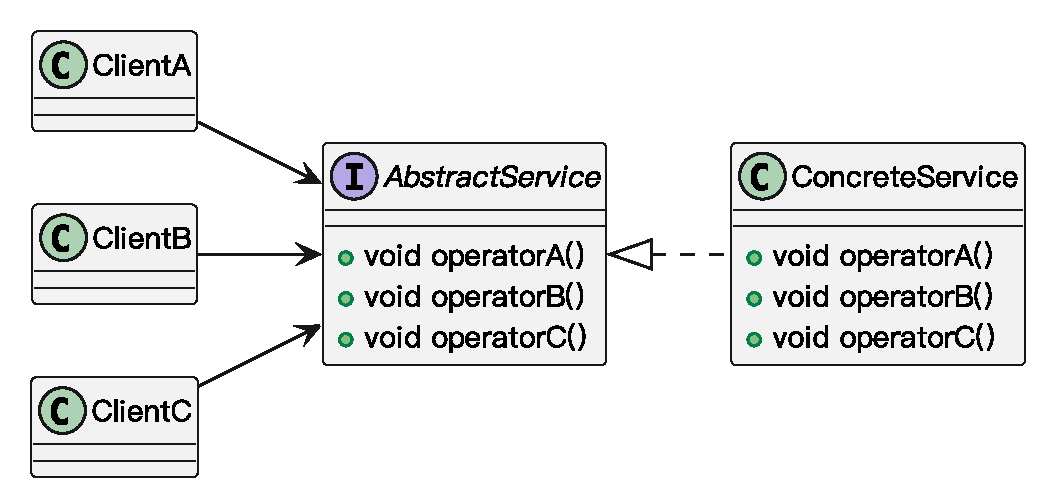
\includegraphics[width=0.6\textwidth]{images/接口隔离原则实例1.eps}
    \vspace{-1em}
\end{figure}

使用接口隔离原则对其进行重构如下。
\begin{figure}[H]
    \vspace{-0.5em}
	\centering
	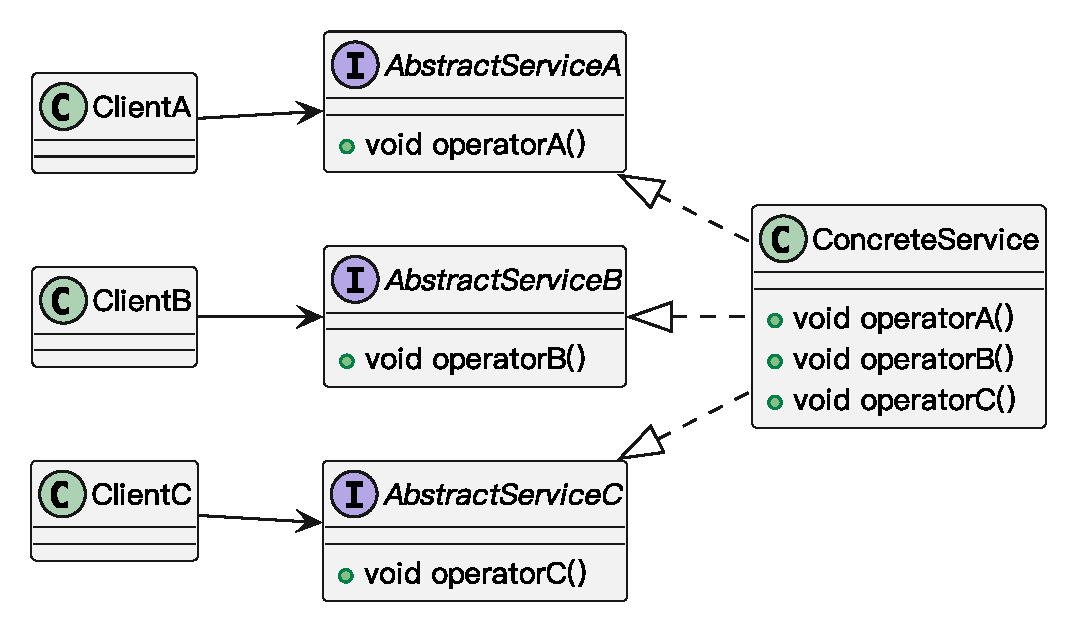
\includegraphics[width=0.6\textwidth]{images/接口隔离原则实例2.eps}
    \vspace{-1em}
\end{figure}

\subsection{合成复用原则}

\subsubsection{合成复用原则定义}
合成复用原则(Composite Reuse Principle, CRP)又称为组合/聚合复用原则(Composition/ Aggregate Reuse Principle, CARP),其定义为:\textbf{尽量使用对象组合,而不是继承来达到复用的目的}。Favor composition of objects over inheritance as a reuse mechanism.

\subsubsection{合成复用原则分析}
在面向对象设计中,可以通过两种基本方法在不同的环境中复用已有的设计和实现,即通过组合/ 聚合关系或通过继承。
\begin{itemize}
    \item 继承复用:实现简单,易于扩展。破坏系统的封装性;从基类继承而来的实现是静态的,不可能在运行时发生改变,没有足够的灵活性;只能在有限的环境中使用。("白箱"复用)
    \item 组合/聚合复用:耦合度相对较低,选择性地调用成员对象的操作;可以在运行时动态进行。("黑箱"复用)
\end{itemize}

合成复用原则就是指在一个新的对象里通过关联关系(包括组合关系和聚合关系)来使用一些已有的对象,使之成为新对象的一部分;新对象通过委派调用已有对象的方法达到复用其已有功能的目的。简言之:\textbf{要尽量使用组合/聚合关系,少用继承}。

组合/聚合可以\textbf{使系统更加灵活},类与类之间的\textbf{耦合度降低},一个类的变化对其他类造成的影响相对较少,因此一般\textbf{首选使用组合/聚合来实现复用};其次才考虑继承,在使用继承时,需要严格遵循里氏代换原则,有效使用继承会有助于对问题的理解,降低复杂度,而滥用继承反而会增加系统构建和维护的难度以及系统的复杂度,因此需要\textbf{慎重使用继承复用}。

\subsubsection{合成复用原则实例}
某教学管理系统部分数据库访问类设计如图所示:
\begin{figure}[H]
    \vspace{-0.5em}
	\centering
	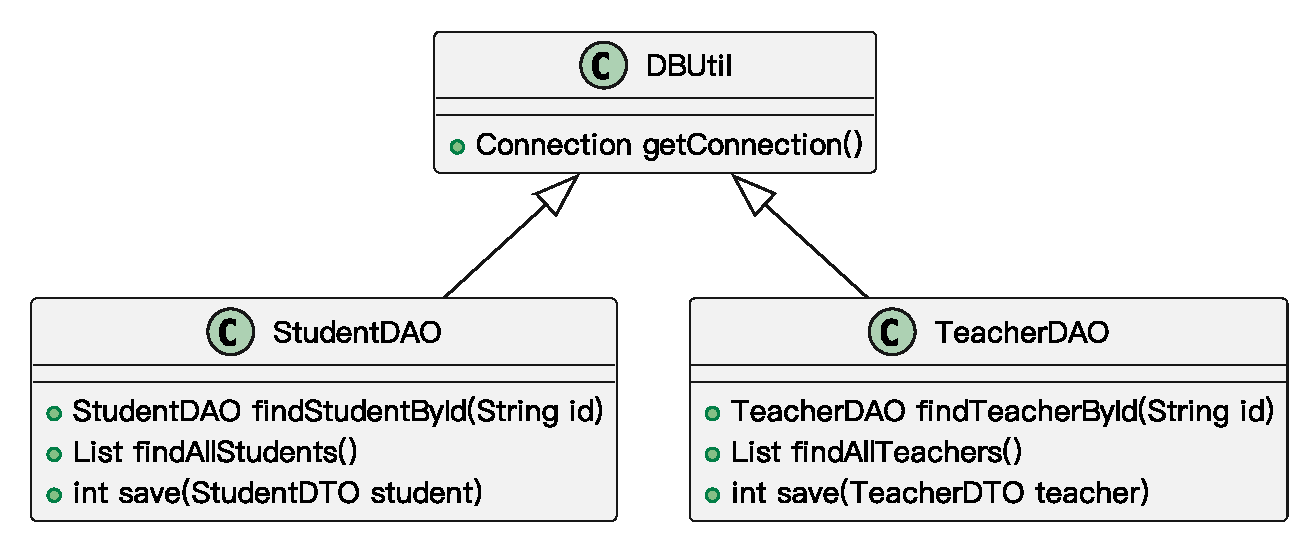
\includegraphics[width=0.7\textwidth]{images/合成复用原则实例1.eps}
    \vspace{-1em}
\end{figure}

如果需要更换数据库连接方式,如原来采用JDBC连接数据库,现在采用数据库连接池连接,则需要修改\;\verb|DBUtil|\;类源代码。如果\;\verb|StudentDAO|\;采用JDBC连接,但是\;\verb|TeacherDAO|\;采用连接池连接,则需要增加一个新的\;\verb|DBUtil|\;类,并修改\;\verb|StudentDAO|\;或\;\verb|TeacherDAO|\;的源代码,使之继承新的数据库连接类,这将违背开闭原则,系统扩展性较差。

现使用合成复用原则对其进行重构。
\begin{figure}[H]
    \vspace{-0.5em}
	\centering
	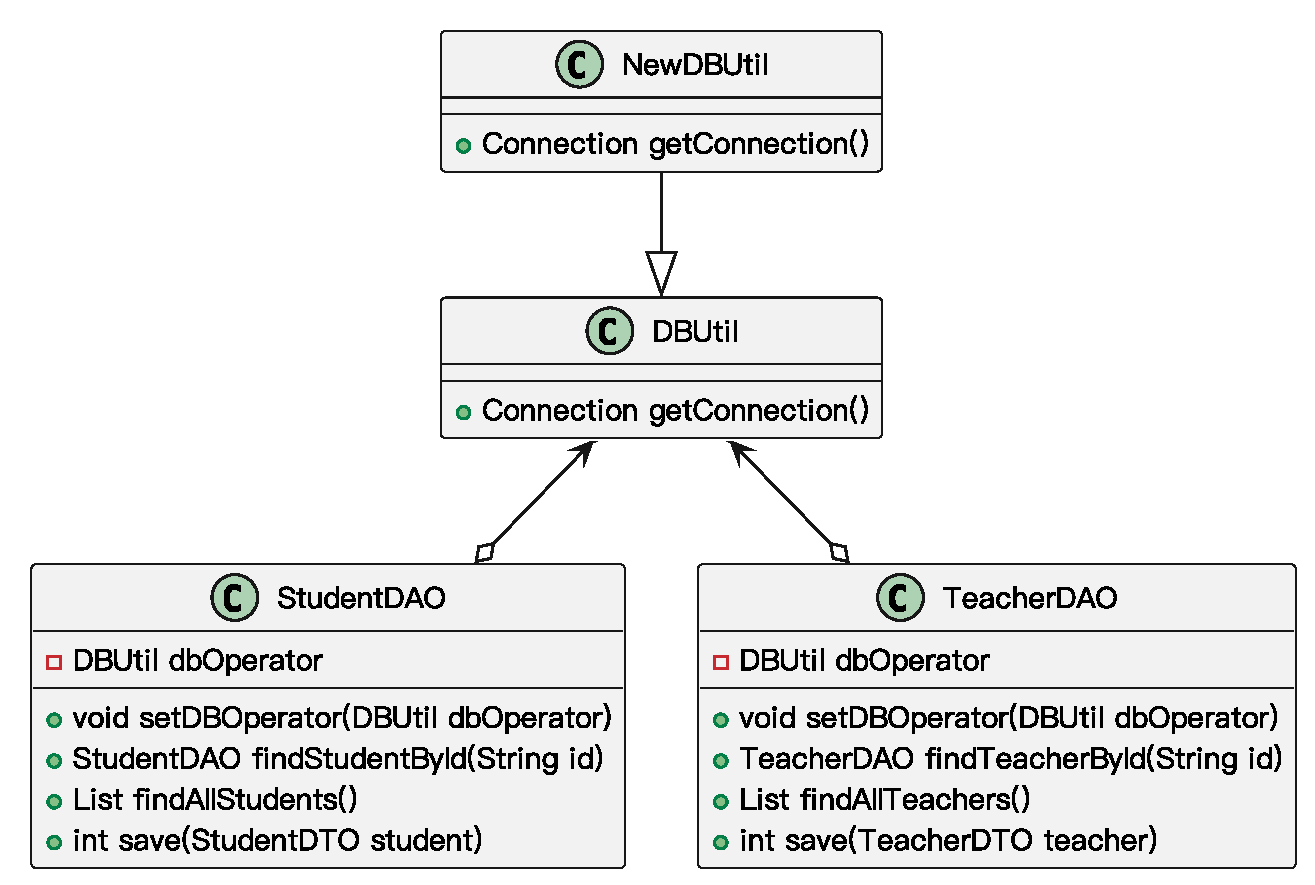
\includegraphics[width=0.75\textwidth]{images/合成复用原则实例2.eps}
    \vspace{-1em}
\end{figure}

\subsection{迪米特法则}

\subsubsection{迪米特法则定义}
迪米特法则(Law of Demeter, LoD)又称为最少知识原则(Least Knowledge Principle, LKP),它有多种定义方法,其中几种典型定义如下:
\begin{itemize}
    \item \textbf{不要和“陌生人”说话。}Don't talk to strangers.
    \item \textbf{只与你的直接朋友通信。}Talk only to your immediate friends.
    \item \textbf{每一个软件单位对其他的单位都只有最少的知识,而且局限于那些与本单位密切相关的软件单位。}Each unit should have only limited knowledge about other units: only units ``closely'' related to the current unit.
\end{itemize}

\subsubsection{迪米特法则分析}
\begin{itemize}
    \item 迪米特法则来自于1987年秋美国东北大学一个名为``Demeter''的研究项目。
    \item 简单地说,迪米特法则就是指\textbf{一个软件实体应当尽可能少的与其他实体发生相互作用}。这样,当一个模块修改时,就会尽量少的影响其他的模块,扩展会相对容易,这是对软件实体之间通信的限制,它要求限制软件实体之间通信的宽度和深度。
\end{itemize}

在迪米特法则中,对于一个对象,其“朋友”包括以下几类,若不满足如下条件中的一个,就是“陌生人”
\begin{enumerate}[label=(\arabic*)]
    \item 当前对象本身(this)
    \item 以参数形式传入到当前对象方法中的对象
    \item 当前对象的成员对象
    \item 如果当前对象的成员对象是一个集合,那么集合中的元素也都是朋友
    \item 当前对象所创建的对象
\end{enumerate}

迪米特法则可分为狭义法则和广义法则。\textbf{在狭义的迪米特法则中,如果两个类之间不必彼此直接通信,那么这两个类就不应当发生直接的相互作用},如果其中的一个类需要调用另一个类的某一个方法的话,可以\textbf{通过第三者转发这个调用}。
\begin{figure}[H]
    \vspace{-0.5em}
	\centering
	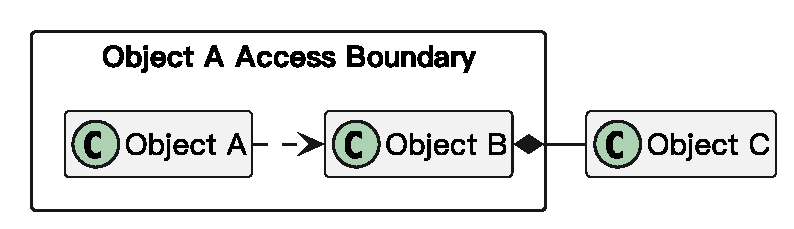
\includegraphics[width=0.45\textwidth]{images/狭义迪米特法则.eps}
    \vspace{-1em}
\end{figure}
\begin{itemize}
    \item 狭义的迪米特法则:可以降低类之间的耦合,但是会在系统中增加大量的小方法并散落在系统的各个角落,它可以使一个系统的局部设计简化,因为每一个局部都不会和远距离的对象有直接的关联,但是也会\textbf{造成系统的不同模块之间的通信效率降低},使得系统的不同模块之间不容易协调。
    \item 广义的迪米特法则:\textbf{指对对象之间的信息流量、流向以及信息的影响的控制},主要是\textbf{对信息隐藏的控制}。信息的隐藏可以使各个子系统之间脱耦,从而允许它们独立地被开发、优化、使用和修改,同时可以促进软件的复用,由于每一个模块都不依赖于其他模块而存在,因此每一个模块都可以独立地在其他的地方使用。一个系统的规模越大,信息的隐藏就越重要,而信息隐藏的重要性也就越明显。
\end{itemize}

迪米特法则的主要用途在于\textbf{控制信息的过载}:
\begin{itemize}
    \item 在类的划分上,应当尽量\textbf{创建松耦合的类},类之间的耦合度越低,就越有利于复用,一个处在松耦合中的类一旦被修改,不会对关联的类造成太大波及
    \item 在类的结构设计上,每一个类都应当\textbf{尽量降低其成员变量和成员函数的访问权限}
    \item 在类的设计上,只要有可能,\textbf{一个类型应当设计成不变类}
    \item 在对其他类的引用上,\textbf{一个对象对其他对象的引用应当降到最低}
\end{itemize}

\subsubsection{迪米特法则实例}
某系统界面类与数据访问类之间的调用关系较为复杂,如图所示:
\begin{figure}[H]
    \vspace{-0.5em}
	\centering
	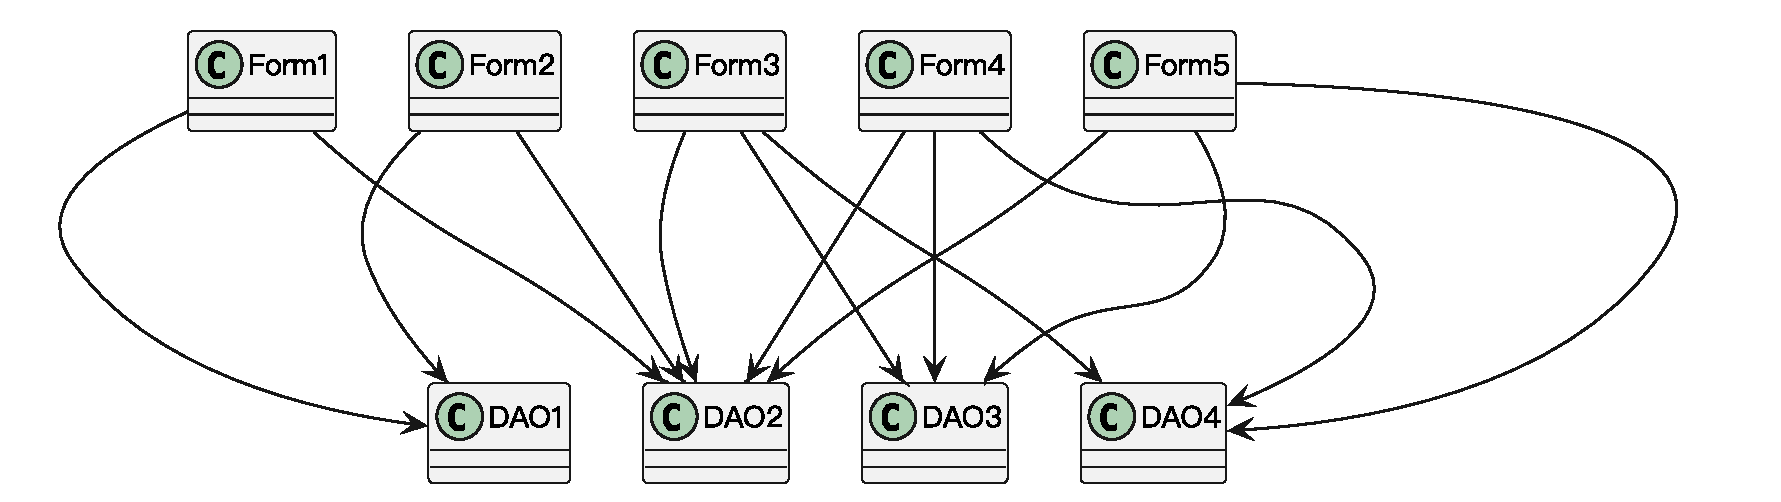
\includegraphics[width=0.85\textwidth]{images/迪米特法则实例1.eps}
    \vspace{-1em}
\end{figure}

修改如下
\begin{figure}[H]
    \vspace{-0.5em}
	\centering
	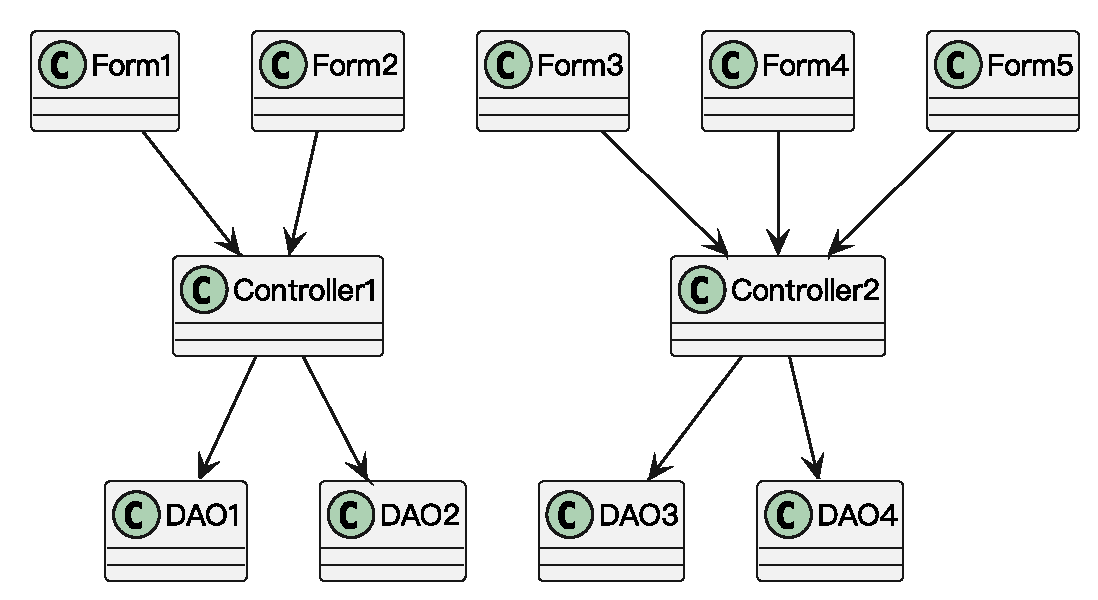
\includegraphics[width=0.55\textwidth]{images/迪米特法则实例2.eps}
    \vspace{-1em}
\end{figure}
	\section{策略模式}

\subsection{策略模式的引入}

\subsubsection{从模拟鸭子应用开始}
在模拟鸭子SimUDuck游戏中会出现各种鸭子,一边游泳戏水,一边呱呱叫。此系统的内部设计使用了标准的OO技术,设计了一个鸭子超类,并让各种鸭子继承此超类。
\begin{figure}[H]
    \vspace{-0.5em}
	\centering
	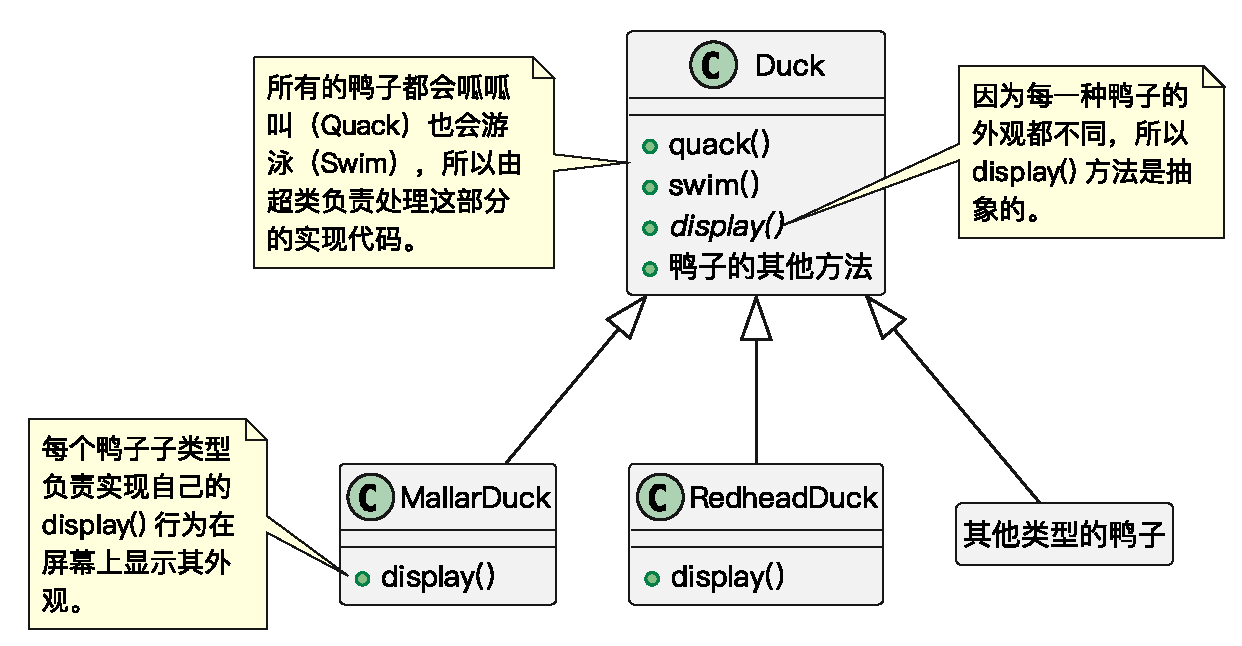
\includegraphics[width=0.75\textwidth]{images/SimUDuck1.eps}
    \vspace{-1em}
\end{figure}

现在需要添加功能使得鸭子可以飞。简单地修改鸭子父类,我们可以发现这样子橡皮鸭也可以飞,显然不是我们想要的。
\begin{itemize}
    \item 我们总是可以像使用\;\verb|quack()|\;方法一样在橡皮鸭中覆盖\;\verb|fly()|\;方法……
    \item 但是,当我们在程序中添加木制诱饵鸭子时会发生什么呢?他们不应该飞或嘎嘎……
    \item 高管们希望每六个月更新一次产品。每次更新中都会有新的\;\verb|Duck|\;子类,真是一场噩梦!
\end{itemize}

\begin{figure}[H]
    \vspace{-0.5em}
	\centering
	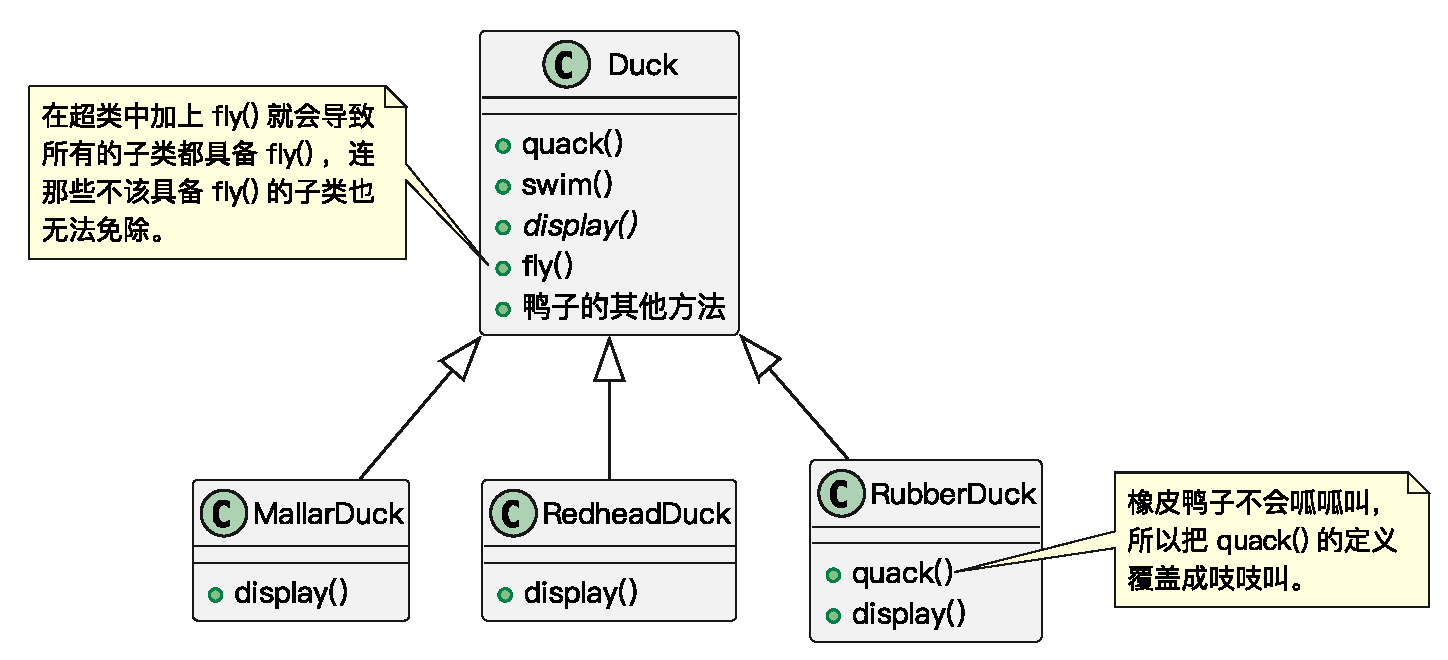
\includegraphics[width=0.75\textwidth]{images/SimUDuck2.eps}
    \vspace{-1em}
\end{figure}

我们知道,并非所有的子类都具有飞行和呱呱叫的行为,所以继承并不是适当的解决方式。那么使用接口会如何呢?

虽然\;\verb|Flyable|\;与\;\verb|Quackable|\;可以解決一部分问题(不会再有会飞的橡皮鸭),但是Java接口不具有实现代码,所以继承接口无法达到代码的复用,这意味着无论何时你需要修改某个行为,你必须得往下追踪并在每一个定义此行为的类中修改它,一不小心,可能会造成新的错误!这只能算是从一个恶梦跳进另一个恶梦。甚至,在会飞的鸭子中,飞行的动作可能还有多种变化……

\begin{figure}[H]
    \vspace{-0.5em}
	\centering
	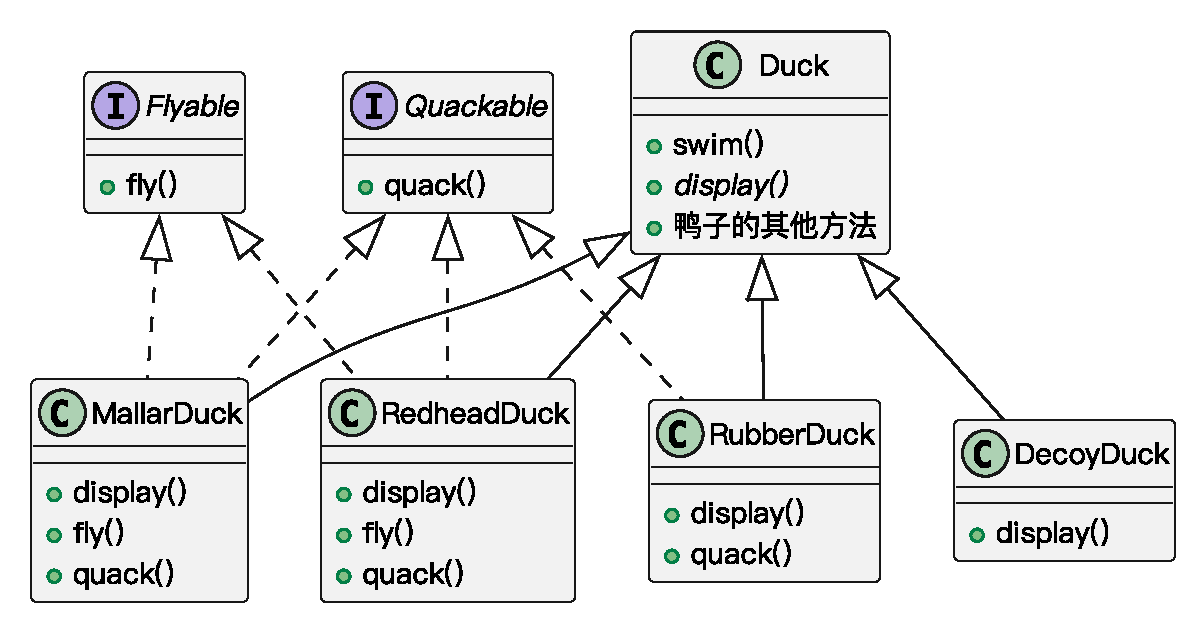
\includegraphics[width=0.75\textwidth]{images/SimUDuck3.eps}
    \vspace{-1em}
\end{figure}

\subsubsection{分开变化和不变的部分}
我们知道\;\verb|Duck|\;类内的\;\verb|fly()|\;和\;\verb|quack()|\;会随着鸭子的不同而改变。为了要把这两个行为从\;\verb|Duck|\;类中分开,我们将把它们从\;\verb|Duck|\;类中取出来,建立一组新类来代表每个行为。
\begin{figure}[H]
    \vspace{-0.5em}
	\centering
	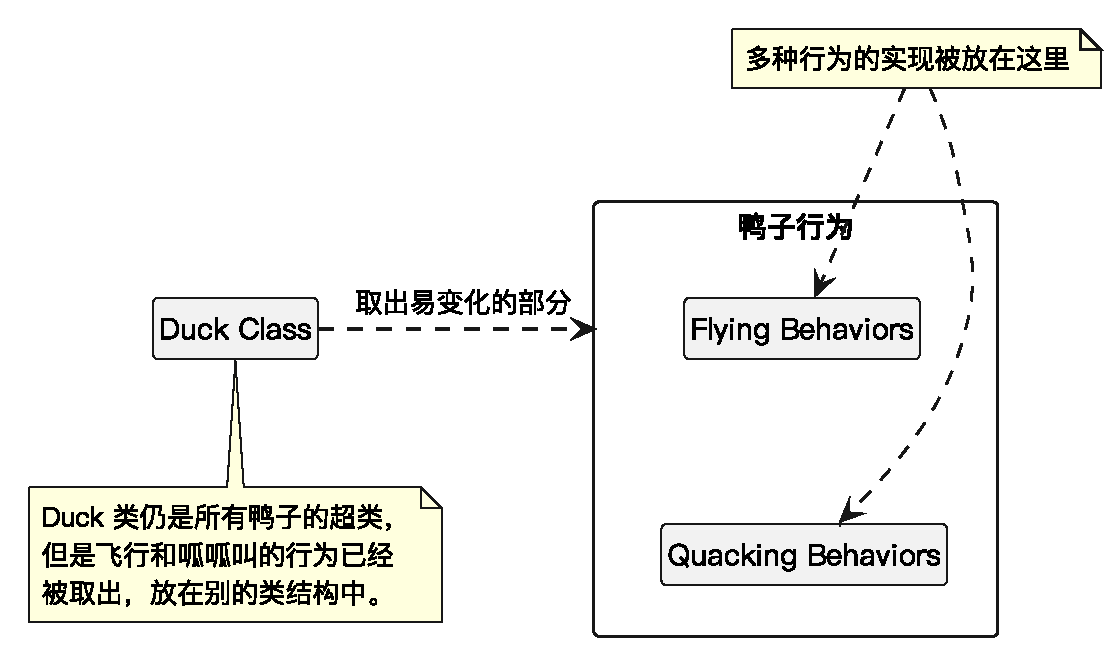
\includegraphics[width=0.65\textwidth]{images/SimUDuck4.eps}
    \vspace{-1em}
\end{figure}

\subsubsection{面向接口编程,而不是面向实现编程}
下图所示的设计,可以让飞行和呱呱叫的动作被其他的对象复用,因为这些行为已经与鸭子类无关了。而且我们可以新增一些行为,不会影响到既有的行为类,也不会影响使用到飞行行为的鸭子类。这样一来,有了继承的复用好处,却没有继承所带来的包袱。
\begin{figure}[H]
    \vspace{-0.5em}
	\centering
	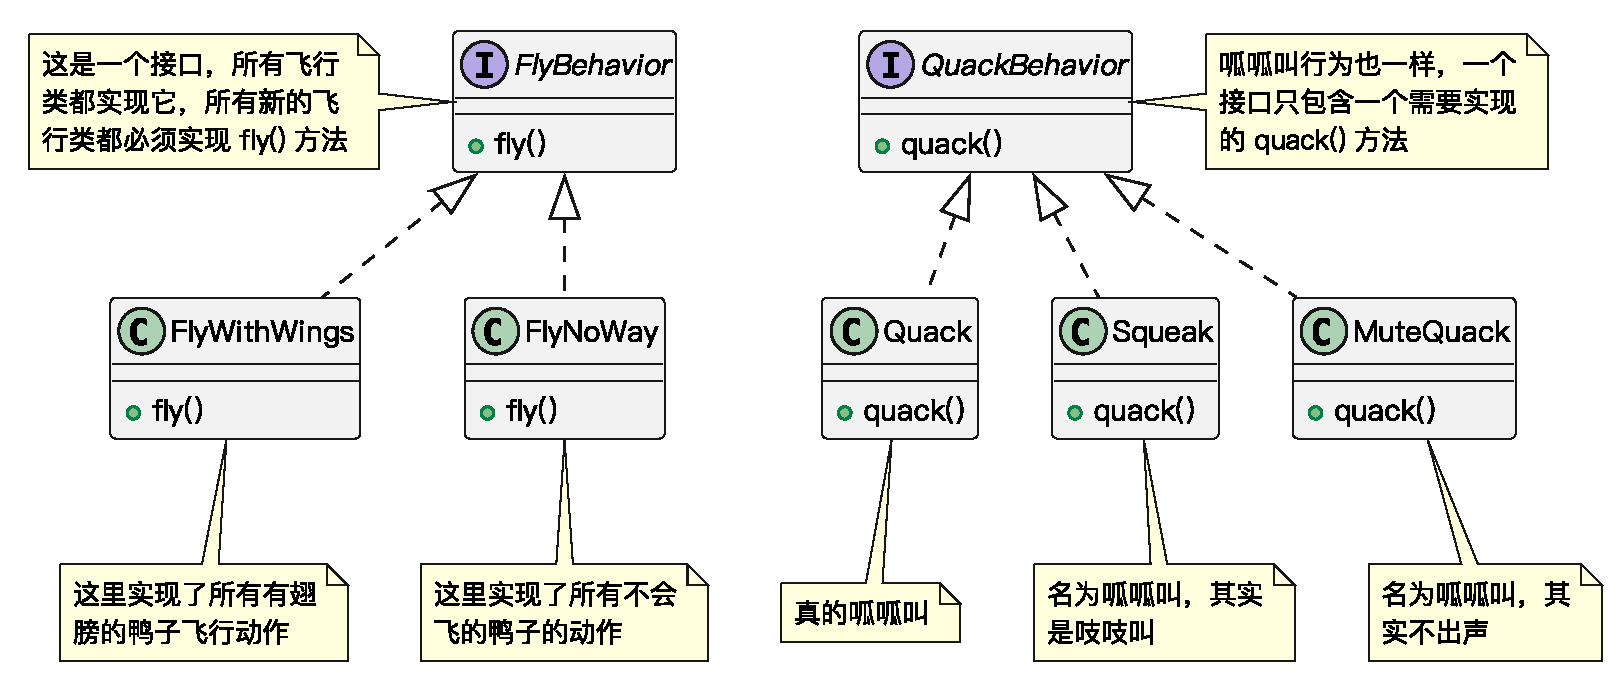
\includegraphics[width=0.9\textwidth]{images/SimUDuck5.eps}
    \vspace{-1em}
\end{figure}

\subsubsection{整合鸭子行为}
\begin{figure}[H]
    \vspace{-0.5em}
	\centering
	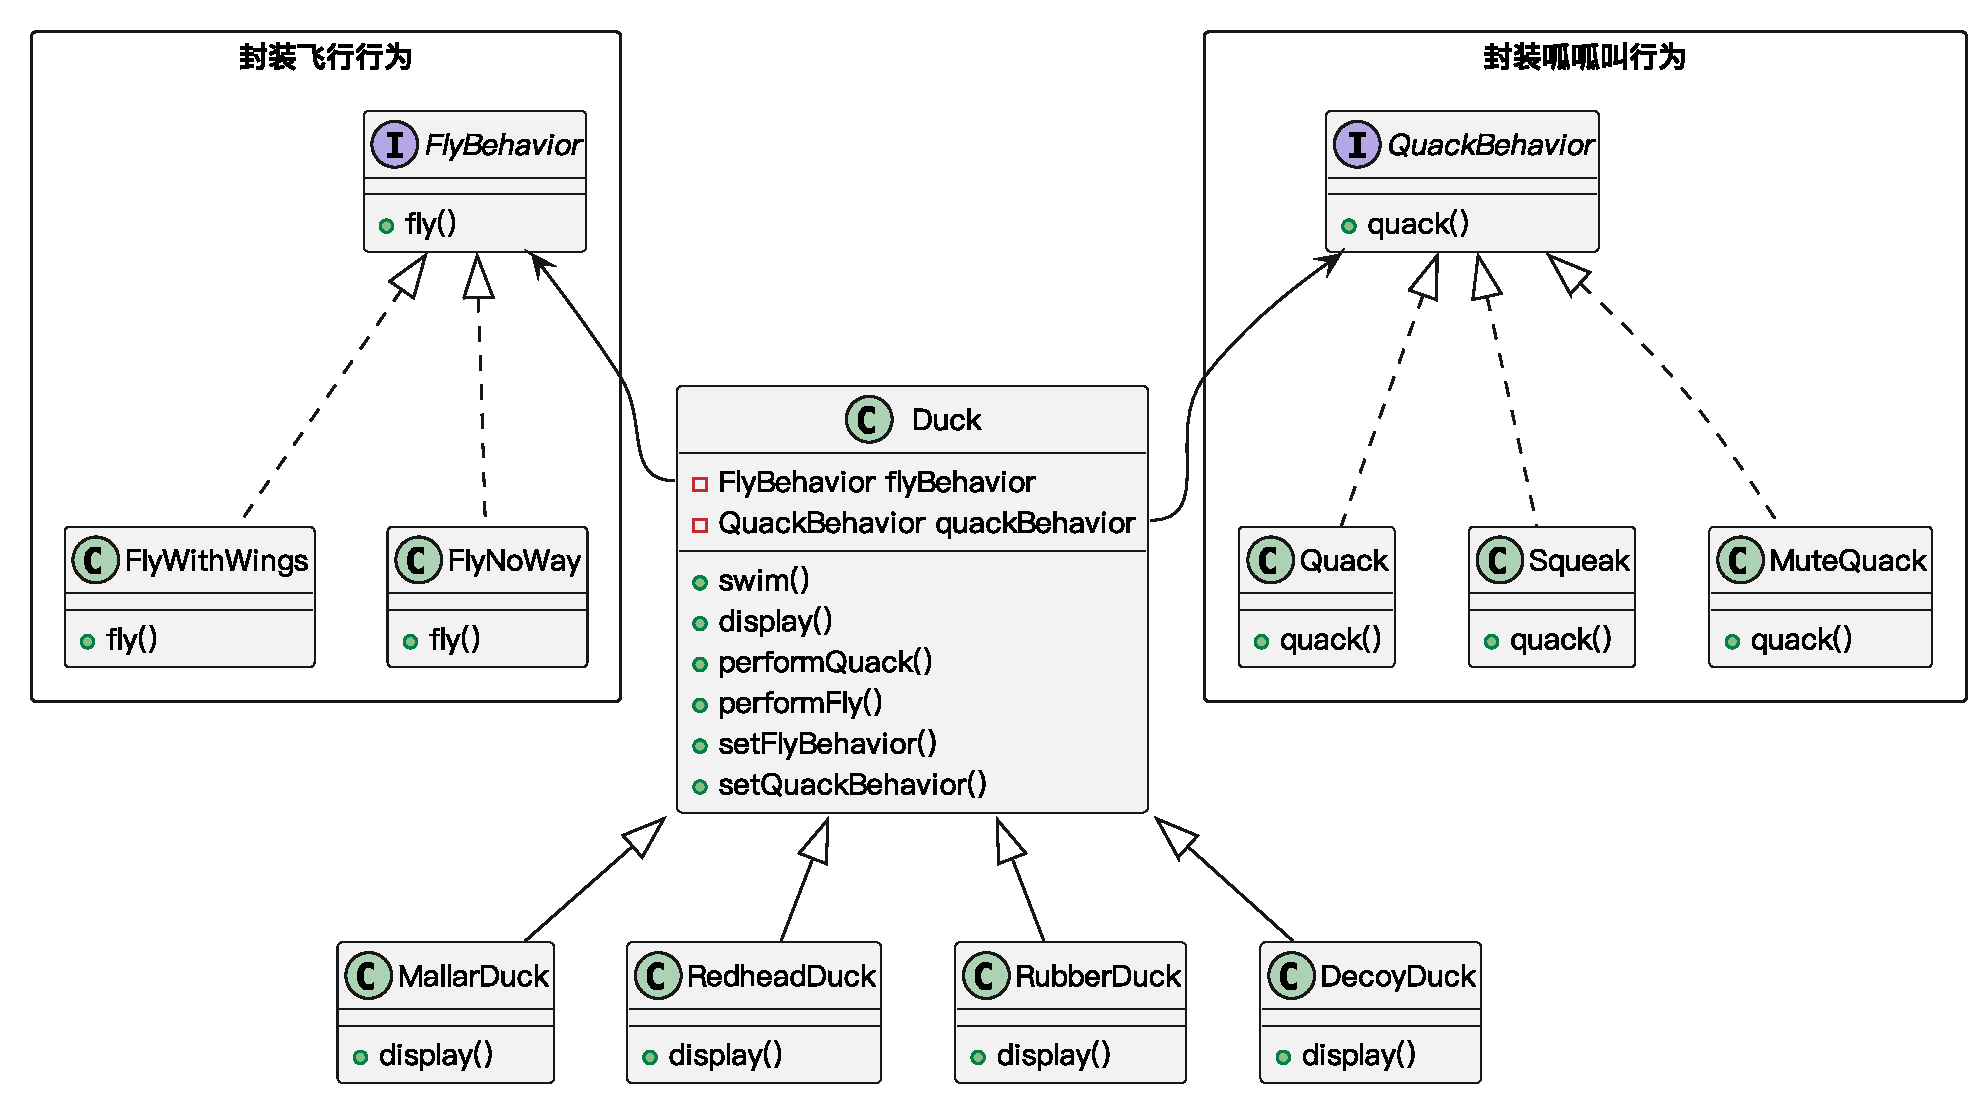
\includegraphics[width=0.95\textwidth]{images/SimUDuck6.eps}
    \vspace{-1em}
\end{figure}


\subsection{第一个设计模式:策略模式}
策略模式(Strategy Pattern)定义了一系列算法,分别封装起来,并使它们可替换。此模式让算法的变化独立于使用算法的客户。

\subsubsection{策略模式使用实例}
将文本流分成几行。由于存在许多用于将文本流分成行的算法,将所有这样的算法硬连接到类中是不可取的。
\begin{figure}[H]
    \vspace{-0.5em}
	\centering
	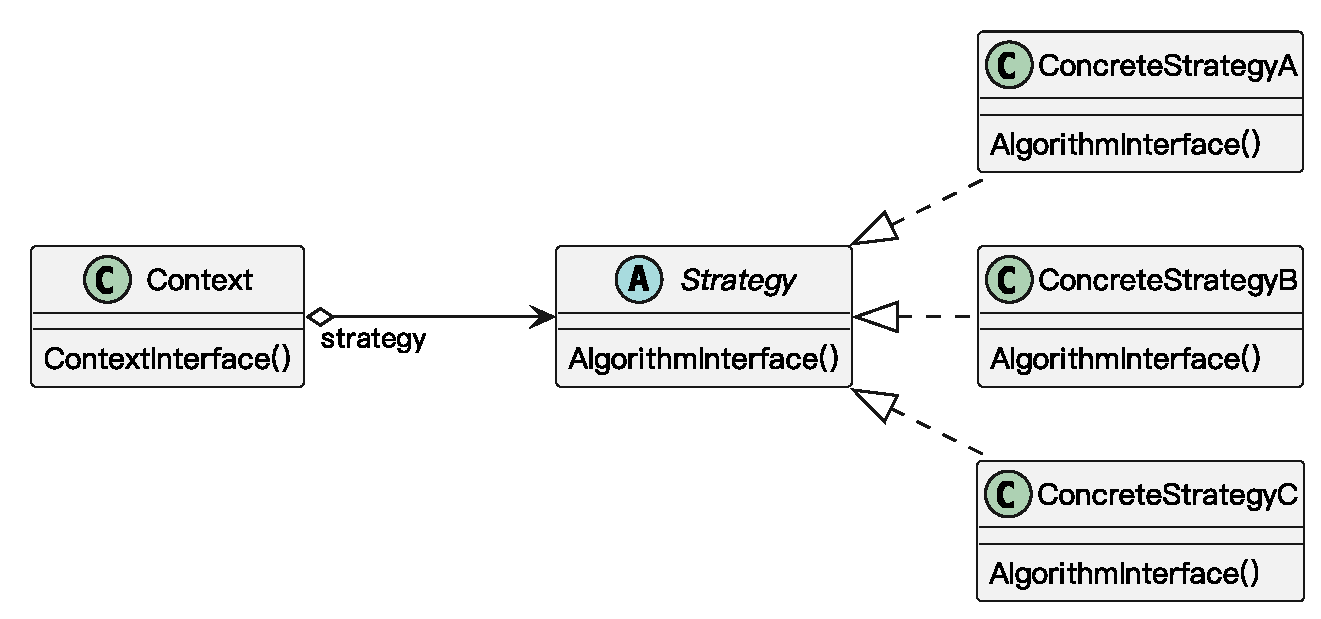
\includegraphics[width=0.58\textwidth]{images/策略模式.eps}
    \vspace{-1em}
\end{figure}


\begin{lstlisting}
public class Context{
    public void algorithm(String type){
        if(type.equals("strategyA")) {
            this.strategy = new ConcreteStrategyA();
        } else if(type.equals("strategyB")) {
            this.strategy = new ConcreteStrategyB();
        } else if(type.equals("strategyC")) {
            this.strategy = new ConcreteStrategyC();
        }
    }
}
\end{lstlisting}

\subsubsection{策略模式的使用场景}
\begin{itemize}
    \item 许多相关的类仅在\textbf{行为}上有所不同,策略提供了一种使用多种行为之一配置类的方法
    \item 需要\textbf{算法的不同变体}。例如,您定义了反映不同空间/时间权衡的算法,将这些变体实现为算法的类层次结构时,可以使用策略。
    \item 一种算法使用客户端不应该知道的数据。使用策略模式\textbf{可避免暴露复杂的、特定于算法的数据结构}。
    \item 一个类定义了许多行为,这些行为在其操作中显示为多个条件语句。此时可以代替这些条件,将相关的条件分支移到他们自己的\textbf{策略类}中。
\end{itemize}

\subsubsection{策略模式使用的结果}
\begin{itemize}
    \item 定义了相关算法家族。策略类的层次结构定义了一系列算法或行为,以供上下文重用。继承可以帮助排除算法的通用功能。
    \item 子类化的替代方法。
    \item 策略消除条件语句。
    \item 多种实现方式。策略可以提供相同行为的不同实现。客户可以选择具有不同时间和空间权衡的策略。
    \item 客户必须意识到不同的策略。这种模式有一个潜在的缺点,即\textbf{客户在选择合适的策略之前必须先了解策略的不同},不然客户可能会遇到实现问题。
    \item 策略和上下文之间的通信开销。
    \item 对象数量增加。
    \item  模式一般都会有的缺点:
    \begin{itemize}
        \item 增加设计的复杂度和增加类的个数(增加辅助类)
        \item 增加隔阂和方法调用,降低软件运行的效率,但是已经不是目前主要的问题
    \end{itemize}
    \item Java的加密方法、时间显示算法等都是通过策略模式实现的。
\end{itemize}
	\section{工厂模式}

\subsection{简单工厂模式}

\subsubsection{模式动机}
考虑一个简单的软件应用场景,一个软件系统可以提供多个外观不同的按钮(如圆形按钮、矩形 按钮、菱形按钮等),这些按钮都源自同一个基类,不过在继承基类后不同的子类修改了部分属性从而使得它们可以呈现不同的外观,如果我们希望在使用这些按钮时,不需要知道这些具体按钮类的名字,只需要知道表示该按钮类的一个参数,并提供一个调用方便的方法,把该参数传入方法即可返回一个相应的按钮对象,此时就可以使用简单工厂模式。

\subsubsection{模式定义}
简单工厂模式(Simple Factory Pattern),又称静态工厂方法(Static Factory Method)模式,它属于类创建型模式。在简单工厂模式中,可以根据参数的不同返回不同类的实例。简单工厂模式专门定义一个类来负责创建其他类的实例,被创建的实例通常都具有共同的父类。

\subsubsection{模式结构}
简单工厂模式包含如下角色:
\begin{itemize}
    \item \verb|Factory|:工厂角色
    \item \verb|Product|:抽象产品角色
    \item \verb|ConcreteProduct|:具体产品角色
\end{itemize}

\begin{figure}[H]
    \vspace{-0.5em}
	\centering
	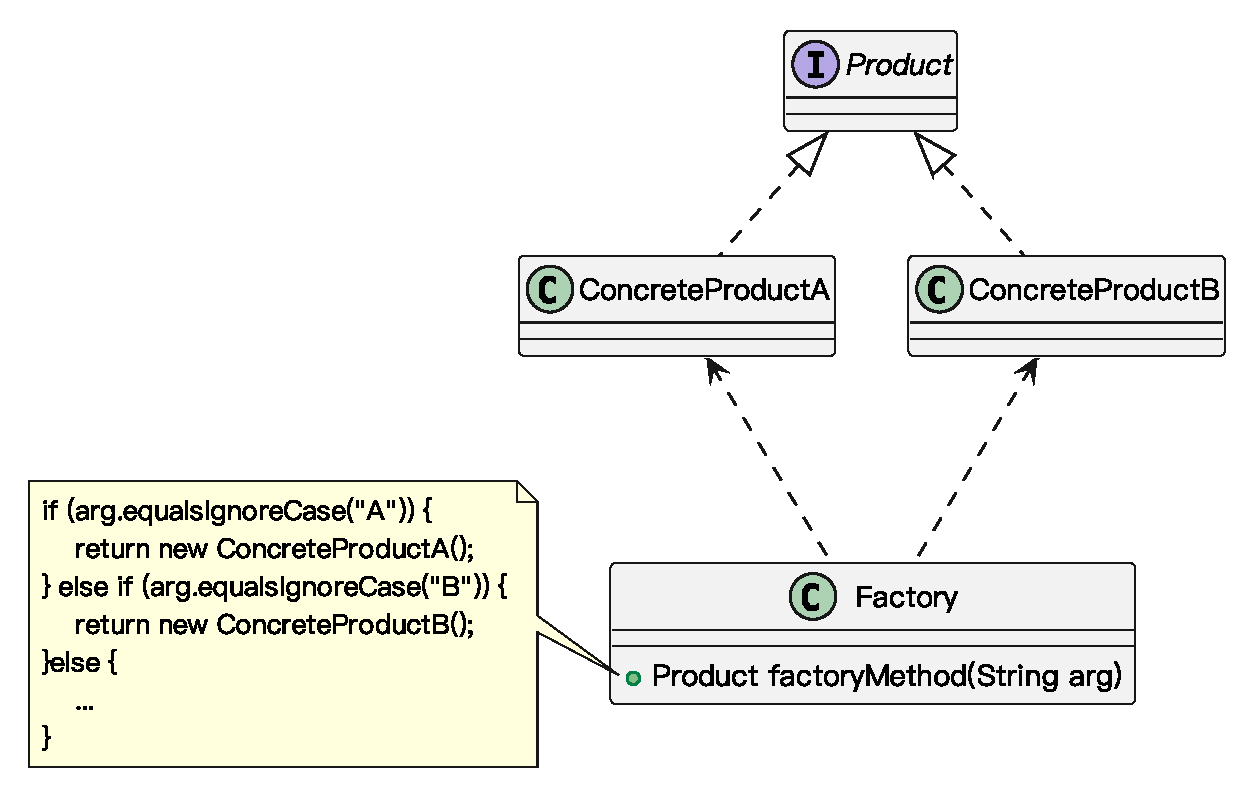
\includegraphics[width=0.7\textwidth]{images/简单工厂模式.eps}
    \vspace{-1em}
\end{figure}

\subsubsection{模式分析}
\begin{itemize}
    \item \textbf{将对象的创建和对象本身业务处理分离可以降低系统的耦合度},使得两者修改起来都相对容易。
    \item 在调用工厂类的工厂方法时,由于工厂方法是\textbf{静态方法},使用起来很方便,可通过类名直接调用,而且只需要传入一个简单的参数即可,在实际开发中,还可以在调用时将所传入的参数保存在XML等格式的\textbf{配置文件中},修改参数时无须修改任何Java源代码。
    \item 简单工厂模式最大的问题在于\textbf{工厂类的职责相对过重},增加新的产品需要修改工厂类的判断逻辑,这一点与开闭原则是相违背的。
    \item 简单工厂模式的要点在于:\textbf{当你需要什么,只需要传入一个正确的参数,就可以获取你所需要的对象,而无须知道其创建细节}。
\end{itemize}
\begin{figure}[H]
    \vspace{-0.5em}
	\centering
	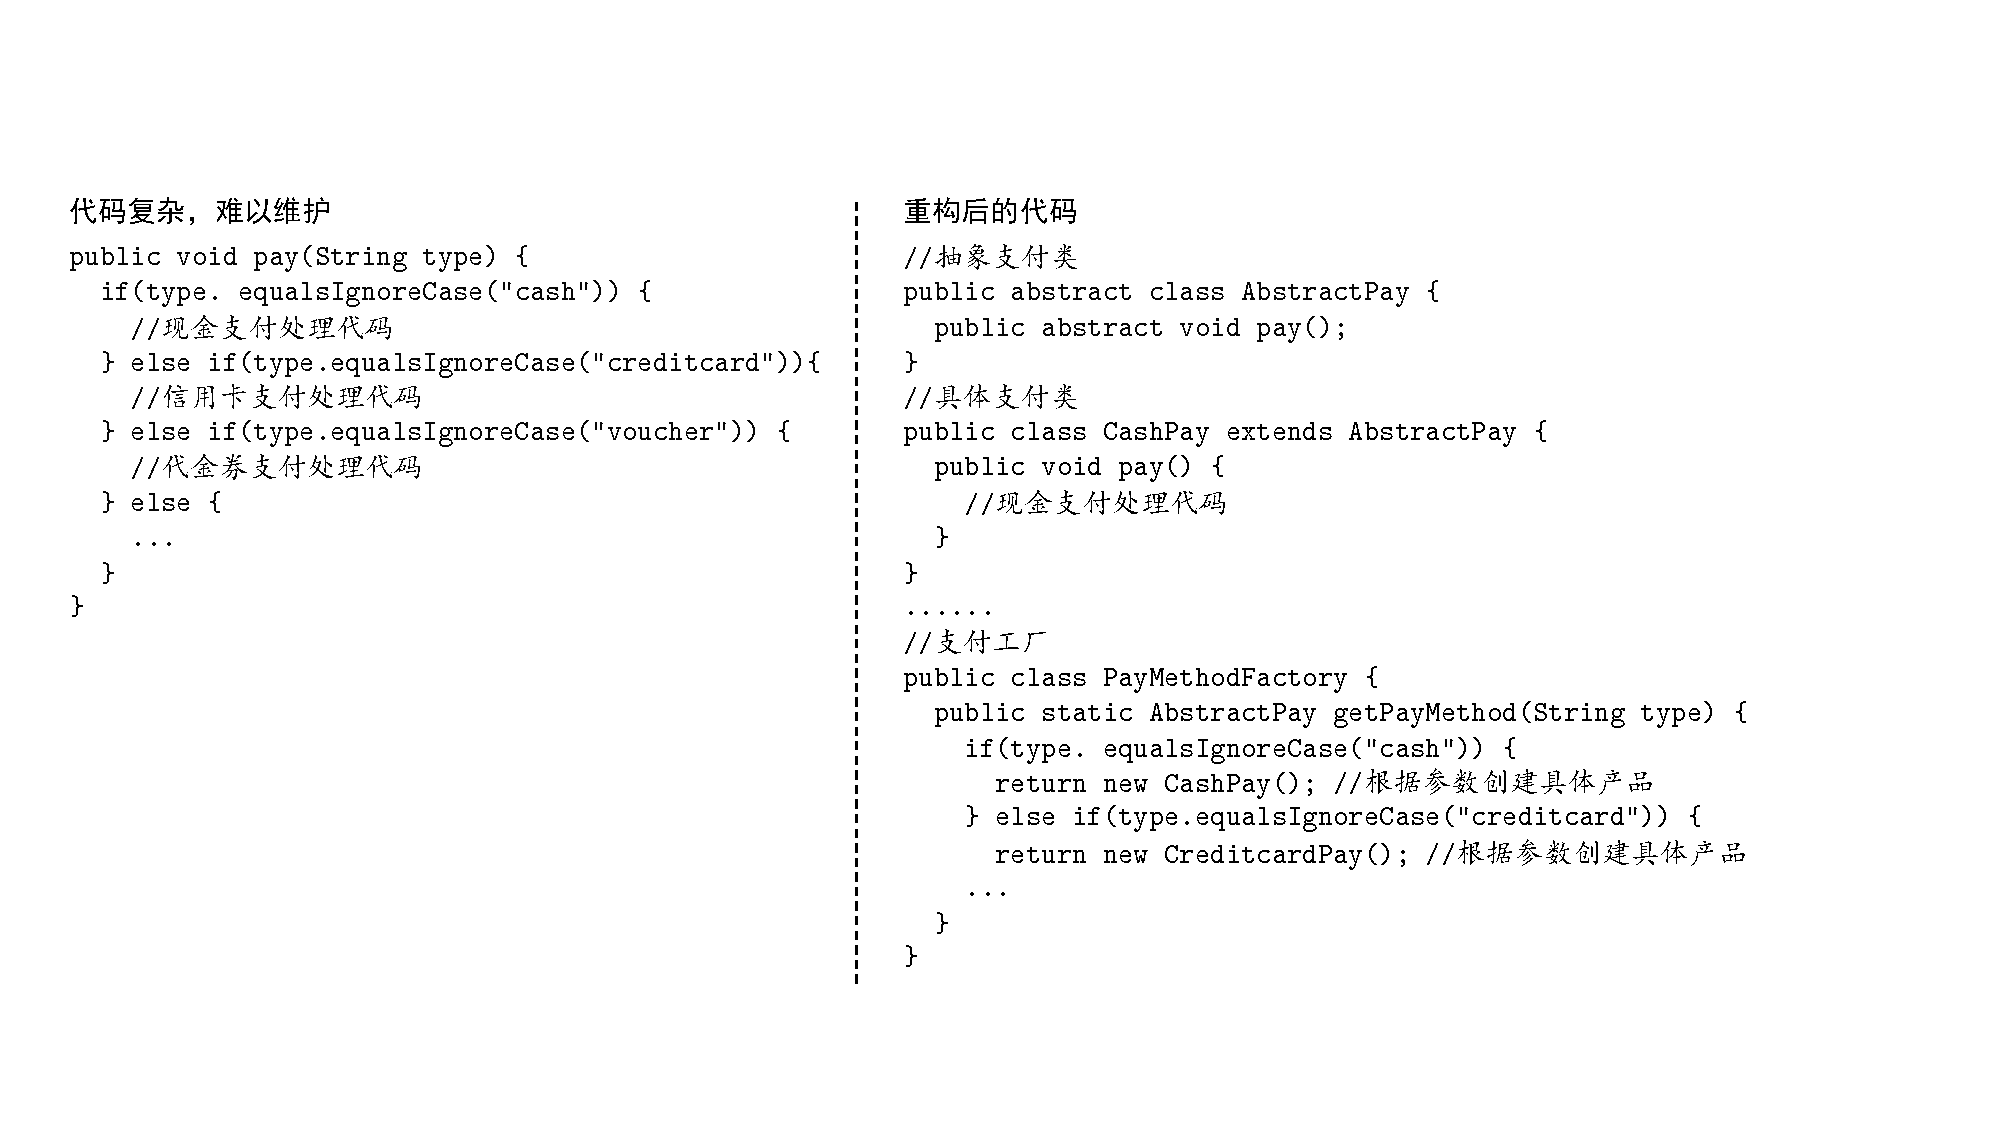
\includegraphics[width=\textwidth]{images/简单工厂模式分析.pdf}
    \vspace{-1.5em}
\end{figure}

\subsubsection{模式实例}
权限管理:在某OA系统中,系统根据对比用户在登录时输入的账号和密码以及在数据库中存储的账号和密码是否一致来进行身份验证,如果验证通过,则取出存储在数据库中的用户权限等级(以整数形式存储),根据不同的权限等级创建不同等级的用户对象,不同等级的用户对象拥有不同的操作权限。现使用简单工厂模式来设计该权限管理模块。
\begin{figure}[H]
    \vspace{-0.5em}
	\centering
	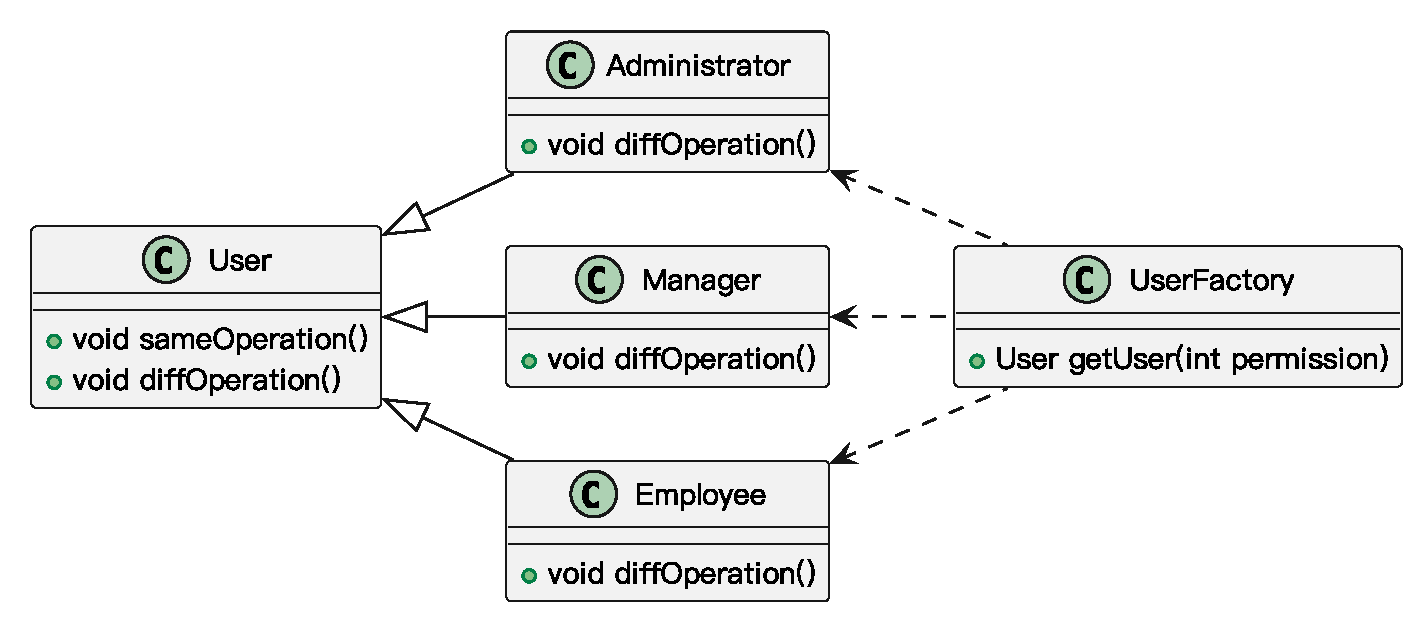
\includegraphics[width=0.85\textwidth]{images/简单工厂模式实例.eps}
    \vspace{-1em}
\end{figure}

\subsubsection{模式优缺点}
简单工厂模式的优点
\begin{itemize}
    \item 工厂类含有必要的判断逻辑,可以决定在什么时候创建哪一个产品类的实例,客户端可以免除直接创建产品对象的责任,而仅仅“消费”产品;简单工厂模式通过这种做法\textbf{实现了对责任的分割,它提供了专门的工厂类用于创建对象}。
    \item \textbf{客户端无须知道所创建的具体产品类的类名,只需要知道具体产品类所对应的参数即可},对于一些复杂的类名,通过简单工厂模式可以减少使用者的记忆量。
    \item \textbf{通过引入配置文件,可以在不修改任何客户端代码的情况下更换和增加新的具体产品类},在一定程度上提高了系统的灵活性。
\end{itemize}
简单工厂模式的缺点
\begin{itemize}
    \item 由于\textbf{工厂类集中了所有产品创建逻辑},一旦不能正常工作,整个系统都要受到影响。
    \item 使用简单工厂模式将会\textbf{增加系统中类的个数},在一定程序上增加了系统的复杂度和理解难度。
    \item \textbf{系统扩展困难,一旦添加新产品就不得不修改工厂逻辑},在产品类型较多时,有可能造成工厂逻辑过于复杂,不利于系统的扩展和维护。只是把分散在系统各个地方的变化汇总到了一起。
    \item 简单工厂模式由于使用了静态工厂方法,造成\textbf{工厂角色无法形成基于继承的等级结构}。
\end{itemize}

\subsubsection{模式适用环境}
在以下情况下可以使用简单工厂模式:
\begin{itemize}
    \item \textbf{工厂类负责创建的对象比较少}:由于创建的对象较少,不会造成工厂方法中的业务逻辑太过复杂(如果扩展使比较少的)
    \item \textbf{客户端只知道传入工厂类的参数,对于如何创建对象不关心}:客户端既不需要关心创建细节,甚至连类名都不需要记住,只需要知道类型所对应的参数(比如只知道名称参数)
\end{itemize}

\subsubsection{模式应用}
在JDK类库中广泛使用了简单工厂模式,如工具类\;\verb|java.text.DateFormat|,它用于格式化一个本地日期或者时间。
\begin{lstlisting}
public final static DateFormat getDateInstance();
public final static DateFormat getDateInstance(int style);
public final static DateFormat getDateInstance(int style, Locale locale);
\end{lstlisting}

Java加密技术
\begin{lstlisting}
//获取不同加密算法的密钥生成器
KeyGenerator keyGen = KeyGenerator.getInstance("DESede");
//创建密码器
Cipher cp = Cipher.getInstance("DESede");
\end{lstlisting}

\subsubsection{模式扩展}
简单工厂模式的简化:在有些情况下工厂类可以由抽象产品角色扮演,一个抽象产品类同时也是子类的工厂,也就是说把静态工厂方法写到抽象产品类中。
\begin{figure}[H]
    \vspace{-0.5em}
	\centering
	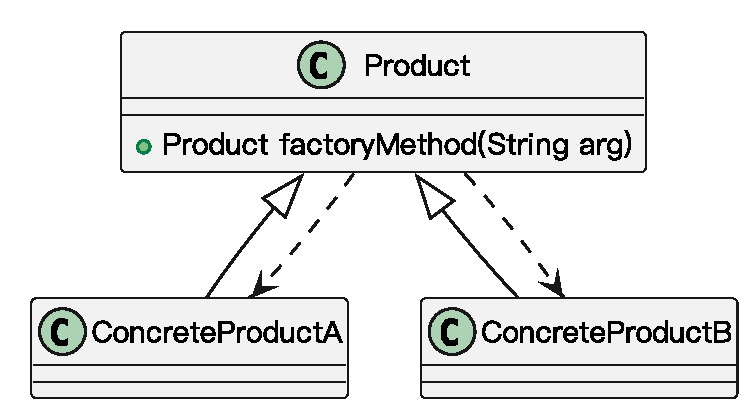
\includegraphics[width=0.5\textwidth]{images/简单工厂模式的简化.eps}
    \vspace{-1em}
\end{figure}

\subsection{工厂方法模式}

\subsubsection{工厂模式的引入}
简单工厂模式的不足:在简单工厂模式中,只提供了一个工厂类,该工厂类处于对产品类进行实例化的中心位置,它知道每一个产品对象的创建细节,并决定何时实例化哪一个产品类。\textbf{简单工厂模式最大的缺点是当有新产品要加入到系统中时,必须修改工厂类,加入必要的处理逻辑,这违背了“开闭原则”。}在简单工厂模式中,所有的产品都是由同一个工厂创建,工厂类职责较重,业务逻辑较为复杂,具体产品与工厂类之间的耦合度高,严重影响了系统的灵活性和扩展性,而工厂方法模式则可以很好地解决这一问题。

\subsubsection{模式动机}
考虑这样一个系统,按钮工厂类可以返回一个具体的按钮实例,如圆形按钮、矩形按钮、菱形按钮等。在这个系统中,如果需要增加一种新类型的按钮,如椭圆形按钮,那么\textbf{除了增加一个新的具体产品类之外,还需要修改工厂类的代码,这就使得整个设计在一定程度上违反了“开闭原则”。}

现在对该系统进行修改,不再设计一个按钮工厂类来统一负责所有产品的创建,而是\textbf{将具体按钮的创建过程交给专门的工厂子类去完成},我们\textbf{先定义一个抽象的按钮工厂类,再定义具体的工厂类来生成圆形按钮、矩形按钮、菱形按钮等},它们实现在抽象按钮工厂类中定义的方法。这种抽象化的结果使这种结构\textbf{可以在不修改具体工厂类的情况下引进新的产品},如果出现新的按钮类型,只需要为这种新类型的按钮创建一个具体的工厂类就可以获得该新按钮的实例,这一特点无疑使得工厂方法模式具有超越简单工厂模式的优越性,\textbf{更加符合“开闭原则” }。
\begin{figure}[H]
    \vspace{-0.5em}
	\centering
	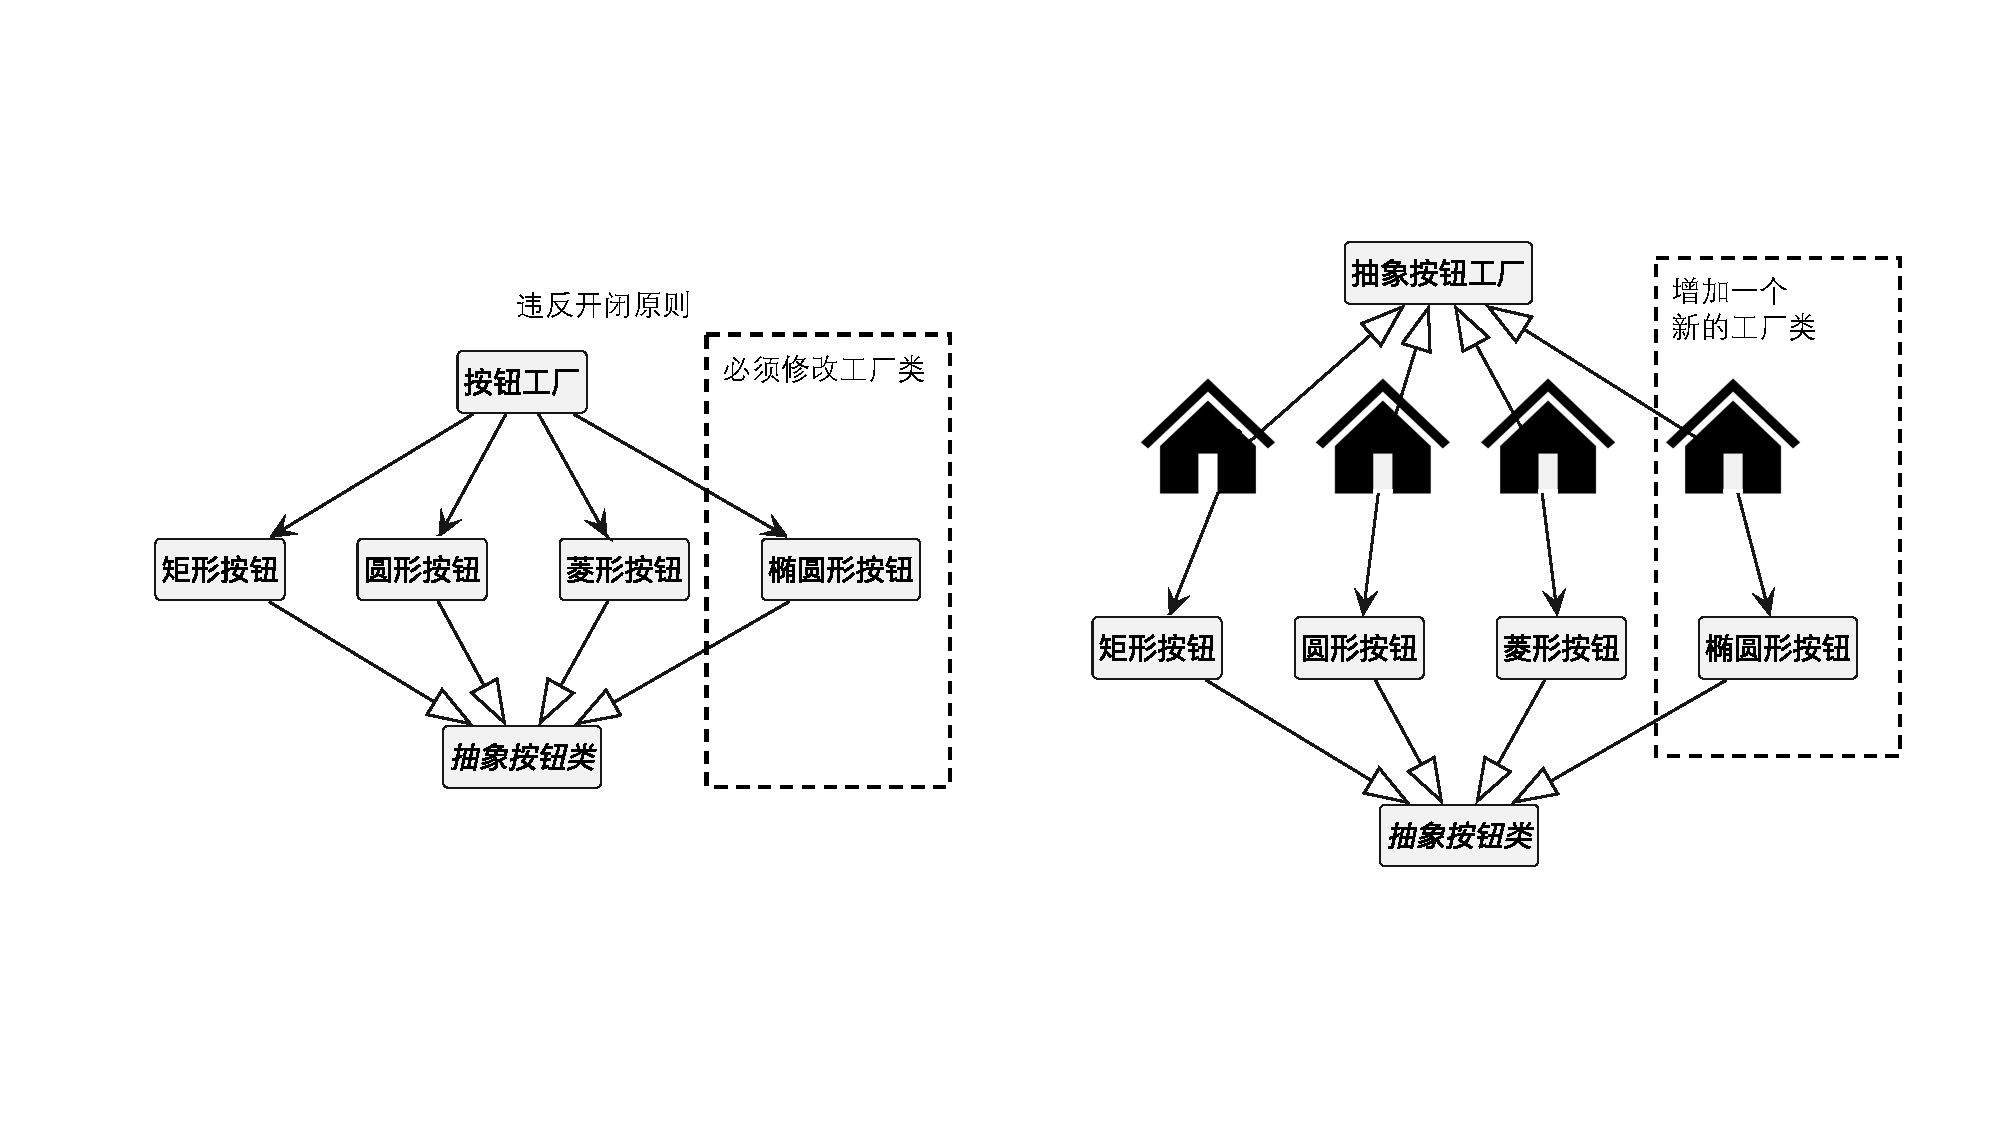
\includegraphics[width=0.75\textwidth]{images/工厂模式动机.pdf}
    \vspace{-1em}
\end{figure}

\subsubsection{模式定义}
工厂方法模式(Factory Method Pattern)又称为工厂模式,也叫虚拟构造器(Virtual Constructor)模式或者多态工厂(Polymorphic Factory)模式,它属于类创建型模式。在工厂方法模式中,工厂父类负责定义创建产品对象的公共接口,而工厂子类则负责生成具体的产品对象,这样做的目的是将产品类的实例化操作延迟到工厂子类中完成,即通过工厂子类来确定究竟应该实例化哪一个具体产品类。

\subsubsection{模式结构}
\begin{figure}[H]
    \vspace{-0.5em}
	\centering
	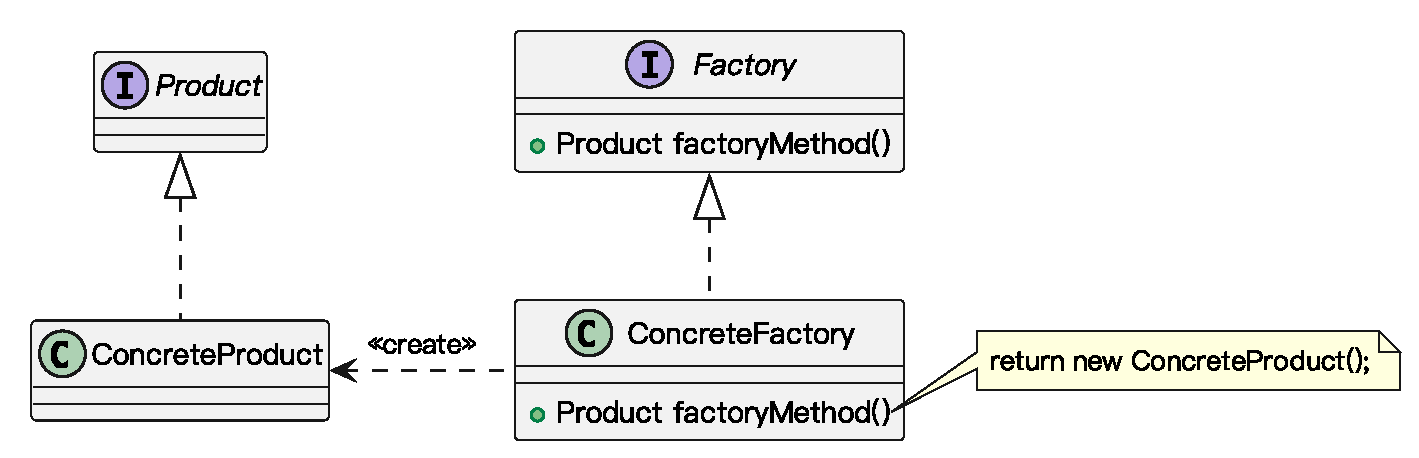
\includegraphics[width=0.75\textwidth]{images/工厂模式结构.eps}
    \vspace{-1em}
\end{figure}

\subsubsection{模式分析}
\begin{itemize}
    \item 工厂方法模式是简单工厂模式的进一步抽象和推广。由于使用了面向对象的多态性,工厂方法模式保持了简单工厂模式的优点,而且克服了它的缺点。\textbf{在工厂方法模式中,核心的工厂类不再负责所有产品的创建,而是将具体创建工作交给子类去做。}这个核心类仅仅负责给出具体工厂必须实现的接口,而不负责哪一个产品类被实例化这种细节,这使得\textbf{工厂方法模式可以允许系统在不修改工厂角色的情况下引进新产品}。
    \item 当系统扩展需要添加新的产品对象时,仅仅需要添加一个具体产品对象以及一个具体工厂对象,原有工厂对象不需要进行任何修改,也不需要修改客户端,\textbf{很好地符合了“开闭原则”}。而简单工厂模式在添加新产品对象后不得不修改工厂方法,扩展性不好。\textbf{工厂方法模式退化后可以演变成简单工厂模式}。
\end{itemize}

为了提高系统的可扩展性和灵活性,\textbf{在定义工厂和产品时都必须使用抽象层},如果需要更换产品类,只需要更换对应的工厂即可,其他代码不需要进行任何修改。
\begin{lstlisting}
//抽象工厂类代码
public abstract class PayMethodFactory{
    public abstract AbstractPay getPayMethod();
}
//具体工厂类代码
public class CashPayFactory extends PayMethodFactory{
    public AbstractPay getPayMethod(){
        return new CashPay();
    }
}
//客户类代码片段
PayMethodFactory factory;
AbstractPay payMethod;
factory = new CashPayFactory();
payMethod =factory.getPayMethod();
payMethod.pay();
\end{lstlisting}

在实际的应用开发中,一般将具体工厂类的实例化过程进行改进,不直接使用\;\verb|new|\;关键字来创建对象,而是将具体类的类名写入\textbf{配置文件}中,再通过Java的\textbf{反射机制},读取XML格式的配置文件,根据存储在XML文件中的类名字符串生成对象。
\begin{figure}[H]
    \vspace{-0.5em}
	\centering
	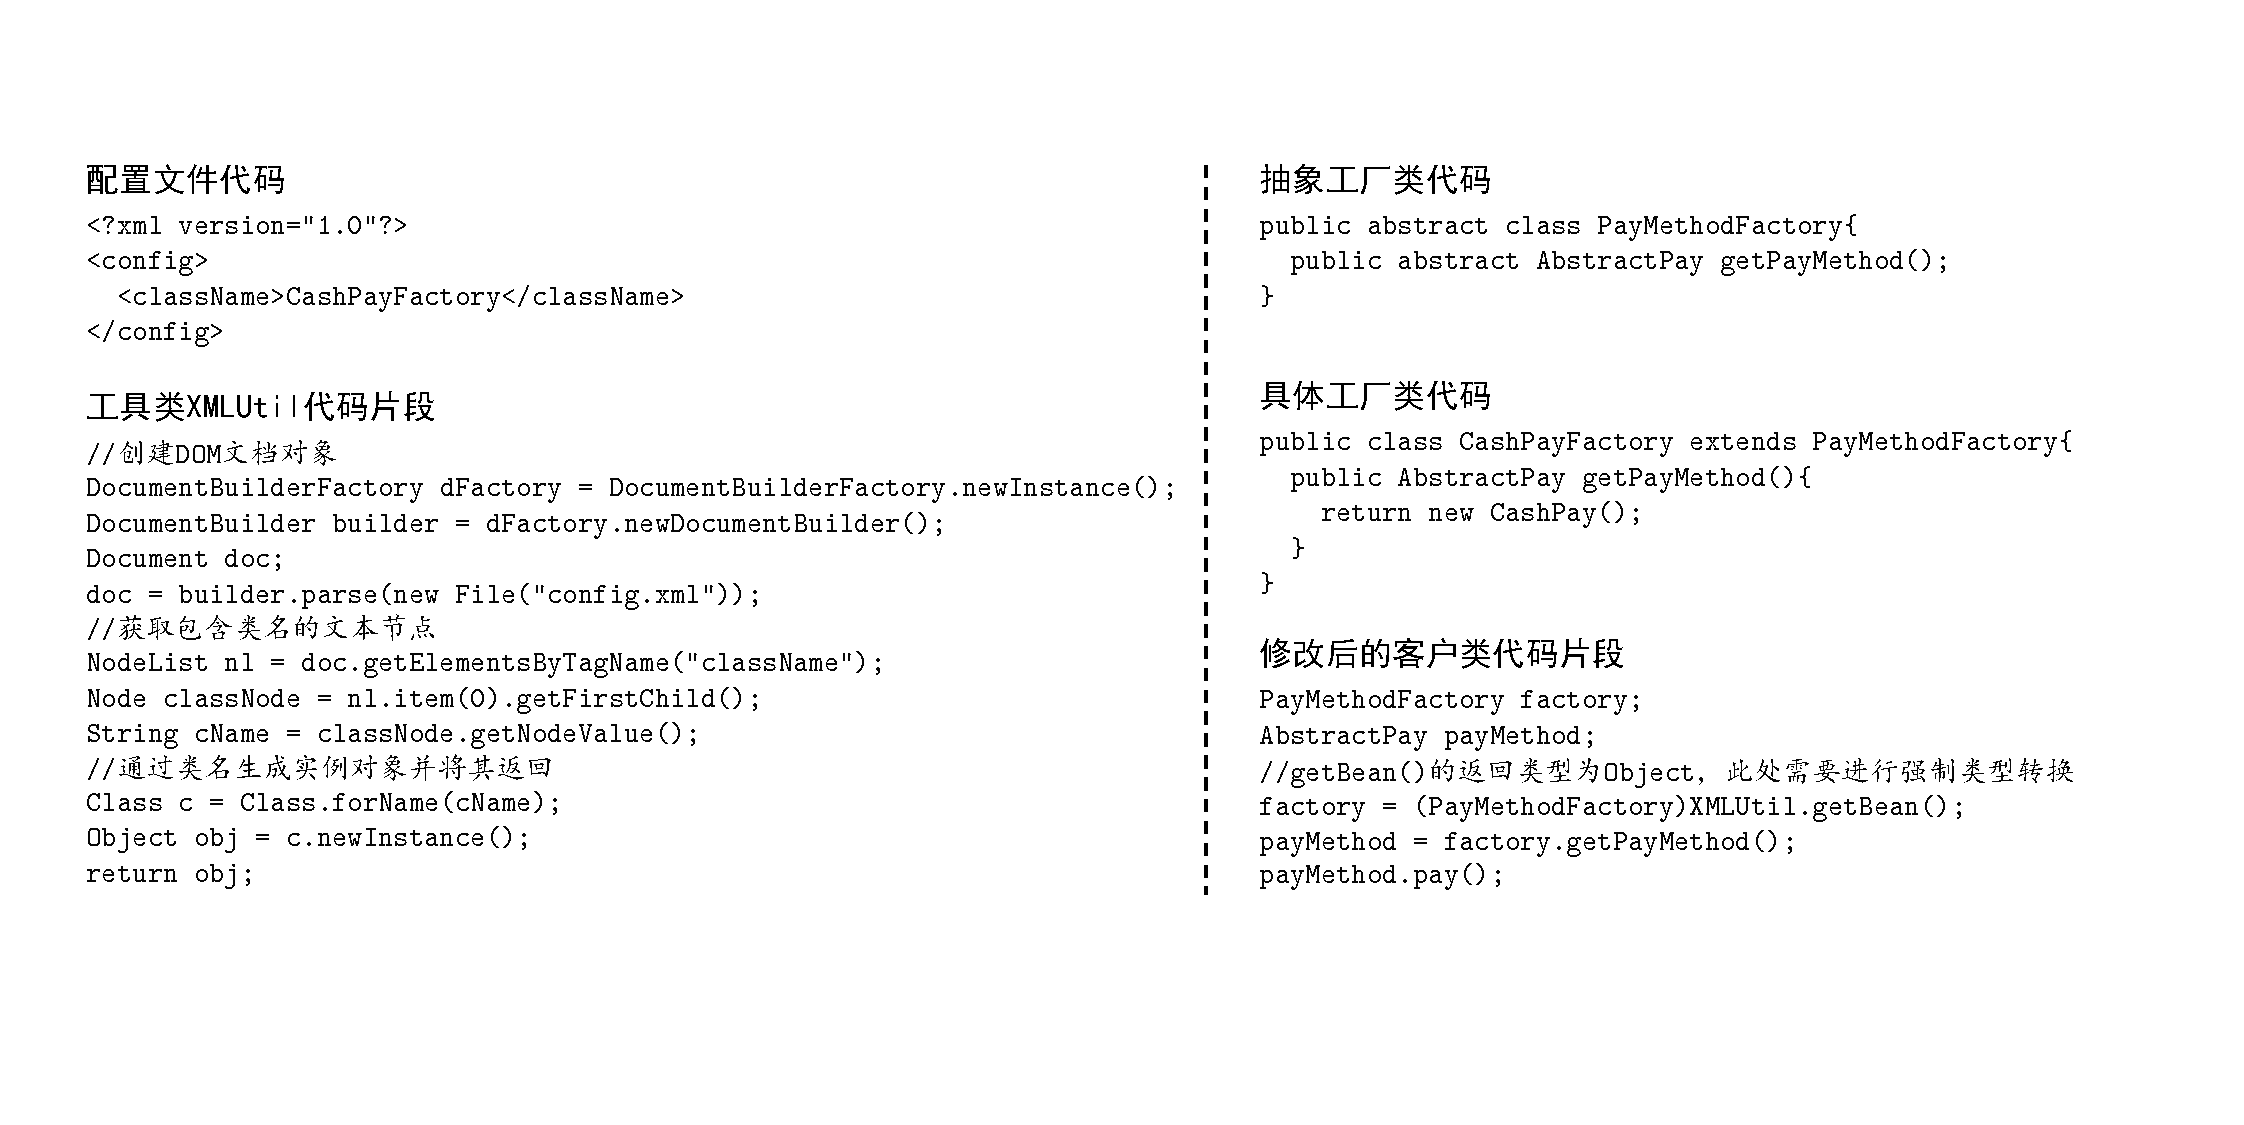
\includegraphics[width=\textwidth]{images/工厂模式分析.pdf}
    \vspace{-2em}
\end{figure}

\vspace{-0.5em}
\begin{shaded}
Java反射(Java Reflection):是指在程序运行时获取已知名称的类或已有对象的相关信息的一种机制,包括类的方法、属性、超类等信息,还包括实例的创建和实例类型的判断等。可通过\;\verb|Class|\;类的\;\verb|forName()|\;方法返回与带有给定字符串名的类或接口相关联的\;\verb|Class|\;对象,再通过\;\verb|newInstance()|\;方法创建此对象所表示的类的一个新实例,即通过一个类名字符串得到类的实例。
\begin{lstlisting}
//创建一个字符串类型的对象
Class c = Class.forName("String");
Object obj = c.newInstance();
return obj;
\end{lstlisting}
\end{shaded}
\vspace{-1em}

\subsubsection{模式实例}
日志记录器:某系统日志记录器要求支持多种日志记录方式,如文件记录、数据库记录等,且用户可以根据要求动态选择日志记录方式,现使用工厂方法模式设计该系统。
\begin{figure}[H]
    \vspace{-0.5em}
	\centering
	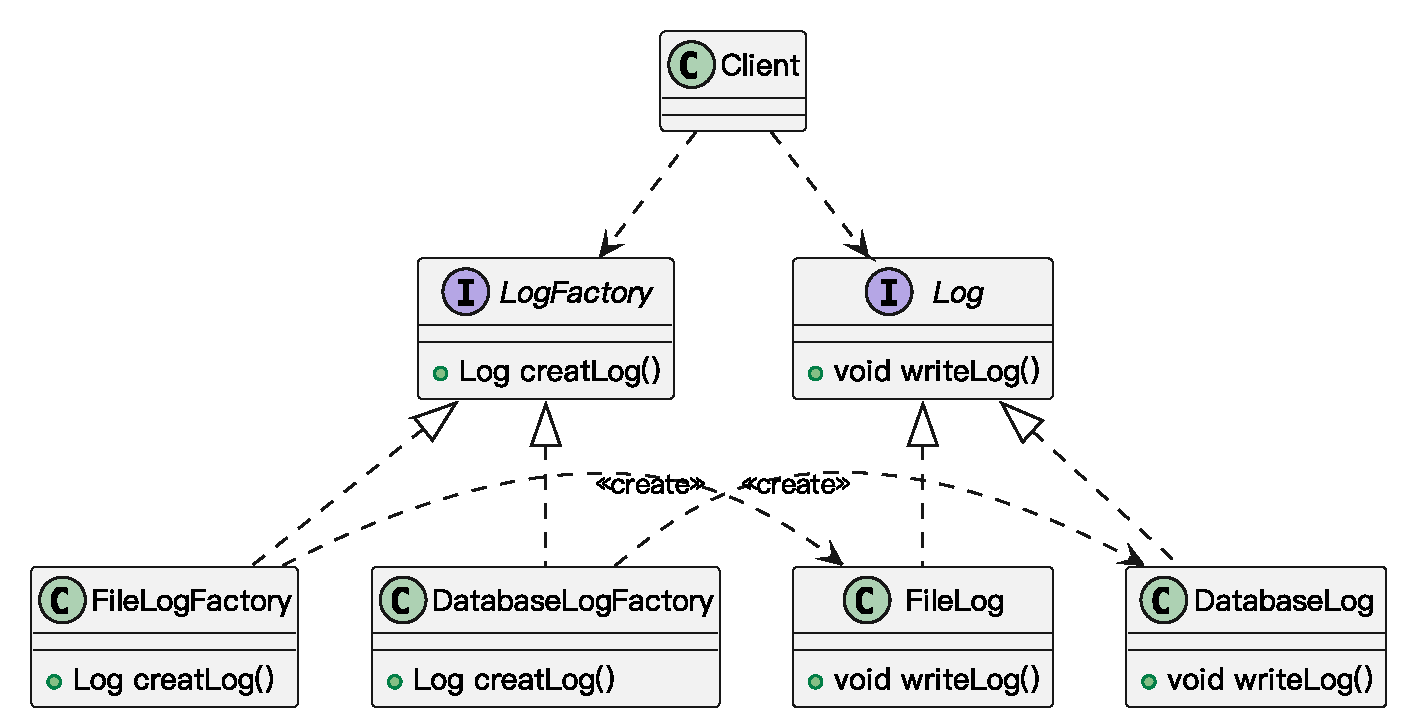
\includegraphics[width=0.75\textwidth]{images/工厂模式实例.eps}
    \vspace{-1em}
\end{figure}

\subsubsection{模式优缺点}
工厂方法模式的优点
\begin{itemize}
    \item 在工厂方法模式中,工厂方法用来创建客户所需要的产品,同时还向客户隐藏了哪种具体产品类将被实例化这一细节,\textbf{用户只需要关心所需产品对应的工厂,无须关心创建细节,甚至无须知道具体产品类的类名}。
    \item 基于工厂角色和产品角色的多态性设计是工厂方法模式的关键。它能够使\textbf{工厂可以自主确定创建何种产品对象,而如何创建这个对象的细节则完全封装在具体工厂内部}。工厂方法模式之所以又被称为多态工厂模式,是因为所有的具体工厂类都具有同一抽象父类。
    \item 使用工厂方法模式的另一个优点是\textbf{在系统中加入新产品时,无须修改抽象工厂和抽象产品提供的接口,无须修改客户端,也无须修改其他的具体工厂和具体产品,而只要添加一个具体工厂和具体产品就可以了}。这样,系统的可扩展性也就变得非常好,完全符合“开闭原则”。
\end{itemize}

工厂方法模式的缺点
\begin{itemize}
    \item 在添加新产品时,\textbf{需要编写新的具体产品类,而且还要提供与之对应的具体工厂类,系统中类的个数将成对增加,在一定程度上增加了系统的复杂度},有更多的类需要编译和运行,会给系统带来一些额外的开销。
    \item 由于考虑到系统的可扩展性,需要引入抽象层,在客户端代码中均使用抽象层进行定义,\textbf{增加了系统的抽象性和理解难度},且在实现时可能需要用到DOM、反射等技术,增加了系统的实现难度。
\end{itemize}

\subsubsection{模式适用环境}
在以下情况下可以使用工厂方法模式:
\begin{itemize}
    \item \textbf{一个类不知道它所需要的对象的类}:在工厂方法模式中,客户端不需要知道具体产品类的类名,只需要知道所对应的工厂即可,具体的产品对象由具体工厂类创建;客户端需要知道创建具体产品的工厂类。
    \item \textbf{一个类通过其子类来指定创建哪个对象}:在工厂方法模式中,对于抽象工厂类只需要提供一个创建产品的接口,而由其子类来确定具体要创建的对象,利用面向对象的多态性和里氏代换原则,在程序运行时,子类对象将覆盖父类对象,从而使得系统更容易扩展。
    \item \textbf{将创建对象的任务委托给多个工厂子类中的某一个,客户端在使用时可以无须关心是哪一个工厂子类创建产品子类,需要时再动态指定},可将具体工厂类的类名存储在配置文件或数据库中。
\end{itemize}


\subsection{抽象工厂模式}

\subsubsection{模式引入}
在工厂方法模式中具体工厂负责生产具体的产品,每一个具体工厂对应一种具体产品,工厂方法也具有唯一性,一般情况下,一个具体工厂中只有一个工厂方法或者一组重载的工厂方法。但是有时候我们需要\textbf{一个工厂可以提供多个产品对象,而不是单一的产品对象}。

\subsubsection{模式动机}
为了更清晰地理解工厂方法模式,需要先引入两个概念:
\begin{itemize}
    \item \textbf{产品等级结构}:产品等级结构即\textbf{产品的继承结构},如一个抽象类是电视机,其子类有海尔电视机、海信电视机、TCL电视机,则抽象电视机与具体品牌的电视机之间构成了一个产品等级结构,抽象电视机是父类,而具体品牌的电视机是其子类。
    \item \textbf{产品族}:在抽象工厂模式中,产品族是指\textbf{由同一个工厂生产的,位于不同产品等级结构中的一组产品},如海尔电器工厂生产的海尔电视机、海尔电冰箱,海尔电视机位于电视机产品等级结构中,海尔电冰箱位于电冰箱产品等级结构中。
\end{itemize}

当系统所提供的工厂所需生产的具体产品并不是一个简单的对象,而是\textbf{多个位于不同产品等级结构中属于不同类型的具体产品时}需要使用抽象工厂模式。

抽象工厂模式是所有形式的工厂模式中\textbf{最为抽象和最具一般性的一种形态}。

抽象工厂模式与工厂方法模式最大的区别在于,\textbf{工厂方法模式针对的是一个产品等级结构,而抽象工厂模式则需要面对多个产品等级结构},一个工厂等级结构可以负责多个不同产品等级结构中的产品对象的创建。当一个工厂等级结构可以创建出分属于不同产品等级结构的一个产品族中的所有对象时,抽象工厂模式比工厂方法模式更为简单、有效率。

\subsubsection{模式定义}
抽象工厂模式(Abstract Factory Pattern):\textbf{提供一个创建一系列相关或相互依赖对象的接口,而无须指定它们具体的类}。抽象工厂模式又称为Kit模式,属于对象创建型模式。

\subsubsection{模式结构}
抽象工厂模式包含如下角色:
\vspace{-0.8em}
\begin{multicols}{2}
    \begin{itemize}
        \item AbstractFactory:抽象工厂
        \item ConcreteFactory:具体工厂
        \item AbstractProduct:抽象产品
        \item Product:具体产品
    \end{itemize}
\end{multicols}
\vspace{-1em}

\begin{figure}[H]
    \vspace{-0.5em}
	\centering
	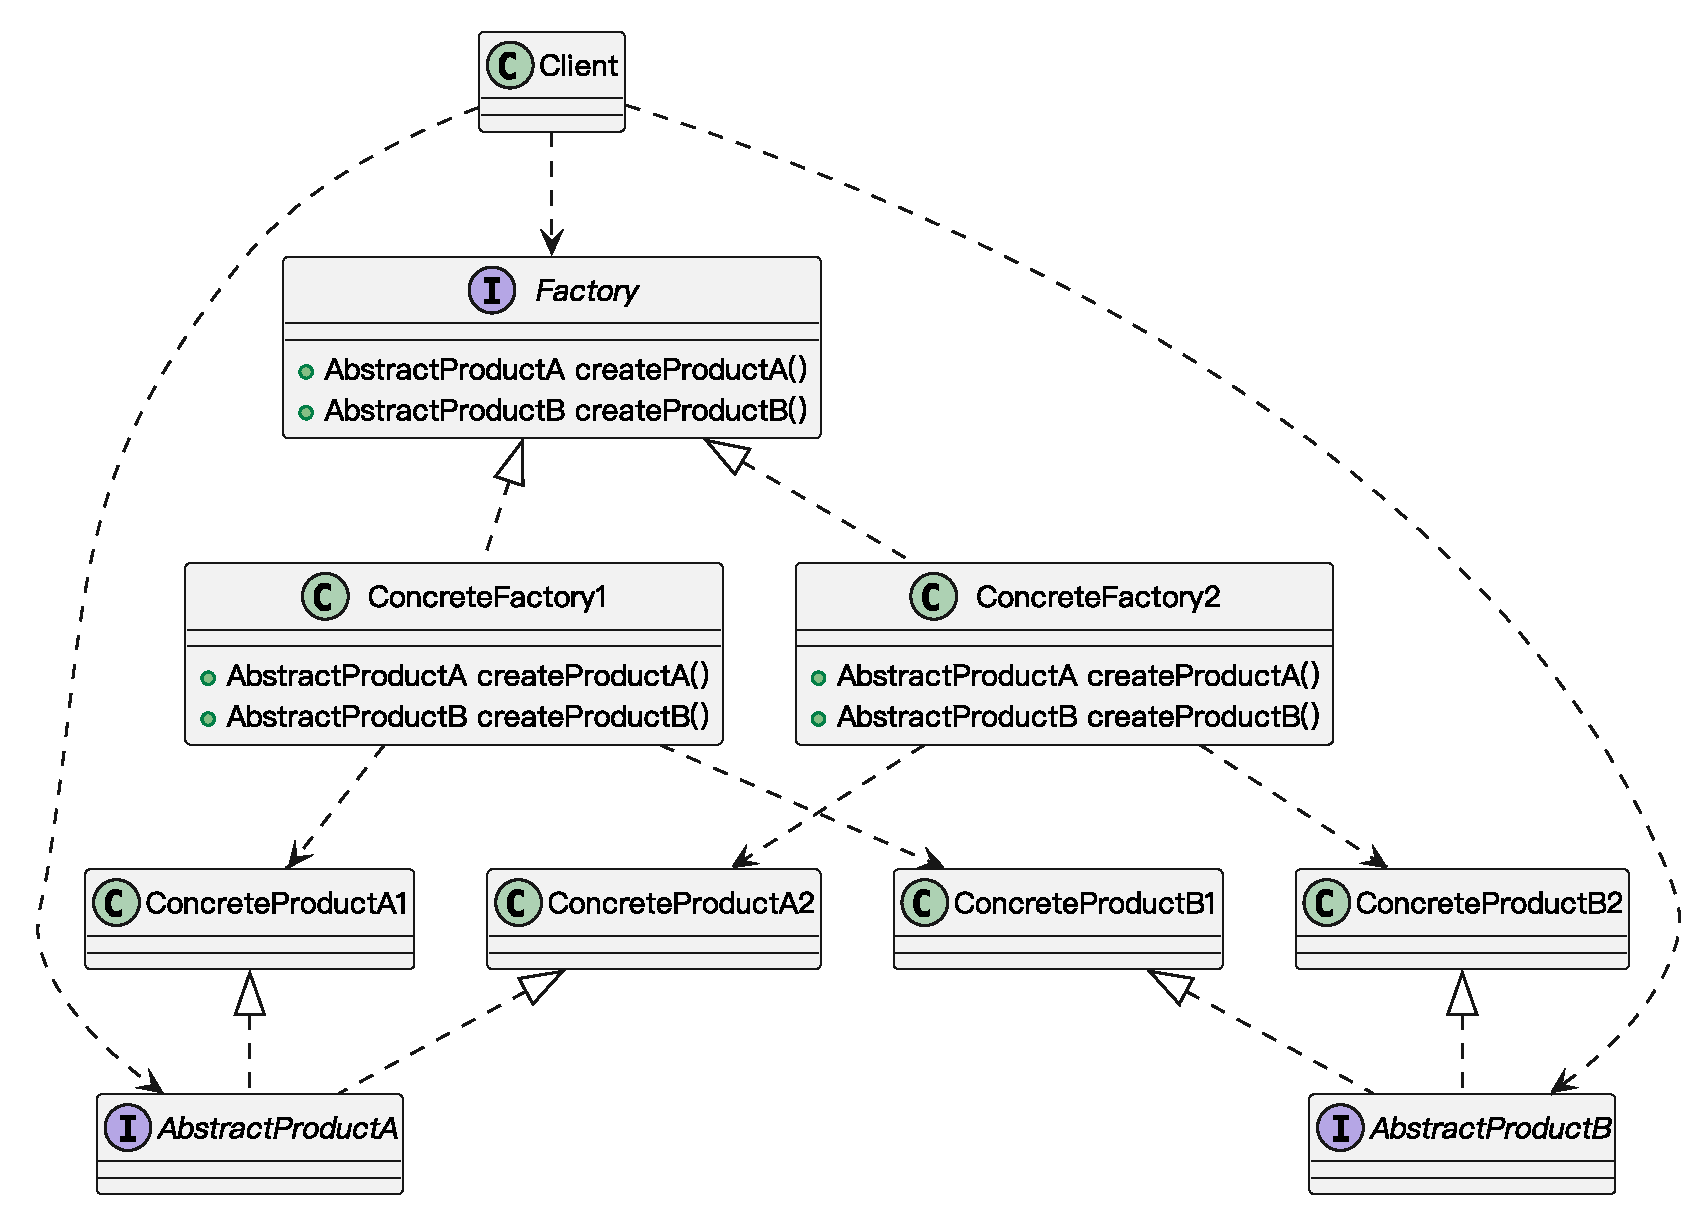
\includegraphics[width=0.8\textwidth]{images/抽象工厂模式.eps}
    \vspace{-1em}
\end{figure}

\begin{lstlisting}
public abstract class AbstractFactory {
    public abstract AbstractProductA createProductA();
    public abstract AbstractProductB createProductB();
}

public class ConcreteFactory1 extends AbstractFactory {
    public AbstractProductA createProductA() {
        return new ConcreteProductA1(); 
    }
    public AbstractProductB createProductB() {
        return new ConcreteProductB1(); 
    }
}
\end{lstlisting}

\subsubsection{模式分析}
如下图例,使用抽象工厂模式进行构建。
\begin{figure}[H]
    \vspace{-0.5em}
	\centering
	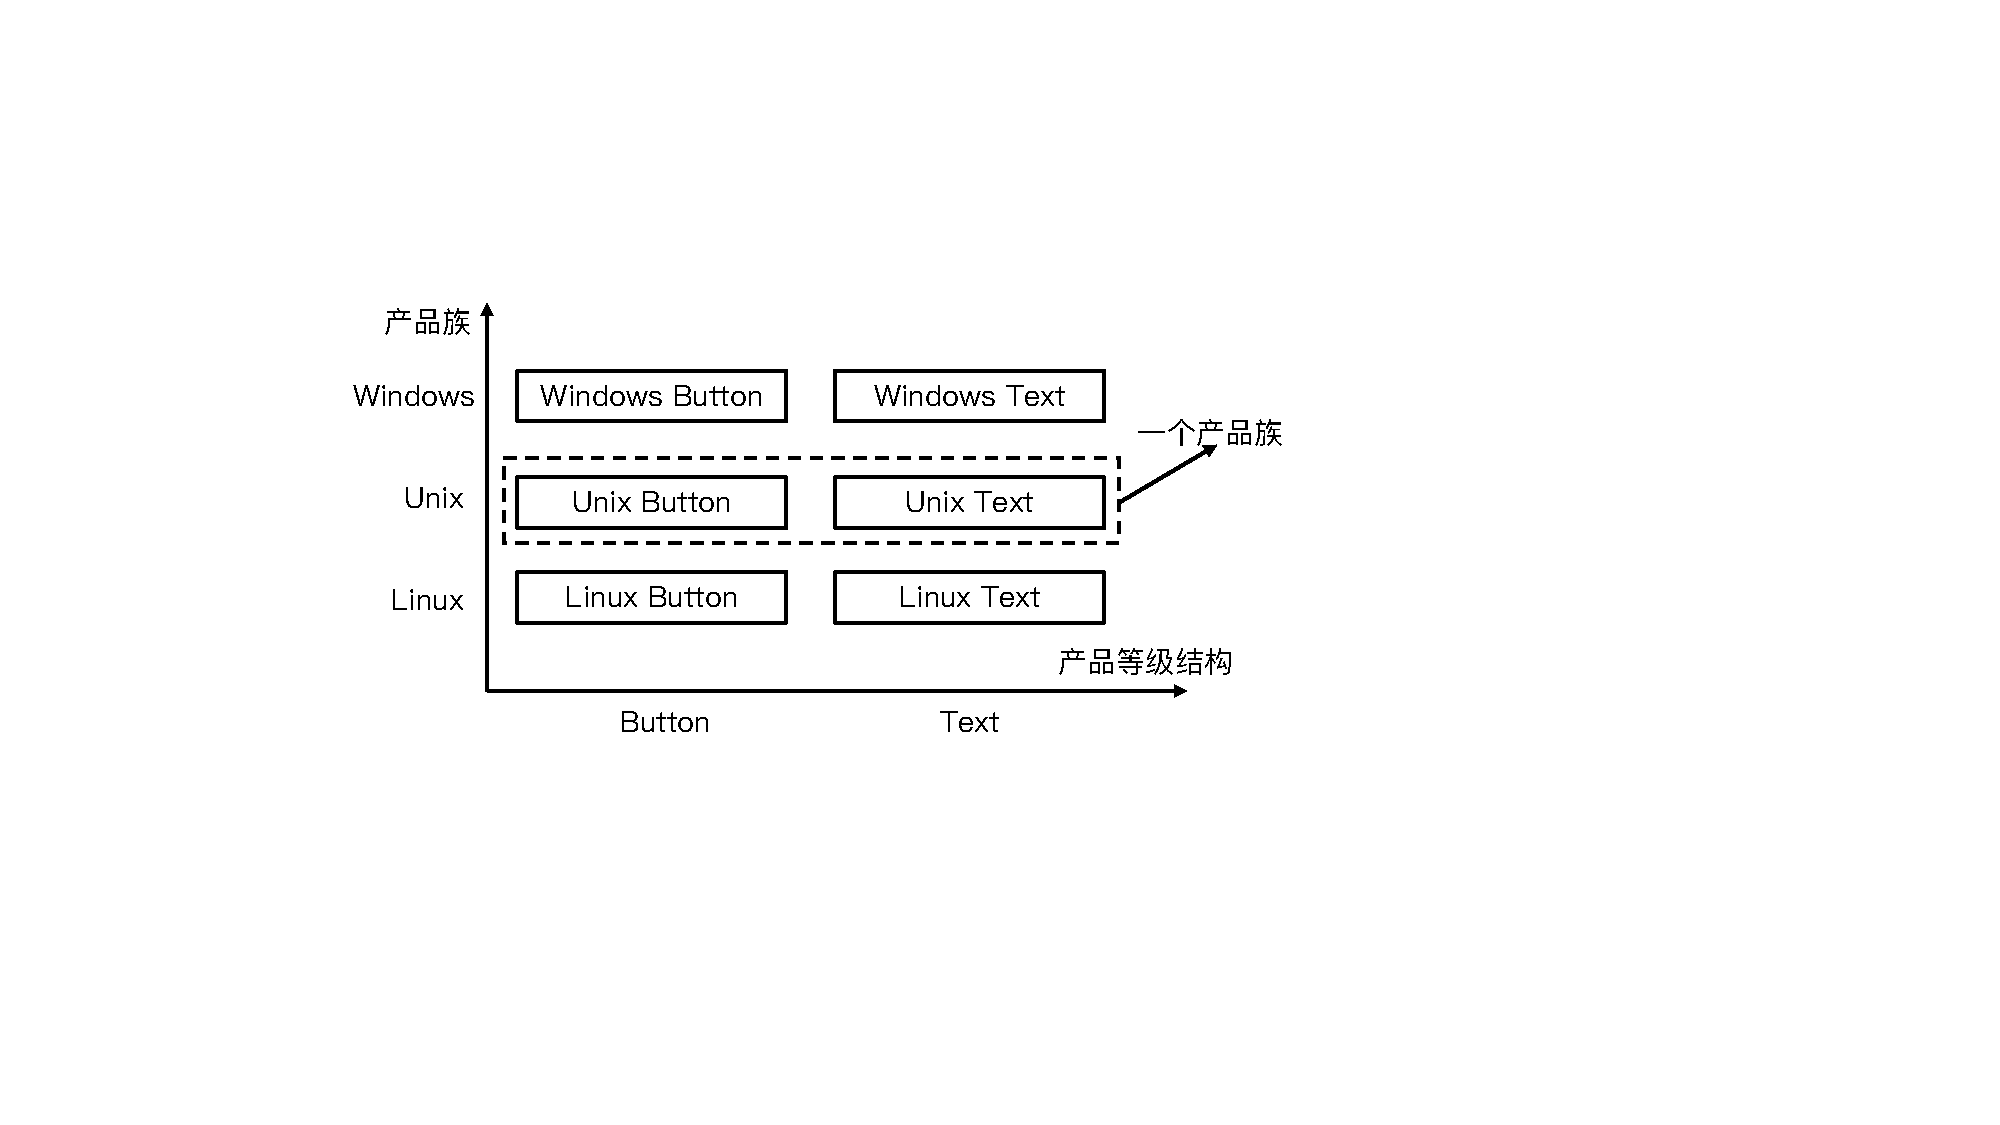
\includegraphics[width=0.5\textwidth]{images/抽象工厂模式分析.pdf}
    \vspace{-1em}
\end{figure}

\begin{figure}[H]
    \vspace{-0.5em}
	\centering
	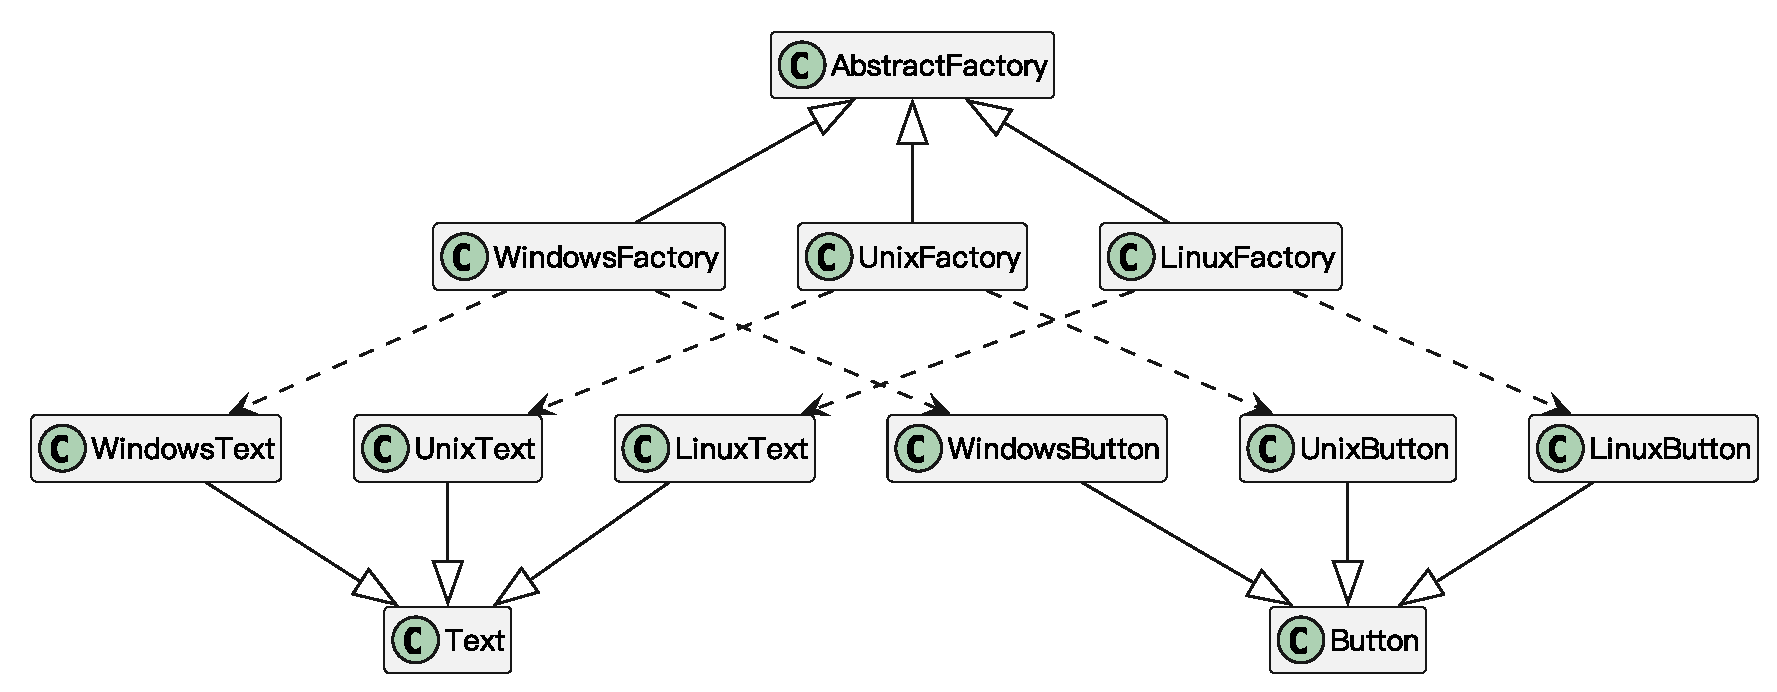
\includegraphics[width=0.73\textwidth]{images/抽象工厂模式分析.eps}
    \vspace{-1em}
\end{figure}

\subsubsection{模式实例}
电器工厂:一个电器工厂可以产生多种类型的电器,如海尔工厂可以生产海尔电视机、海尔空调等,TCL工厂可以生产TCL电视机、TCL空调等,相同品牌的电器构成一个产品族,而相同类型的电器构成了一个产品等级结构,现使用抽象工厂模式模拟该场景。
\begin{figure}[H]
    \vspace{-0.5em}
	\centering
	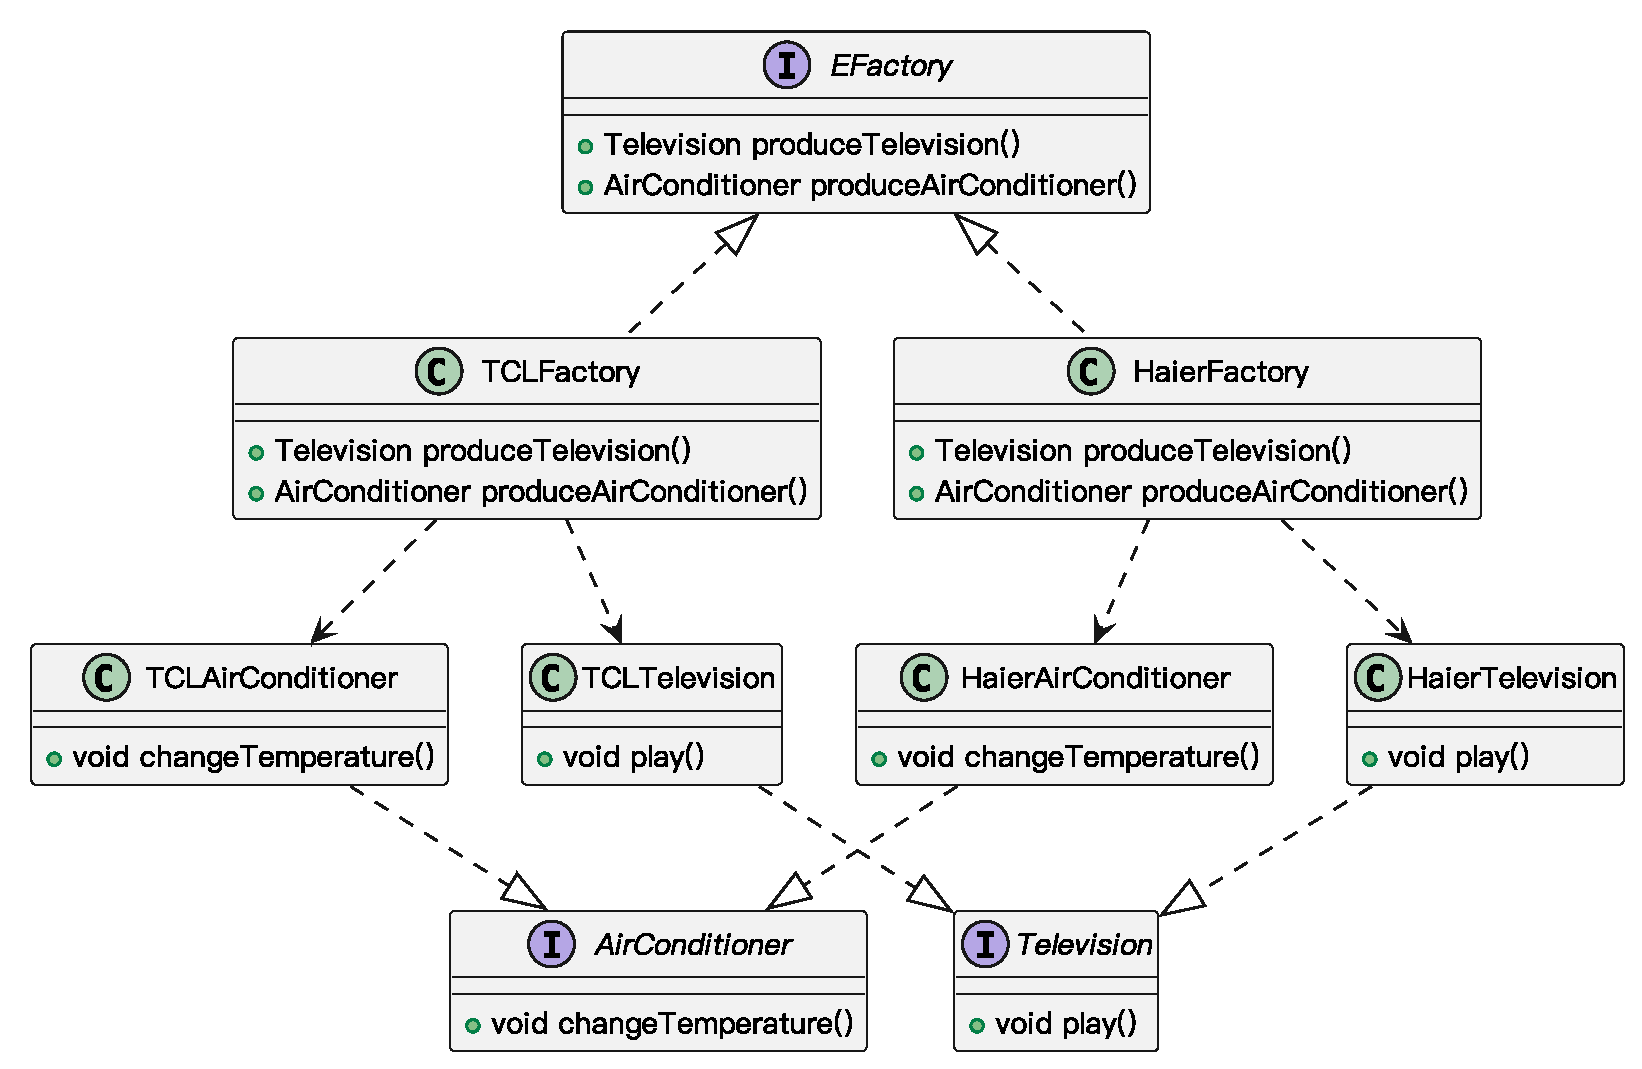
\includegraphics[width=0.7\textwidth]{images/抽象工厂模式实例1.eps}
    \vspace{-1em}
\end{figure}

据库操作工厂:某系统为了改进数据库操作的性能,自定义数据库连接对象Connection和语句对象Statement,可针对不同类型的数据库提供不同的连接对象和语句对象,如提供Oracle或SQL Server专用连接类和语句类,而且用户可以通过配置文件等方式根据实际需要动态更换系统数据库。使用抽象工厂模式设计该系统。
\begin{figure}[H]
    \vspace{-0.5em}
	\centering
	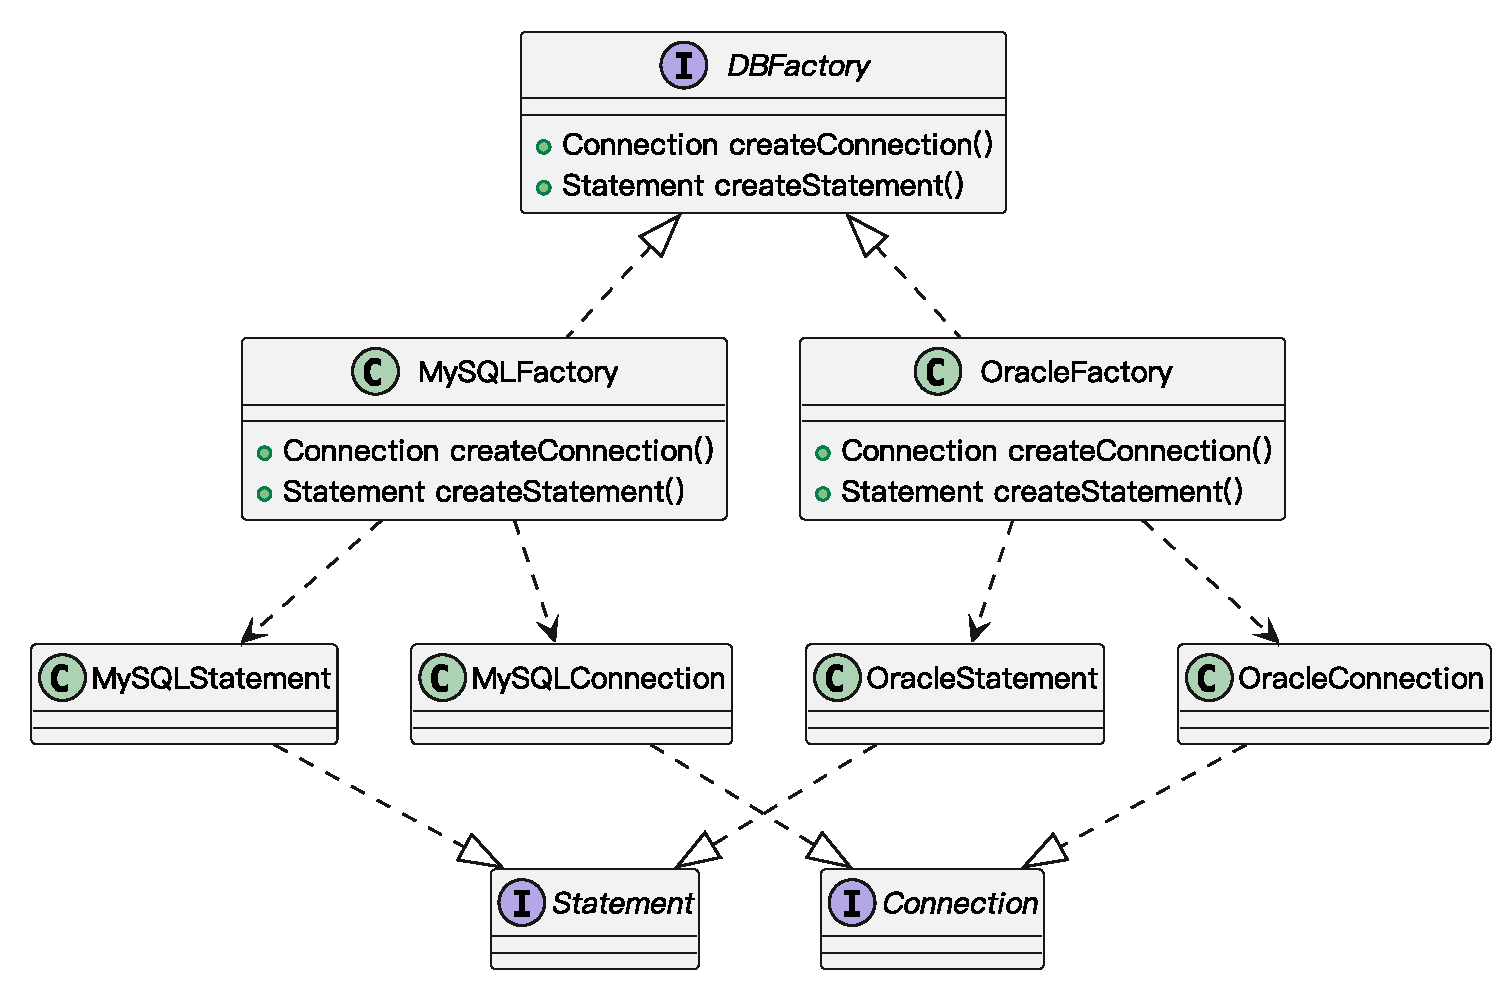
\includegraphics[width=0.67\textwidth]{images/抽象工厂模式实例2.eps}
    \vspace{-1em}
\end{figure}

\subsubsection{模式优缺点}
抽象工厂模式的优点:
\begin{itemize}
    \item 抽象工厂模式\textbf{隔离了具体类的生成},使得客户并不需要知道什么被创建。由于这种隔离,更换一个具体工厂就变得相对容易。所有的具体工厂都实现了抽象工厂中定义的那些公共接口,因此\textbf{只需改变具体工厂的实例,就可以在某种程度上改变整个软件系统的行为}。另外,应用抽象工厂模式\textbf{可以实现高内聚低耦合的设计目的},因此抽象工厂模式得到了广泛的应用。
    \item 当一个产品族中的多个对象被设计成一起工作时,它\textbf{能够保证客户端始终只使用同一个产品族中的对象}。这对一些需要根据当前环境来决定其行为的软件系统来说,是一种非常实用的设计模式。
    \item \textbf{增加新的具体工厂和产品族很方便,无须修改已有系统,符合“开闭原则”。}
\end{itemize}

抽象工厂模式的缺点:
\begin{itemize}
    \item 在添加新的产品对象时,\textbf{难以扩展抽象工厂来生产新种类的产品},这是因为在抽象工厂角色中规定了所有可能被创建的产品集合,要支持新种类的产品就意味着要对该接口进行扩展,而这将涉及到对抽象工厂角色及其所有子类的修改,显然会带来较大的不便。
    \item 上述缺点可概括为:\textbf{增加新的工厂和产品族容易,增加新的产品等级结构麻烦}(开闭原则的倾斜性)。
\end{itemize}

\subsubsection{模式适用环境}
在以下情况下可以使用抽象工厂模式:
\begin{itemize}
    \item 一个系统\textbf{不应当依赖于产品类实例如何被创建、组合和表达的细节},这对于所有类型的工厂模式都是重要的。
    \item 系统中\textbf{有多于一个的产品族},而每次只使用其中某一产品族。
    \item \textbf{属于同一个产品族的产品将在一起使用},这一约束必须在系统的设计中体现出来。
    \item 系统提供一个产品类的库,\textbf{所有的产品以同样的接口出现},从而使\textbf{客户端不依赖于具体实现}。
\end{itemize}

\subsubsection{模式扩展}
\paragraph*{“开闭原则”的倾斜性}~{} \par
“开闭原则”要求系统对扩展开放,对修改封闭,通过扩展达到增强其功能的目的。对于涉及到多个产品族与多个产品等级结构的系统,其功能增强包括两方面:
\begin{itemize}
    \item 增加产品族:\textbf{对于增加新的产品族,工厂方法模式很好的支持了“开闭原则”,对于新增加的产品族,只需要对应增加一个新的具体工厂即可,对已有代码无须做任何修改。}
    \item 增加新的产品等级结构:\textbf{对于增加新的产品等级结构,需要修改所有的工厂角色,包括抽象工厂类,在所有的工厂类中都需要增加生产新产品的方法,不能很好地支持“开闭原则”。}
\end{itemize}
抽象工厂模式的这种性质称为“开闭原则”的倾斜性,抽象工厂模式以一种倾斜的方式支持增加新的产品,它为新产品族的增加提供方便,但不能为新的产品等级结构的增加提供这样的方便。

\paragraph*{工厂模式的退化}~{} \par
当抽象工厂模式中每一个具体工厂类只创建一个产品对象,也就是\textbf{只存在一个产品等级结构时,抽象工厂模式退化成工厂方法模式};当\textbf{工厂方法模式中抽象工厂与具体工厂合并,提供一个统一的工厂来创建产品对象,并将创建对象的工厂方法设计为静态方法时,工厂方法模式退化成简单工厂模式}。

	\section{创建型模式}

\subsection{建造者模式}

\subsubsection{模式动机}
无论是在现实世界中还是在软件系统中,都存在一些复杂的对象,它们拥有多个组成部分,如汽车,它包括车轮、方向盘、发送机等各种部件。而对于大多数用户而言,无须知道这些部件的装配细节,也几乎不会使用单独某个部件,而是使用一辆完整的汽车,可以通过建造者模式对其进行设计与描述,\textbf{建造者模式可以将部件和其组装过程分开,一步一步创建一个复杂的对象}。用户只需要指定复杂对象的类型就可以得到该对象,而无须知道其内部的具体构造细节。

在软件开发中,也存在大量类似汽车一样的复杂对象,\textbf{它们拥有一系列成员属性,这些成员属性中有些是引用类型的成员对象}。而且在这些复杂对象中,还可能存在一些限制条件,如某些属性没有赋值则复杂对象不能作为一个完整的产品使用;有些属性的赋值必须按照某个顺序,一个属性没有赋值之前,另一个属性可能无法赋值等。

\textbf{复杂对象相当于一辆有待建造的汽车,而对象的属性相当于汽车的部件},建造产品的过程就相当于组合部件的过程。由于组合部件的过程很复杂,因此,这些部件的组合过程往往被“外部化”到一个称作建造者的对象里,\textbf{建造者返还给客户端的是一个已经建造完毕的完整产品对象,而用户无须关心该对象所包含的属性以及它们的组装方式},这就是建造者模式的模式动机。

\subsubsection{模式定义}
建造者模式(Builder Pattern):将一个复杂对象的构建与它的表示分离,使得同样的构建过程可以创建不同的表示。

建造者模式是\textbf{一步一步创建一个复杂的对象},它允许用户只通过指定复杂对象的类型和内容就可以构建它们,用户不需要知道内部的具体构建细节。建造者模式属于对象创建型模式。根据中文翻译的不同,建造者模式又可以称为生成器模式。

\subsubsection{模式结构}
建造者模式包含如下角色:
\vspace{-0.8em}
\begin{multicols}{2}
    \begin{itemize}
        \item Builder:抽象建造者
        \item ConcreteBuilder:具体建造者
        \item Director:指挥者
        \item Product:产品角色
    \end{itemize}
\end{multicols}
\vspace{-1em}

\begin{figure}[H]
    \vspace{-0.5em}
	\centering
	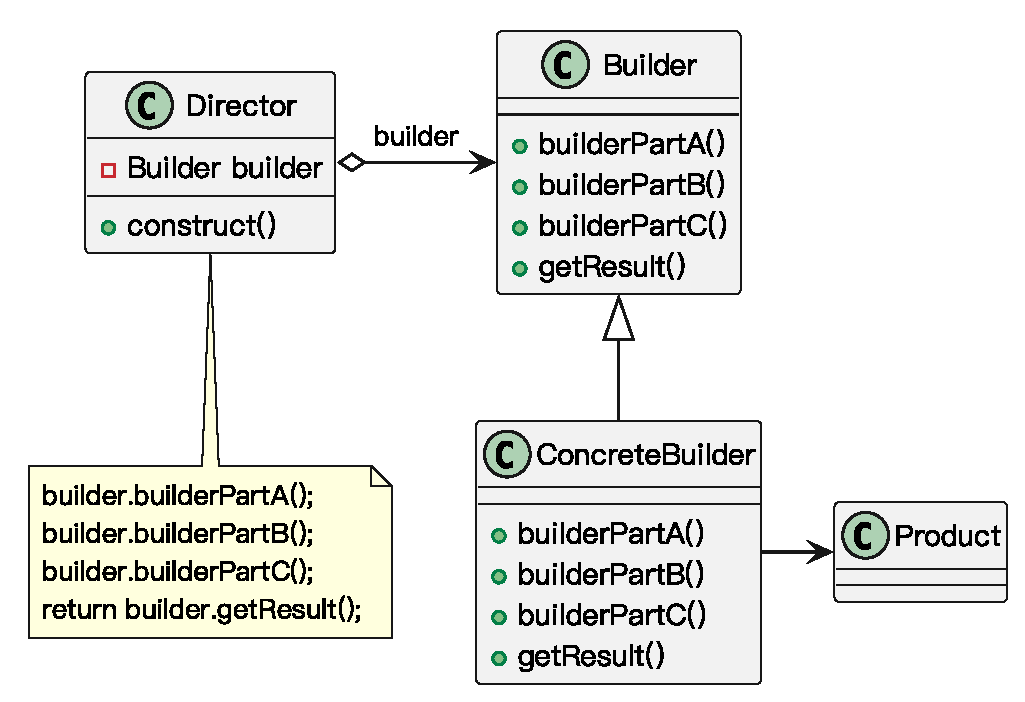
\includegraphics[width=0.55\textwidth]{images/建造者模式结构.eps}
    \vspace{-1em}
\end{figure}

\subsubsection{模式分析}
\begin{figure}[H]
    \vspace{-0.5em}
	\centering
	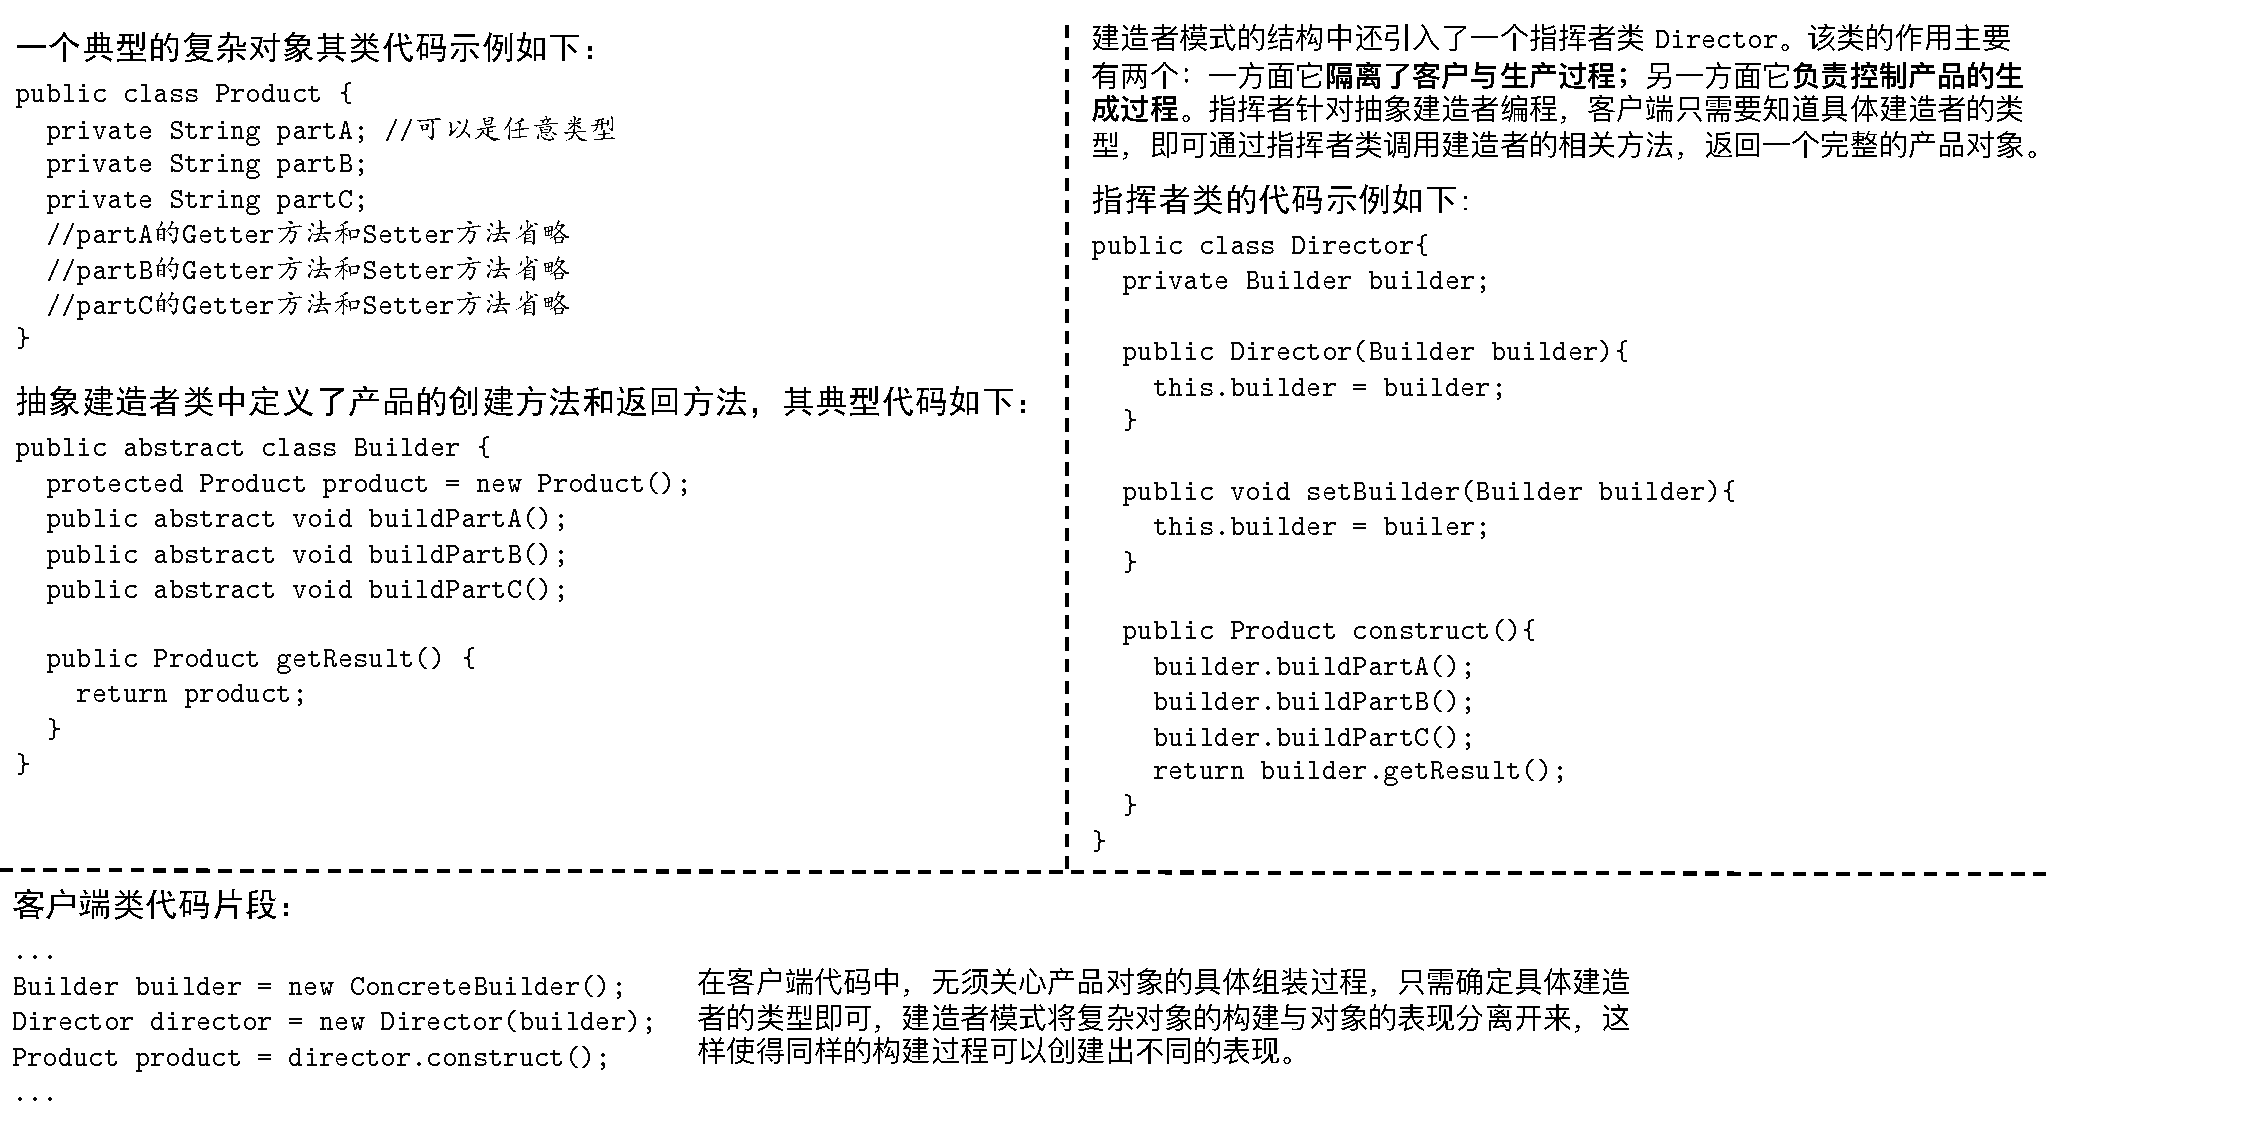
\includegraphics[width=\textwidth]{images/建造者模式分析.pdf}
    \vspace{-2em}
\end{figure}

\subsubsection{模式实例}
KFC套餐:建造者模式可以用于描述KFC如何创建套餐。套餐是一个复杂对象,它一般包含主食(如汉堡、鸡肉卷等)和饮料(如果汁、可乐等)等组成部分,不同的套餐有不同的组成部分,而KFC的服务员可以根据顾客的要求,一步一步装配这些组成部分,构造一份完整的套餐,然后返回给顾客。
\begin{figure}[H]
    \vspace{-0.5em}
	\centering
	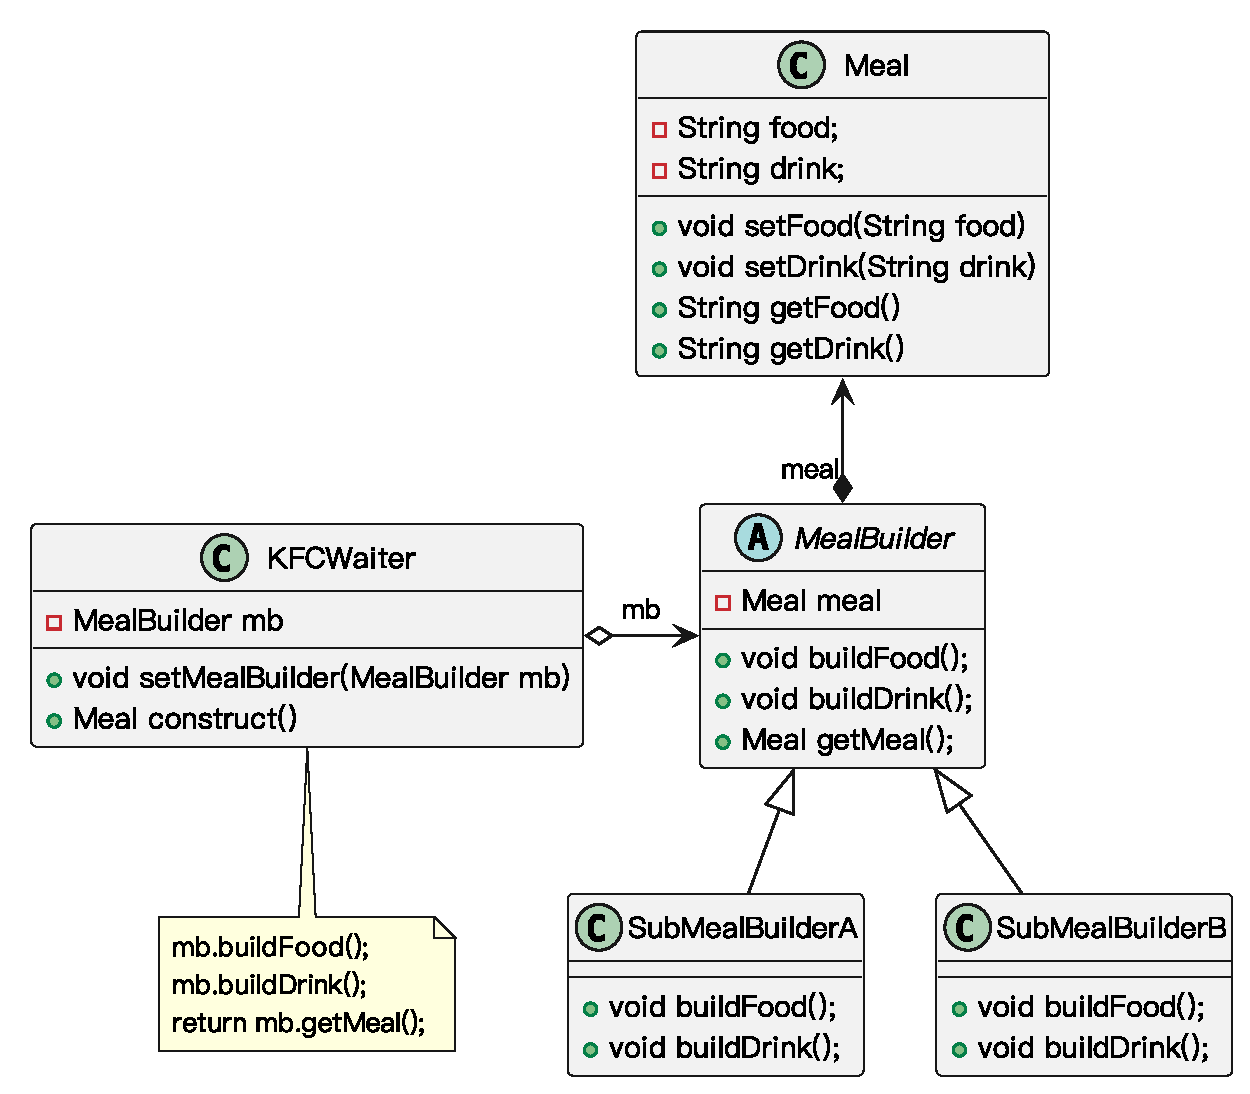
\includegraphics[width=0.6\textwidth]{images/建造者模式实例.eps}
    \vspace{-1em}
\end{figure}

\subsubsection{模式优缺点}
建造者模式的优点:
\begin{itemize}
    \item 在建造者模式中,\textbf{客户端不必知道产品内部组成的细节,将产品本身与产品的创建过程解耦,使得相同的创建过程可以创建不同的产品对象}。
    \item 每一个具体建造者都相对独立,而与其他的具体建造者无关,因此可以很方便地替换具体建造者或增加新的具体建造者,\textbf{用户使用不同的具体建造者即可得到不同的产品对象}。
    \item \textbf{可以更加精细地控制产品的创建过程}。将复杂产品的创建步骤分解在不同的方法中,使得创建过程更加清晰,也更方便使用程序来控制创建过程。
    \item \textbf{增加新的具体建造者无须修改原有类库的代码,指挥者类针对抽象建造者类编程,系统扩展方便,符合“开闭原则”。}
\end{itemize}

建造者模式的缺点:
\begin{itemize}
    \item 建造者模式所创建的产品一般具有较多的共同点,其组成部分相似,\textbf{如果产品之间的差异性很大,则不适合使用建造者模式,因此其使用范围受到一定的限制}。
    \item \textbf{如果产品的内部变化复杂,可能会导致需要定义很多具体建造者类来实现这种变化,导致系统变得很庞大。}
\end{itemize}

\subsubsection{模式适用环境}
在以下情况下可以使用建造者模式:
\begin{itemize}
    \item \textbf{需要生成的产品对象有复杂的内部结构},这些产品对象通常包含多个成员属性。
    \item \textbf{需要生成的产品对象的属性相互依赖,需要指定其生成顺序。}
    \item \textbf{对象的创建过程独立于创建该对象的类}。在建造者模式中引入了指挥者类,将创建过程封装在指挥者类中,而不在建造者类中。
    \item \textbf{隔离复杂对象的创建和使用,并使得相同的创建过程可以创建不同的产品。}
\end{itemize}

\subsubsection{模式应用}
\ding{172} JavaMail:一步一步构造一个完整的邮件对象,然后发送
\begin{lstlisting}
//由邮件会话对象新建一个邮件消息对象
MimeMessage message = new MimeMessage(session);
//设置邮件地址
InternetAddress from = new InternetAddress("sunny@test.com");
message.setFrom(from); //设置发件人
InternetAddress to = new InternetAddress(to_mail);
message.setRecipient(Message.RecipientType.TO,to); //设置收件人,并设置其接收类型为TO
message.setSubject(to_title); //设置主题
message.setText(to_content); //设置信件内容
message.setSentDate(new Date()); //设置发信时间
message.saveChanges(); //存储邮件信息
Transport transport = session.getTransport("smtp");
transport.connect("smtp.test.com","test","test");
transport.sendMessage(message,message.getAllRecipients());
\end{lstlisting}

\ding{173} 在很多游戏软件中,地图包括天空、地面、背景等组成部分,人物角色包括人体、服装、装备等组成部分,可以使用建造者模式对其进行设计,通过不同的具体建造者创建不同类型的地图或人物。

\subsubsection{建造者模式的简化}
\begin{itemize}
    \item \textbf{省略抽象建造者角色:}如果系统中只需要一个具体建造 者的话,可以省略掉抽象建造者。
    \item \textbf{省略指挥者角色:}在具体建造者只有一个的情况下,如果抽象建造者角色已经被省略掉,那么还可以省略指挥者角色,让\;\verb|Builder|\;角色扮演指挥者与建造者双重角色。
\end{itemize}

\subsubsection{建造者模式与抽象工厂模式的比较}
\begin{itemize}
    \item 与抽象工厂模式相比,建造者模式返回一个组装好的完整产品,而抽象工厂模式返回一系列相关的产品,这些产品位于不同的产品等级结构,构成了一个产品族。
    \item 在抽象工厂模式中,客户端实例化工厂类,然后调用工厂方法获取所需产品对象,而在建造者模式中,客户端可以不直接调用建造者的相关方法,而是通过指挥者类来指导如何生成对象,包括对象的组装过程和建造步骤,它侧重于一步步构造一个复杂对象,返回一个完整的对象。
    \item 如果将抽象工厂模式看成汽车配件生产工厂,生产一个产品族的产品,那么建造者模式就是一个汽车组装工厂,通过对部件的组装可以返回一辆完整的汽车。
\end{itemize}


\subsection{原型模式}

\subsubsection{模式动机}
\begin{itemize}
    \item 在面向对象系统中,使用原型模式来复制一个对象自身,从而\textbf{克隆出多个与原型对象一模一样的对象}。
    \item 在软件系统中,有些对象的创建过程较为复杂,而且有时候需要频繁创建,\textbf{原型模式通过给出一个原型对象来指明所要创建的对象的类型,然后用复制这个原型对象的办法创建出更多同类型的对象},这就是原型模式的意图所在。
\end{itemize}

\subsubsection{模式定义}
原型模式(Prototype Pattern):原型模式是一种对象创建型模式,\textbf{用原型实例指定创建对象的种类,并且通过复制这些原型创建新的对象}。原型模式允许一个对象再创建另外一个可定制的对象,无须知道任何创建的细节。

原型模式的基本工作原理是通过将一个原型对象传给那个要发动创建的对象,这个要发动创建的对象通过请求原型对象拷贝原型自己来实现创建过程。

\subsubsection{模式结构}
原型模式包含如下角色:
\vspace{-0.8em}
\begin{multicols}{2}
    \begin{itemize}
        \item Prototype:抽象原型类
        \item ConcretePrototype:具体原型类
        \item Client:客户类
    \end{itemize}
\end{multicols}
\vspace{-1em}

\begin{figure}[H]
    \vspace{-0.5em}
	\centering
	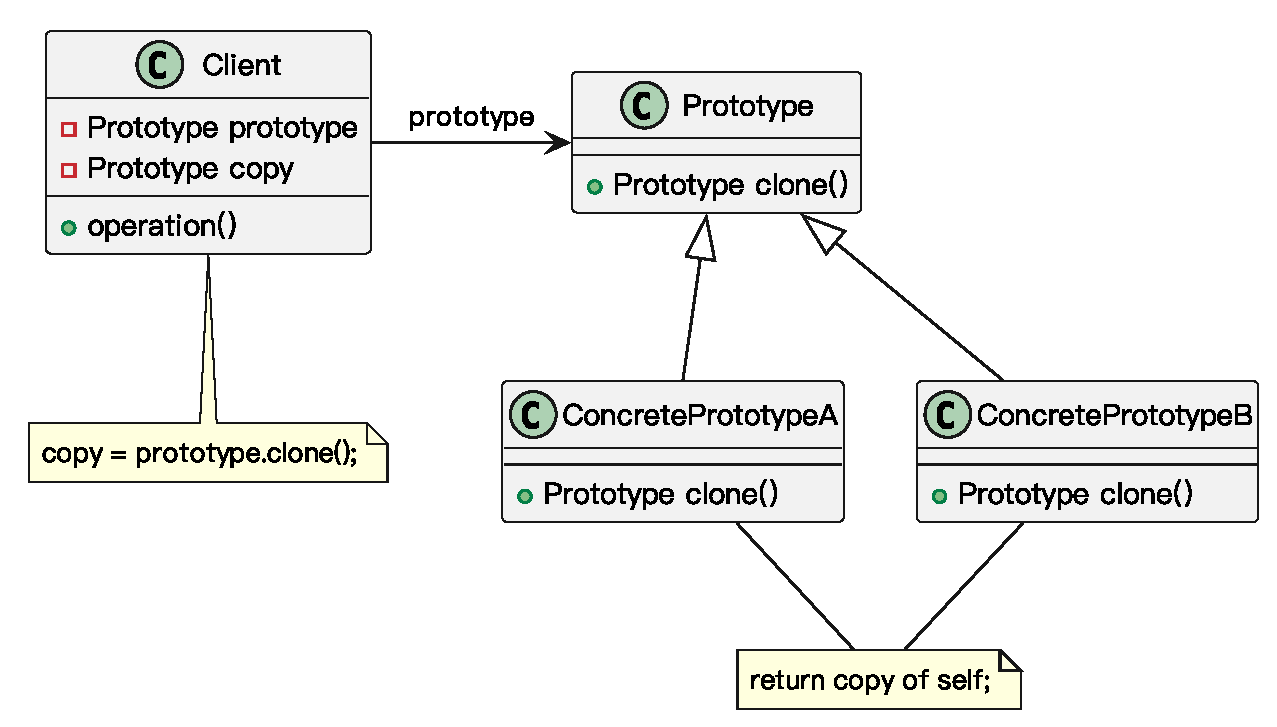
\includegraphics[width=0.6\textwidth]{images/原型模式结构.eps}
    \vspace{-1em}
\end{figure}

\subsubsection{模式分析}
\begin{itemize}
    \item 在原型模式结构中定义了一个抽象原型类,所有的Java类都继承自\;\verb|java.lang.Object|,而\;\verb|Object|类提供一个\;\verb|clone()|\;方法,可以将一个Java对象复制一份。因此在Java中可以直接使用\;\verb|Object|\;提供的\;\verb|clone()|\;方法来实现对象的克隆,Java语言中的原型模式实现很简单。
    \item 能够实现克隆的Java类必须实现一个标识接口\;\verb|Cloneable|,表示这个Java类支持复制。如果一个类没有实现这个接口但是调用了\verb|clone()|方法,Java编译器将抛出一个\verb|CloneNotSupportedException| 异常。
    \begin{lstlisting}
public class PrototypeDemo implements Cloneable {
...
    public Object clone() {
        Object object = null; 
        try {
            object = super.clone();
        } catch (CloneNotSupportedException exception) { 
            System.err.println("Not support cloneable");
        }
        return object; 
    }
...
}
    \end{lstlisting}
    \item 通常情况下,一个类包含一些成员对象,在使用原型模式克隆对象时,根据其成员对象是否也克隆,原型模式可以分为两种形式:\textbf{深克隆}和\textbf{浅克隆}。
\end{itemize}

\vspace{-0.5em}
\begin{shaded}
Java语言提供的\;\verb|clone()|\;方法将对象复制了一份并返回给调用者。一般而言,\;\verb|clone()|\;方法满足:
\begin{enumerate}[label=(\arabic*)]
    \item 对任何的对象\;\verb|x|,都有\;\verb|x.clone() != x|,即克隆对象与原对象不是同一个对象。
    \item 对任何的对象\;\verb|x|,都有\;\verb|x.clone().getClass() == x.getClass()|,即克隆对象与原对象的类型一样。
    \item 如果对象\;\verb|x|\;的\;\verb|equals()|\;方法定义恰当,那么\;\verb|x.clone().equals(x)|\;应该成立。
\end{enumerate}
\end{shaded}
\vspace{-1em}

\subsubsection{模式实例}
邮件复制(浅克隆):由于邮件对象包含的内容较多(如发送者、接收者、标题、内容、日期、附件等),某系统中现需要提供一个邮件复制功能,对于已经创建好的邮件对象,可以通过复制的方式创建一个新的邮件对象,如果需要改变某部分内容,无须修改原始的邮件对象,只需要修改复制后得到的邮件对象即可。使用原型模式设计该系统。在本实例中使用浅克隆实现邮件复制,即复制邮件(Email)的同时不复制附件(Attachment)。
\begin{figure}[H]
    \vspace{-0.5em}
	\centering
	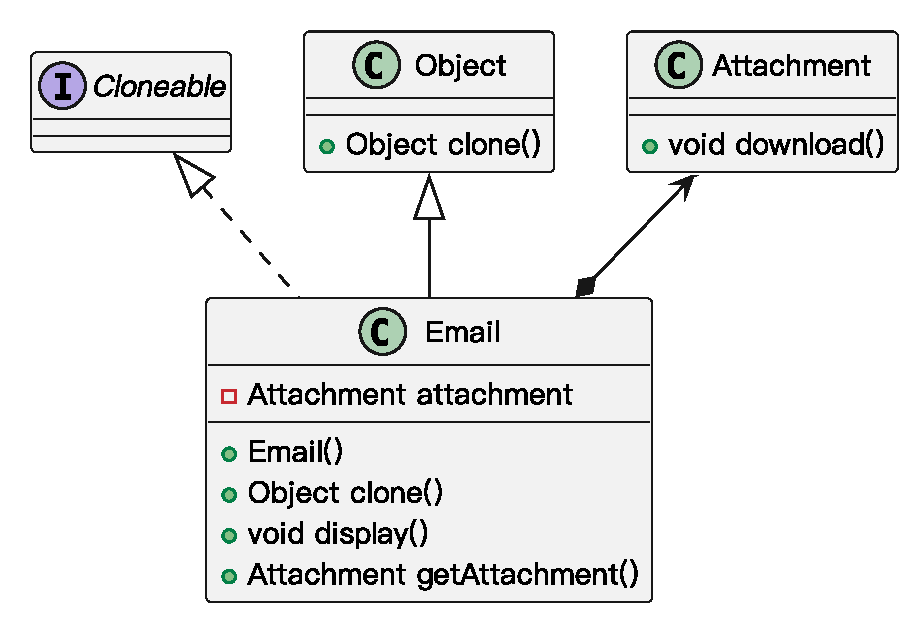
\includegraphics[width=0.4\textwidth]{images/原型模式实例.eps}
    \vspace{-1em}
\end{figure}

\subsubsection{模式优缺点}
原型模式的优点:
\begin{itemize}
    \item 当创建新的对象实例较为复杂时,使用原型模式可以\textbf{简化对象的创建过程},通过一个已有实例可以\textbf{提高新实例的创建效率}。
    \item 可以\textbf{动态增加或减少产品类}。
    \item 原型模式提供了\textbf{简化的创建结构}。
    \item 可以使用深克隆的方式\textbf{保存对象的状态}。
\end{itemize}

原型模式的缺点:
\begin{itemize}
    \item \textbf{需要为每一个类配备一个克隆方法},而且这个克隆方法需要对类的功能进行通盘考虑,这对全新的类来说不是很难,但对已有的类进行改造时,不一定是件容易的事,必须修改其源代码,违背了“开闭原则”。
    \item \textbf{在实现深克隆时需要编写较为复杂的代码}。
\end{itemize}

\subsubsection{模式适用环境}
在以下情况下可以使用原型模式:
\begin{itemize}
    \item \textbf{创建新对象成本较大},新的对象可以通过原型模式对已有对象进行复制来获得,如果是相似对象,则可以对其属性稍作修改。
    \item 如果\textbf{系统要保存对象的状态},而对象的状态变化很小,或者对象本身占内存不大的时候,也可以使用原型模式配合备忘录模式来应用。相反,如果对象的状态变化很大,或者对象占用的内存很大,那么采用状态模式会比原型模式更好。
    \item 需要\textbf{避免使用分层次的工厂类来创建分层次的对象},并且类的实例对象只有一个或很少的几个组合状态,通过复制原型对象得到新实例可能比使用构造函数创建一个新实例更加方便。
\end{itemize}

\subsubsection{模式应用}
\ding{172} 原型模式应用于很多软件中,如果每次创建一个对象要花大量时间,原型模式是最好的解决方案。很多软件提供的\textbf{复制}和\textbf{粘贴}操作就是原型模式的应用,复制得到的对象与原型对象是两个类型相同但内存地址不同的对象,通过原型模式可以大大提高对象的创建效率。

\ding{173} 在Struts2中为了保证线程的安全性,Action对象的创建使用了原型模式,访问一个已经存在的Action对象时将通过克隆的方式创建出一个新的对象,从而保证其中定义的变量无须进行加锁实现同步,每一个Action中都有自己的成员变量,避免Struts1因使用单例模式而导致的并发和同步问题。

\ding{174} 在Spring中,用户也可以采用原型模式来创建新的bean实例,从而实现每次获取的是通过克隆生成的新实例,对其进行修改时对原有实例对象不造成任何影响。

\subsubsection{模式扩展}

\paragraph*{相似对象的复制}~{} \par
很多情况下,复制所得到的对象与原型对象并不是完全相同的,它们的某些属性值存在异同。\textbf{通过原型模式获得相同对象后可以再对其属性进行修改,从而获取所需对象}。如多个学生对象的信息的区别在于性别、姓名和年龄,而专业、学院、学校等信息都相同,为了简化创建过程,可以通过原型模式来实现相似对象的复制。

\paragraph*{带原型管理器的原型模式}~{} \par
\begin{figure}[H]
    \vspace{-0.5em}
	\centering
	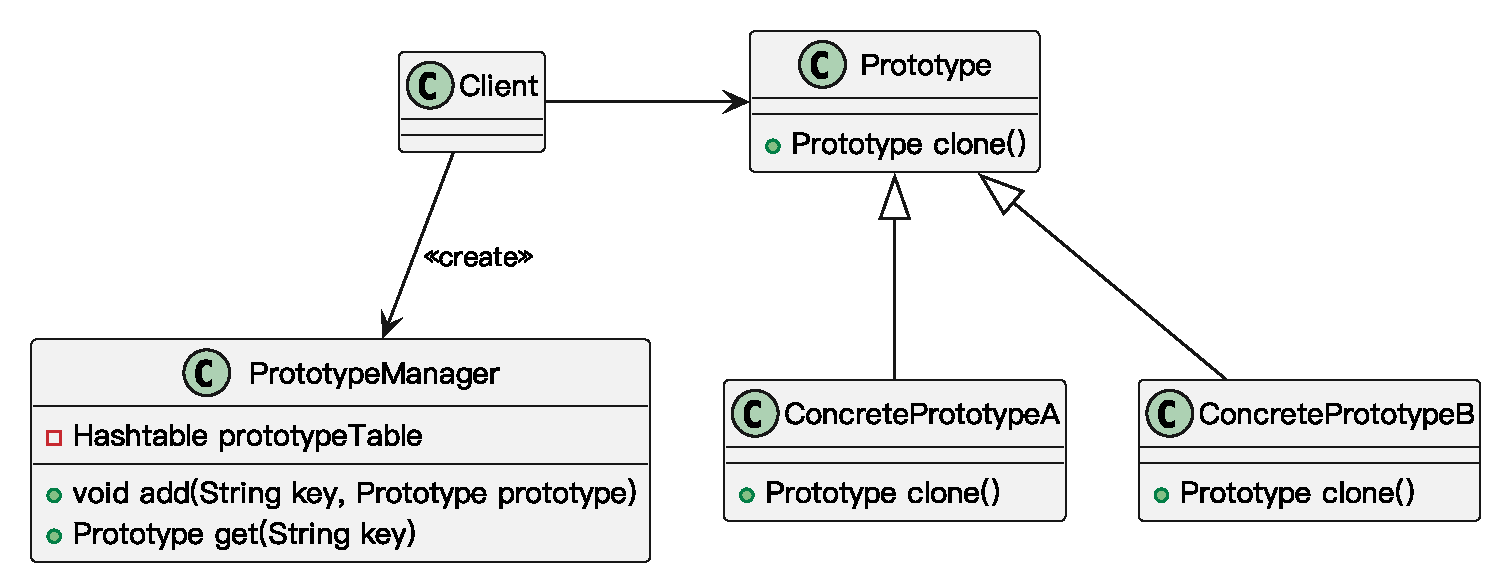
\includegraphics[width=0.8\textwidth]{images/原型模式拓展.eps}
    \vspace{-1em}
\end{figure}
	\section{状态与命令模式}

\subsection{状态模式}

\subsubsection{模式动机}
在很多情况下,\textbf{一个对象的行为取决于一个或多个动态变化的属性},这样的属性叫做\textbf{状态},这样的对象叫做有状态的(stateful)对象,这样的对象状态是从事先定义好的一系列值中取出的。当一个这样的对象与外部事件产生互动时,其内部状态就会改变 ,从而使得系统的行为也随之发生变化。

\subsubsection{模式定义}
状态模式(State Pattern):允许一个对象在其内部状态改变时改变它的行为,对象看起来似乎修改了它的类。其别名为状态对象(Objects for States),状态模式是一种对象行为型模式。

\subsubsection{模式结构}
状态模式包含如下角色:
\vspace{-0.8em}
\begin{multicols}{3}
    \begin{itemize}
        \item Context:环境类
        \item State:抽象状态类
        \item ConcreteState:具体状态类
    \end{itemize}
\end{multicols}
\vspace{-1em}

\begin{figure}[H]
    \vspace{-0.5em}
	\centering
	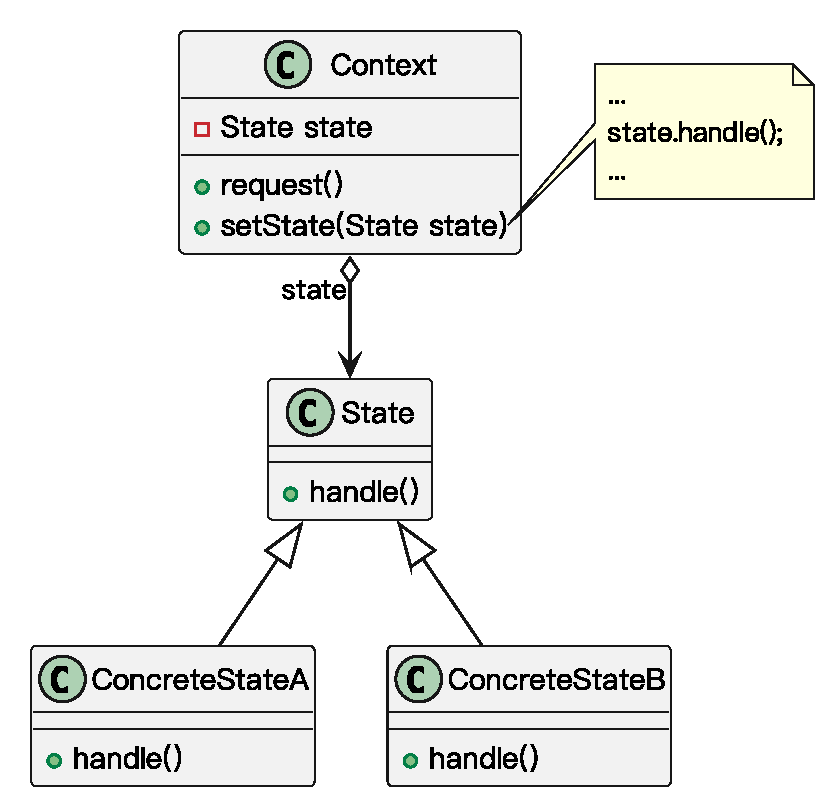
\includegraphics[width=0.42\textwidth]{images/状态模式结构.eps}
    \vspace{-1em}
\end{figure}

\subsubsection{模式分析}
\begin{figure}[H]
    \vspace{-0.5em}
	\centering
	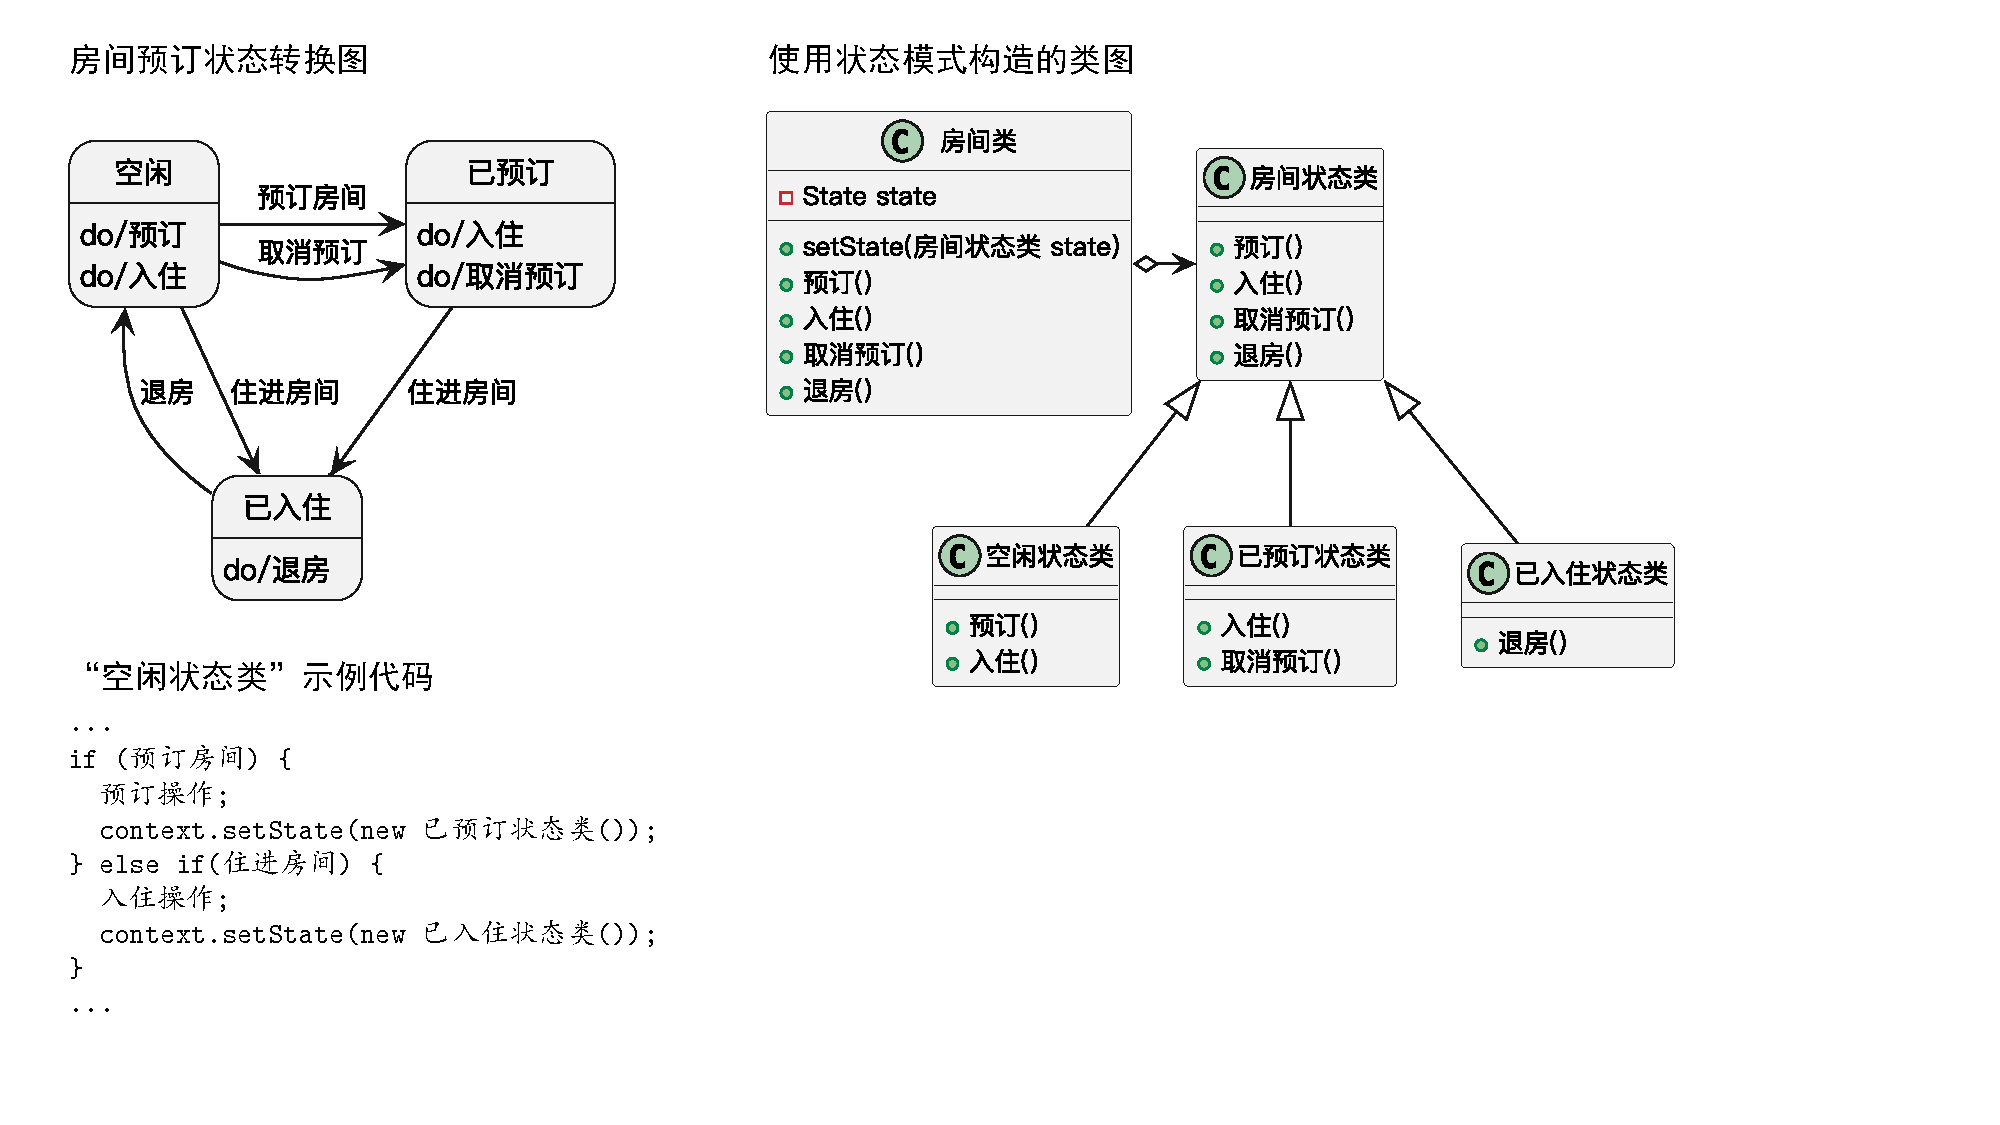
\includegraphics[width=0.7\textwidth]{images/状态模式分析.pdf}
    \vspace{-1em}
\end{figure}

\begin{itemize}
    \item 状态模式描述了对象状态的变化以及对象如何在每一种状态下表现出不同的行为。
    \item 状态模式的关键是引入了一个抽象类来专门表示对象的状态,这个类我们叫做抽象状态类,而对象的每一种具体状态类都继承了该类,并在不同具体状态类中实现了不同状态的行为,包括各种状态之间的转换。
\end{itemize}

在状态模式结构中需要理解\textbf{环境类}与\textbf{抽象状态类}的作用:
\begin{itemize}
    \item 环境类实际上就是\textbf{拥有状态的对象},环境类有时候可以充当状态管理器(State Manager)的角色,\textbf{可以在环境类中对状态进行切换操作}。
    \item 抽象状态类可以是抽象类,也可以是接口,不同状态类就是继承这个父类的不同子类,状态类的产生是由于环境类存在多个状态,同时还满足两个条件:这些状态经常需要切换,在不同的状态下对象的行为不同。因此可以\textbf{将不同对象下的行为单独提取出来封装在具体的状态类中,使得环境类对象在其内部状态改变时可以改变它的行为,对象看起来似乎修改了它的类,而实际上是由于切换到不同的具体状态类实现的}。由于环境类可以设置为任一具体状态类,因此它针对抽象状态类进行编程,在程序运行时可以将任一具体状态类的对象设置到环境类中,从而使得环境类可以改变内部状态,并且改变行为。
\end{itemize}

\subsubsection{模式实例}
论坛用户等级:在某论坛系统中,用户可以发表留言,发表留言将增加积分;用户也可以回复留言,回复留言也将增加积分;用户还可以下载文件,下载文件将扣除积分。该系统用户分为三个等级,分别是新手、高手和专家,这三个等级对应三种不同的状态,这三种状态分别定义如下
\begin{enumerate}[label=(\arabic*)]
    \item 如果积分小于100分,则为新手状态,用户可以发表留言、回复留言,但是不能下载文件。如果积分大于等于1000分,则转换为专家状态;如果积分大于等于100分,则转换为高手状态。
    \item 如果积分大于等于100分但小于1000分,则为高手状态,用户可以发表留言、回复留言,还可以下载文件,而且用户在发表留言时可以获取双倍积分。如果积分小于100分,则转换为新手状态;如果积分大于等于1000分,则转换为专家状态;如果下载文件后积分小于0,则不能下载该文件。
    \item 如果积分大于等于1000分,则为专家状态,用户可以发表留言、回复留言和下载文件,用户除了在发表留言时可以获取双倍积分外,下载文件只扣除所需积分的一半。如果积分小于100分,则转换为新手状态;如果积分小于1000分,但大于等于100,则转换为高手状态;如果下载文件后积分小于0,则不能下载该文件。
\end{enumerate}
\begin{figure}[H]
    \vspace{-0.5em}
	\centering
	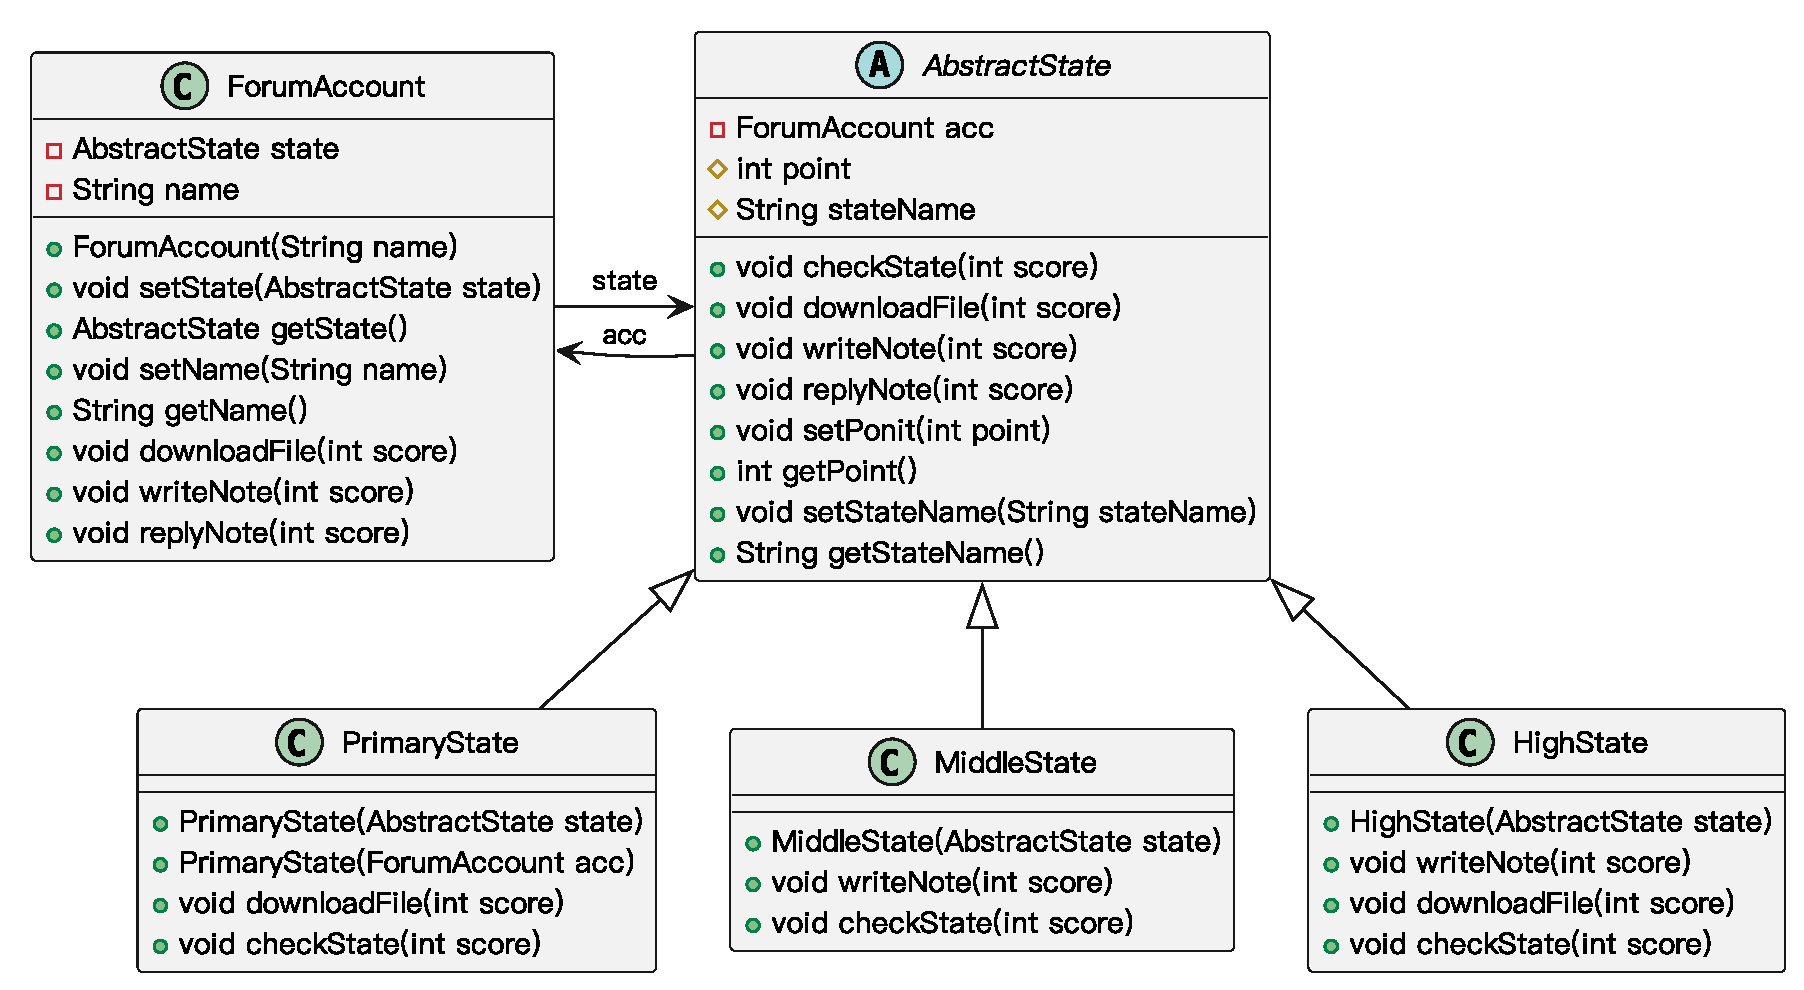
\includegraphics[width=0.8\textwidth]{images/状态模式实例.eps}
    \vspace{-1em}
\end{figure}

\subsubsection{模式优缺点}
状态模式的优点:
\begin{itemize}
    \item \textbf{封装了转换规则}。
    \item \textbf{枚举可能的状态},在枚举状态之前需要确定状态种类。
    \item 将所有与某个状态有关的行为放到一个类中,并且\textbf{可以方便地增加新的状态},只需要改变对象状态即可改变对象的行为。
    \item 允许\textbf{状态转换逻辑与状态对象合成一体},而不是某一个巨大的条件语句块。
    \item 可以\textbf{让多个环境对象共享一个状态对象},从而减少系统中对象的个数。
\end{itemize}

状态模式的缺点:
\begin{itemize}
    \item 状态模式的使用必然会\textbf{增加系统类和对象的个数}。
    \item 状态模式的结构与实现都较为复杂,\textbf{如果使用不当将导致程序结构和代码的混乱}。
    \item 状态模式\textbf{对“开闭原则”的支持并不太好},对于可以切换状态的状态模式,增加新的状态类需要修改那些负责状态转换的源代码,否则无法切换到新增状态;而且修改某个状态类的行为也需修改对应类的源代码。
\end{itemize}

\subsubsection{模式适用环境}
在以下情况下可以使用状态模式:
\begin{itemize}
    \item 对象的\textbf{行为依赖于它的状态(属性)}并且可以\textbf{根据它的状态改变而改变它的相关行为}。
    \item 代码中\textbf{包含大量与对象状态有关的条件语句},这些条件语句的出现,会导致代码的可维护性和灵活性变差,不能方便地增加和删除状态,使客户类与类库之间的耦合增强。在这些条件语句中包含了对象的行为,而且这些条件对应于对象的各种状态。
\end{itemize}

\subsubsection{模式应用}
\ding{172} 状态模式在\textbf{工作流}或\textbf{游戏}等类型的软件中得以广泛使用,甚至可以用于这些系统的核心功能设计,如在政府OA办公系统中,一个批文的状态有多种:尚未办理、正在办理、正在批示、正在审核、已经完成等各种状态,而且批文状态不同时对批文的操作也有所差异。\textbf{使用状态模式可以描述工作流对象(如批文)的状态转换以及不同状态下它所具有的行为}。

\ding{173} 在目前主流的RPG(角色扮演游戏)中,\textbf{使用状态模式可以对游戏角色进行控制},游戏角色的升级伴随着其状态的变化和行为的变化。对于游戏程序本身也可以通过状态模式进行总控,一个游戏活动包括开始、运行、结束等状态,通过对状态的控制可以控制系统的行为,决定游戏的各个方面,因此\textbf{可以使用状态模式对整个游戏的架构进行设计与实现}。

\subsubsection{模式扩展}

\paragraph*{共享状态}~{} \par
在有些情况下\textbf{多个环境对象需要共享同一个状态},如果希望在系统中实现多个环境对象实例共享一个或多个状态对象,那么\textbf{需要将这些状态对象定义为环境的静态成员对象}。

\paragraph*{简单状态模式}~{} \par
简单状态模式是指状态都相互独立,状态之间无须进行转换的状态模式,这是最简单的一种状态模式。
\begin{itemize}
    \item 对于这种状态模式,每个状态类都封装与状态相关的操作,而无须关心状态的切换,可以在客户端 直接实例化状态类,然后将状态对象设置到环境类中。
    \item 如果是这种简单的状态模式,它遵循“开闭原则”,在客户端可以针对抽象状态类进行编程,而将具体状态类写到配置文件中,同时增加新的状态类对原有系统也不造成任何影响。
\end{itemize} 

\paragraph*{可切换状态的状态模式}~{} \par
大多数的状态模式都是可以切换状态的状态模式
\begin{itemize}
    \item 在实现状态切换时,在具体状态类内部需要调用环境类\;\verb|Context的setState()|\;方法进行状态的转换操作,在具体状态类中可以调用到环境类的方法,因此状态类与环境类之间通常还存在关联关系或者依赖关系。
    \item 通过在状态类中引用环境类的对象来回调环境类的\;\verb|setState()|\;方法实现状态的切换。
    \item 在这种可以切换状态的状态模式中,增加新的状态类可能需要修改其他某些状态类甚至环境类的源代码,否则系统无法切换到新增状态。
\end{itemize}


\subsection{命令模式}

\subsubsection{模式动机}
在软件设计中,我们经常需要向某些对象发送请求,但是并不知道请求的接收者是谁,也不知道被请求的操作是哪个,我们只需在程序运行时指定具体的请求接收者即可,此时可以使用命令模式来进行设计,\textbf{使得请求发送者与请求接收者消除彼此之间的耦合},让对象之间的调用关系更加灵活。

命令模式可以对发送者和接收者完全解耦,发送者与接收者之间没有直接引用关系,\textbf{发送请求的对象只需要知道如何发送请求,而不必知道如何完成请求}。这就是命令模式的模式动机。

\subsubsection{模式定义}
命令模式(Command Pattern):将一个请求封装为一个对象,从而使我们可用不同的请求对客户进行参数化;对请求排队或者记录请求日志,以及支持可撤销的操作。命令模式是一种对象行为型模式,其别名为动作(Action)模式或事务(Transaction)模式。

\subsubsection{模式结构}
命令模式包含如下角色:
\vspace{-0.8em}
\begin{multicols}{2}
    \begin{itemize}
        \item Command: 抽象命令类
        \item ConcreteCommand: 具体命令类
        \item Invoker: 调用者
        \item Receiver: 接收者
        \item Client:客户类
    \end{itemize}
\end{multicols}
\vspace{-1em}
\begin{figure}[H]
    \vspace{-0.5em}
	\centering
	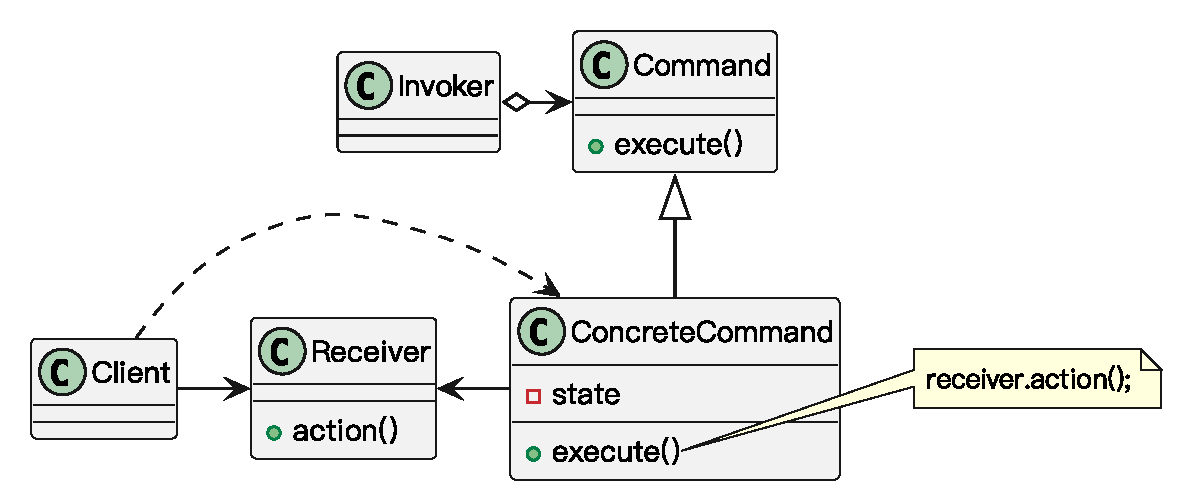
\includegraphics[width=0.65\textwidth]{images/命令模式结构.eps}
    \vspace{-1em}
\end{figure}

\subsubsection{模式分析}
\begin{itemize}
    \item 命令模式的本质是\textbf{对命令进行封装,将发出命令的责任和执行命令的责任分割开}。
    \item 每一个命令都是一个\textbf{操作}:请求的一方发出请求,要求执行一个操作;接收的一方收到请求,并执行操作。
    \item 命令模式允许请求的一方和接收的一方独立开来,使得\textbf{请求的一方不必知道接收请求的一方的接口},更不必知道请求是怎么被接收,以及操作是否被执行、何时被执行,以及是怎么被执行的。
    \item 命令模式\textbf{使请求本身成为一个对象},这个对象和其他对象一样可以被存储和传递。
    \item 命令模式的关键在于\textbf{引入了抽象命令接口},且\textbf{发送者针对抽象命令接口编程},只有实现了抽象命令接口的\textbf{具体命令才能与接收者相关联}。
\end{itemize}

命令模式顺序图
\begin{figure}[H]
    \vspace{-0.5em}
	\centering
	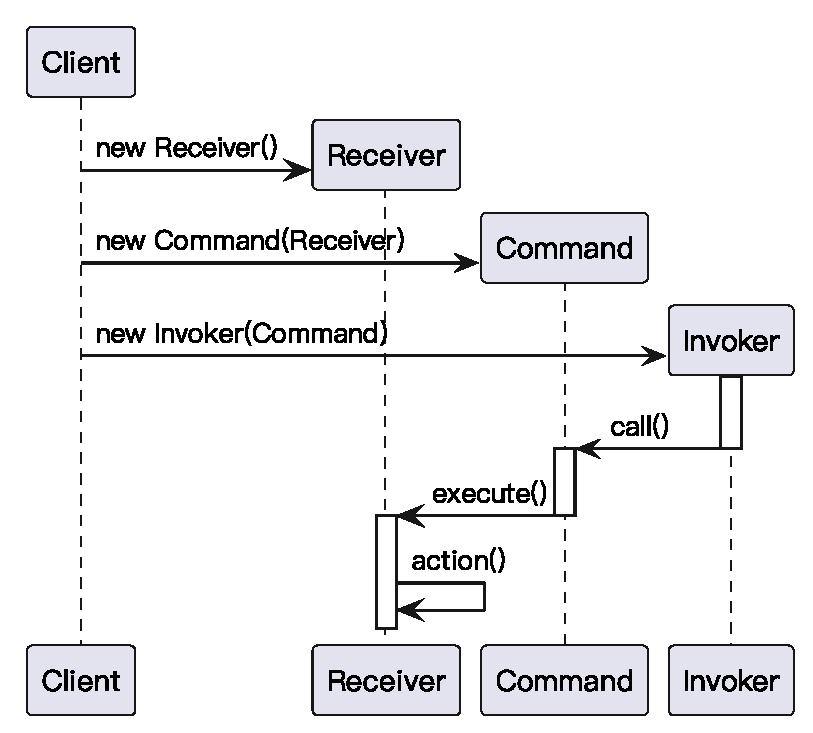
\includegraphics[width=0.5\textwidth]{images/命令模式顺序图.eps}
    \vspace{-1em}
\end{figure}

命令模式典型代码:
\begin{figure}[H]
    \vspace{-0.5em}
	\centering
	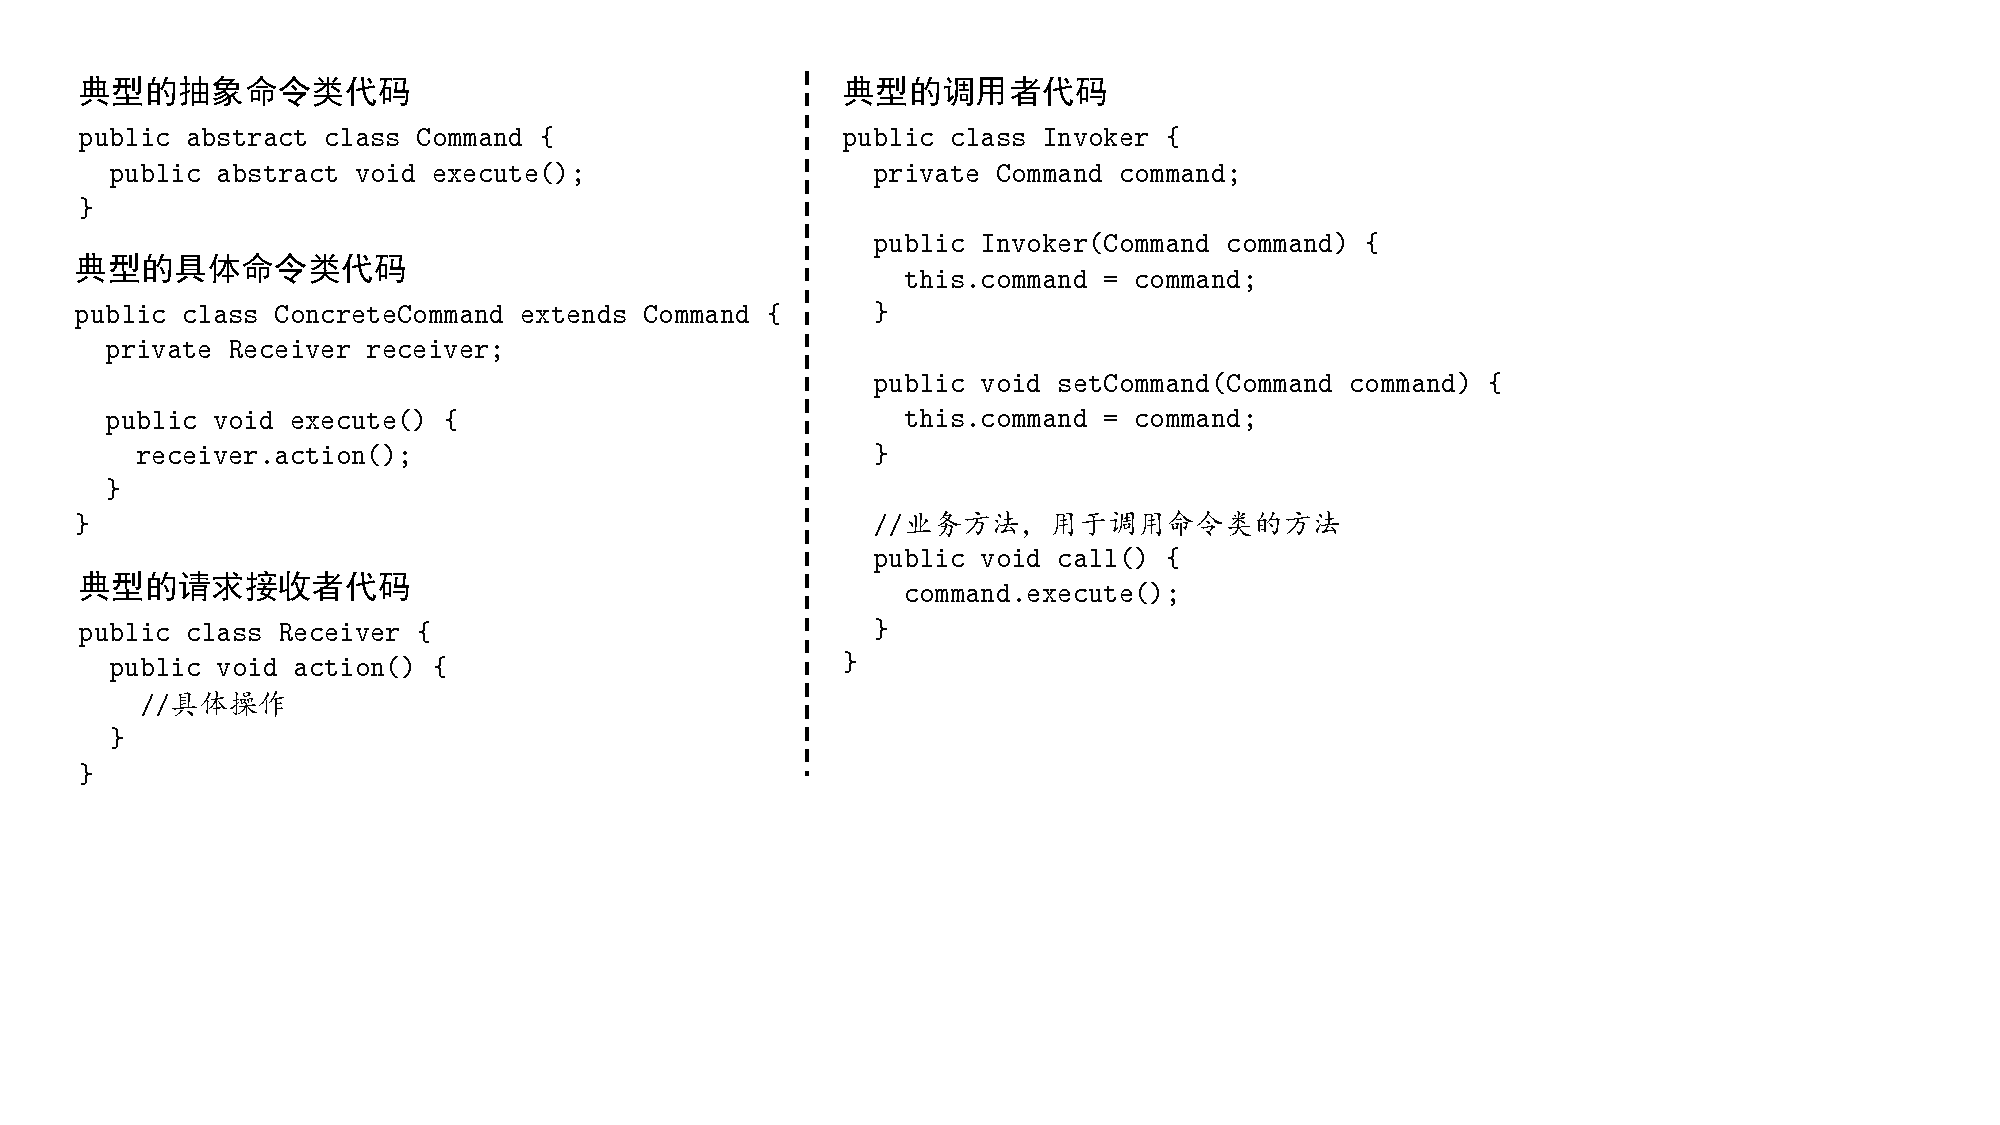
\includegraphics[width=0.75\textwidth]{images/命令模式典型代码.pdf}
    \vspace{-1em}
\end{figure}

\subsubsection{模式实例}
电视机遥控器:电视机是请求的接收者,遥控器是请求的发送者,遥控器上有一些按钮,不同的按钮对应电视机的不同操作。抽象命令角色由一个命令接口来扮演,有三个具体的命令类实现了抽象命令接口,这三个具体命令类分别代表三种操作:打开电视机、关闭电视机和切换频道。显然,电视机遥控器就是一个典型的命令模式应用实例。
\begin{figure}[H]
    \vspace{-0.5em}
	\centering
	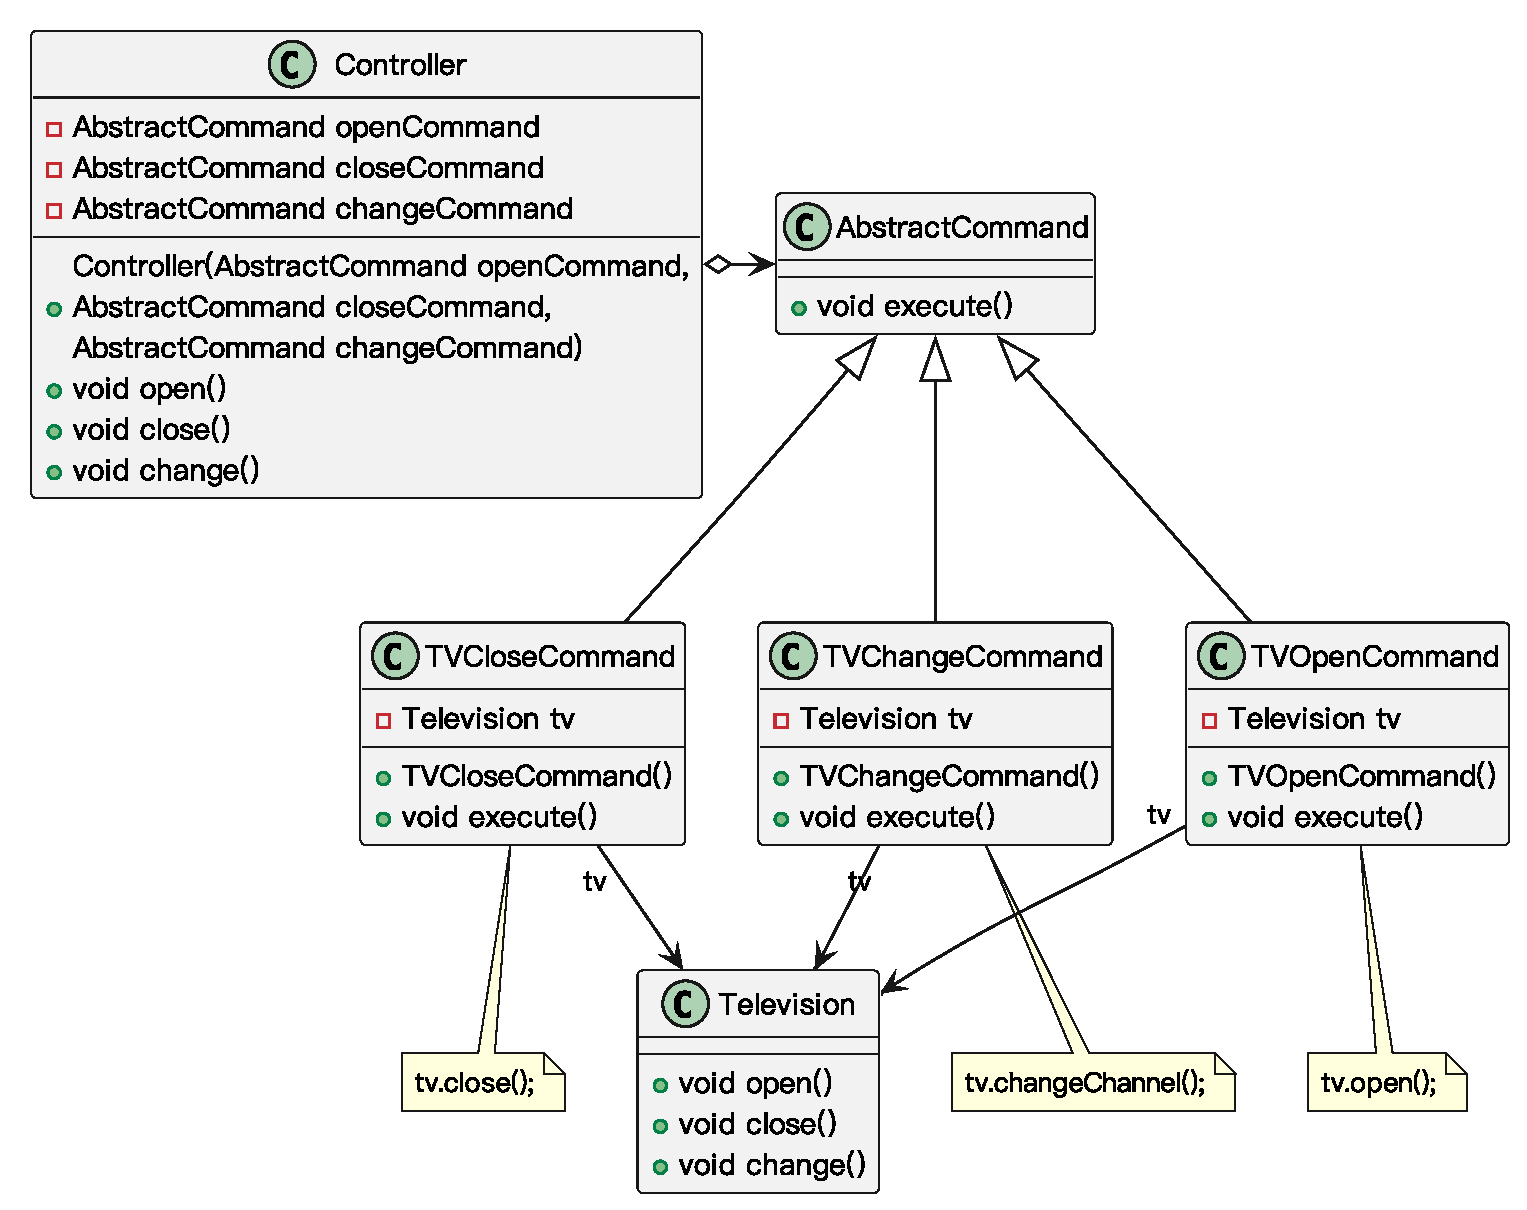
\includegraphics[width=0.85\textwidth]{images/命令模式实例1.eps}
    \vspace{-1em}
\end{figure}

功能键设置:为了用户使用方便,某系统提供了一系列功能键,用户可以自定义功能键的功能,如功能键FunctionButton可以用于退出系统(SystemExitClass),也可以用于打开帮助界面(DisplayHelpClass)。用户可以通过修改配置文件来改变功能键的用途,现使用命令模式来设计该系统,使得功能键类与功能类之间解耦,相同的功能键可以对应不同的功能。
\begin{figure}[H]
    \vspace{-0.5em}
	\centering
	\includegraphics[width=0.85\textwidth]{images/命令模式实例2.eps}
    \vspace{-1em}
\end{figure}

\subsubsection{模式优缺点}
命令模式的优点:
\begin{itemize}
    \item 降低系统的耦合度。
    \item 新的命令可以很容易地加入到系统中。
    \item 可以比较容易地设计一个命令队列和宏命令(组合命令)。
    \item 可以方便地实现对请求的Undo和Redo。
\end{itemize}

命令模式的缺点:
\begin{itemize}
    \item 使用命令模式可能会\textbf{导致某些系统有过多的具体命令类}。因为针对每一个命令都需要设计一个具体命令类,因此某些系统可能需要大量具体命令类,这将影响命令模式的使用。
\end{itemize}

\subsubsection{模式适用环境}
在以下情况下可以使用命令模式:
\begin{itemize}
    \item 系统需要将请求调用者和请求接收者解耦,使得调用者和接收者不直接交互。
    \item 系统需要在不同的时间指定请求、将请求排队和执行请求。
    \item 系统需要支持命令的撤销(Undo)操作和恢复(Redo)操作。
    \item 系统需要将一组操作组合在一起,即支持宏命令。
\end{itemize}

\subsubsection{模式应用}
\ding{172} Java语言使用命令模式实现AWT/Swing GUI的委派事件模型 (Delegation Event Model, DEM) 。
\begin{itemize}
    \item 在AWT/Swing中,Frame、Button等界面组件是请求发送者,而AWT提供的事件监听器接口和事件适配器类是抽象命令接口,用户可以自己写抽象命令接口的子类来实现事件处理,即实现具体命令类,而在具体命令类中可以调用业务处理方法来实现该事件的处理。对于界面组件而言,只需要了解命令接口即可,无须关心接口的实现,组件类并不关心实际操作,而操作由用户来实现。
\end{itemize}

\ding{173} 很多系统都提供了宏命令功能,如Unix平台下的Shell编程,可以将多条命令封装在一个命令对象中,只需要一条简单的命令即可执行一个命令序列,这也是命令模式的应用实例之一。

\vspace{-0.5em}
\begin{shaded}
宏命令又称为组合命令,它是命令模式和组合模式联用的产物。

宏命令也是一个具体命令,不过它包含了对其他命令对象的引用,在调用宏命令的\;\verb|execute()|\;方法时,将递归调用 它所包含的每个成员命令的\;\verb|execute()|\;方法,一个宏命令 的成员对象可以是简单命令,还可以继续是宏命令。执行 一个宏命令将执行多个具体命令,从而实现对命令的批处 理。
\end{shaded}
\vspace{-1em}

\subsubsection{模式扩展}
撤销操作的实现
\begin{figure}[H]
    \vspace{-0.5em}
	\centering
	\includegraphics[width=0.7\textwidth]{images/命令模式拓展1.eps}
    \vspace{-1em}
\end{figure}

宏命令
\begin{figure}[H]
    \vspace{-0.5em}
	\centering
	\includegraphics[width=0.8\textwidth]{images/命令模式拓展2.eps}
    \vspace{-1em}
\end{figure}
	\section{行为型模式}

\subsection{观察者模式}

\subsubsection{模式动机}
建立一种对象与对象之间的依赖关系,\textbf{一个对象发生改变时将自动通知其他对象,其他对象将相应做出反应}。
\begin{itemize}
    \item 发生改变的对象称为观察目标,而被通知的对象称为观察者。
    \item 一个观察目标可以对应多个观察者,而且这些观察者之间没有相互联系,可以根据需要增加和删除观察者,使得系统更易于扩展。
\end{itemize}

\subsubsection{模式定义}
观察者模式(Observer Pattern):定义对象间的一种一对多依赖关系,使得每当一个对象状态发生改变时,其相关依赖对象皆得到通知并被自动更新。观察者模式又叫做发布-订阅(Publish/Subscribe)模式、模型-视图 (Model/View)模式、源-监听器(Source/Listener) 模式或从属者(Dependents)模式。观察者模式是一种对象行为型模式。

\subsubsection{模式结构}
观察者模式包含如下角色:
\vspace{-0.8em}
\begin{multicols}{2}
    \begin{itemize}
        \item Subject:目标
        \item ConcreteSubject:具体目标
        \item Observer:观察者
        \item ConcreteObserver:具体观察者
    \end{itemize}
\end{multicols}
\vspace{-1em}

\begin{figure}[H]
    \vspace{-0.5em}
	\centering
	\includegraphics[width=0.7\textwidth]{images/观察者模式结构.eps}
    \vspace{-1em}
\end{figure}

\subsubsection{模式分析}
\begin{itemize}
    \item 观察者模式描述了\textbf{如何建立对象与对象之间的依赖关系},如何构造满足这种需求的系统。
    \item 这一模式中的关键对象是观察目标和观察者,\textbf{一个目标可以有任意数目的与之相依赖的观察者,一旦目标的状态发生改变,所有的观察者都将得到通知}。
    \item 作为对这个通知的响应,每个观察者都将即时更新自己的状态,以与目标状态同步,这种交互也称为\textbf{发布-订阅}(publish-subscribe)。目标是通知的发布者,它发出通知时并不需要知道谁是它的观察者,可以有任意数目的观察者订阅它并接收通知。
\end{itemize}

观察者模式顺序图如下所示:
\begin{figure}[H]
    \vspace{-0.5em}
	\centering
	\includegraphics[width=0.45\textwidth]{images/观察者模式顺序图.eps}
    \vspace{-1em}
\end{figure}

观察者模式典型代码:
\begin{figure}[H]
    \vspace{-0.5em}
	\centering
	\includegraphics[width=0.95\textwidth]{images/观察者模式典型代码.pdf}
    \vspace{-1em}
\end{figure}

\subsubsection{模式实例}
猫、狗与老鼠:假设猫是老鼠和狗的观察目标,老鼠和狗是观察者,猫叫老鼠跑,狗也跟着叫,使用观察者模式描述该过程。
\begin{figure}[H]
    \vspace{-0.5em}
	\centering
	\includegraphics[width=0.6\textwidth]{images/观察者模式实例1.eps}
    \vspace{-1em}
\end{figure}

自定义登录控件:Java事件处理模型中应用了观察者模式,下面通过一个实例来学习如何自定义Java控件,并给该控件增加相应的事件。该实例基于Java Swing/AWT控件,在Swing/AWT的相关类中封装了对事件的底层处理。
\begin{figure}[H]
    \vspace{-0.5em}
	\centering
	\includegraphics[width=0.85\textwidth]{images/观察者模式实例2.eps}
    \vspace{-1em}
\end{figure}

\subsubsection{模式优缺点}
观察者模式的优点:
\begin{itemize}
    \item 观察者模式可以\textbf{实现表示层和数据逻辑层的分离},并定义了稳定的消息更新传递机制,抽象了更新接口,使得可以有各种各样不同的表示层作为具体观察者角色。
    \item 观察者模式在观察目标和观察者之间\textbf{建立一个抽象的耦合}。
    \item 观察者模式\textbf{支持广播通信}。
    \item 观察者模式\textbf{符合开闭原则}的要求。
\end{itemize}

观察者模式的缺点:
\begin{itemize}
    \item 如果一个观察目标对象有很多直接和间接的观察者的话,\textbf{将所有的观察者都通知到会花费很多时间}。
    \item 如果在观察者和观察目标之间\textbf{有循环依赖}的话,观察目标会触发它们之间进行循环调用,\textbf{可能导致系统崩溃}。
    \item 观察者模式\textbf{没有相应的机制让观察者知道所观察的目标对象是怎么发生变化的},而仅仅只是知道观察目标发生了变化。
\end{itemize}

\subsubsection{模式适用环境}
在以下情况下可以使用观察者模式:
\begin{itemize}
    \item 一个抽象模型有两个方面,其中一个方面依赖于另一个方面。将这些方面封装在独立的对象中使它们可以各自独立地改变和复用。
    \item 一个对象的改变将导致其他一个或多个对象也发生改变,而不知道具体有多少对象将发生改变,可以降低对象之间的耦合度。
    \item 一个对象必须通知其他对象,而并不知道这些对象是谁。需要在系统中创建一个触发链,A对象的行为将影响B对象,B对象的行为将影响C对象……,可以使用观察者模式创建一种链式触发机制。
\end{itemize}

\subsubsection{模式应用}
\ding{172} JDK1.1版本及以后的各个版本中,事件处理模型采用基于观察者模式的委派事件模型(Delegation Event Model, DEM)。
\begin{itemize}
    \item 在DEM中,事件的发布者称为事件源(Event Source),而订阅者叫做事件监听器(Event Listener),在这个过程中还可以通过事件对象(Event Object)来传递与事件相关的信息,可以在事件监听者的实现类中实现事件处理,因此事件监听对象又可以称为事件处理对象。
    \item 事件源对象、事件监听对象(事件处理对象)和事件对象构成了Java事件处理模型的三要素。
\end{itemize}

\ding{173} 除了AWT中的事件处理之外,Java语言解析XML的技术SAX2以及Servlet技术的事件处理机制都基于DEM,它们都是观察者模式的应用。

\ding{174} 观察者模式在软件开发中应用非常广泛,如某电子商务网站可以在执行发送操作后给用户多个发送商品打折信息,某团队战斗游戏中某队友牺牲将给所有成员提示等等,\textbf{凡是涉及到一对一或者一对多的对象交互场景都可以使用观察者模式}。

\subsubsection{模式扩展}
\paragraph*{Java语言提供的对观察者模式的支持}~{} \par
在JDK的\sverb|java.util|\;包中,提供了\sverb|Observable|\;类以及\sverb|Observer|\;接口,它们构成了Java语言对观察者模式的支持。
\begin{figure}[H]
    \vspace{-0.5em}
	\centering
	\includegraphics[width=0.68\textwidth]{images/观察者模式拓展1.eps}
    \vspace{-1em}
\end{figure}

\paragraph*{MVC模式}~{} \par
MVC模式是一种架构模式,它包含三个角色:模型(Model),视图(View)和控制器(Controller)。观察者模式可以用来实现MVC模式,观察者模式中的观察目标就是MVC模式中的模型(Model),而观察者就是MVC中的视图(View),控制器(Controller)充当两者之间的中介者(Mediator)。当模型层的数据发生改变时,视图层将自动改变其显示内容。
\begin{figure}[H]
    \vspace{-0.5em}
	\centering
	\includegraphics[width=0.45\textwidth]{images/观察者模式拓展2.pdf}
    \vspace{-1em}
\end{figure}


\subsection{中介者模式}

\subsubsection{模式动机}
在用户与用户直接聊天的设计方案中,用户对象之间存在很强的关联性,将导致系统出现如下问题:
\begin{itemize}
    \item \textbf{系统结构复杂}:对象之间存在大量的相互关联和调用,若有一个对象发生变化,则需要跟踪和该对象关联的其他所有对象,并进行适当处理。
    \item \textbf{对象可重用性差}:由于一个对象和其他对象具有很强的关联,若没有其他对象的支持,一个对象很难被另一个系统或模块重用,这些对象表现出来更像一个不可分割的整体,职责较为混乱。
    \item \textbf{系统扩展性低}:增加一个新的对象需要在原有相关对象上增加引用,增加新的引用关系也需要调整原有对象,系统耦合度很高,对象操作很不灵活,扩展性差。
\end{itemize}

在面向对象的软件设计与开发过程中,根据“单一职责原则”,我们应该尽量将对象细化,使其只负责或呈现单一的职责。

对于一个模块,可能由很多对象构成,而且这些对象之间可能存在相互的引用,\textbf{为了减少对象两两之间复杂的引用关系,使之成为一个松耦合的系统,我们需要使用中介者模式},这就是中介者模式的模式动机。

\subsubsection{模式定义}
中介者模式(Mediator Pattern)定义:用一个中介对象来封装一系列的对象交互,中介者使各对象不需要显式地相互引用,从而使其耦合松散,而且可以独立地改变它们之间的交互。中介者模式又称为调停者模式,它是一种对象行为型模式。

\subsubsection{模式结构}
中介者模式包含如下角色:
\vspace{-0.8em}
\begin{multicols}{2}
    \begin{itemize}
        \item Mediator:抽象中介者
        \item ConcreteMediator:具体中介者
        \item Colleague:抽象同事类
        \item ConcreteColleague:具体同事类
    \end{itemize}
\end{multicols}
\vspace{-1em}

\begin{figure}[H]
    \vspace{-0.5em}
	\centering
	\includegraphics[width=0.7\textwidth]{images/中介者模式结构.eps}
    \vspace{-1em}
\end{figure}

\subsubsection{模式分析}
中介者模式可以使对象之间的关系数量急剧减少:
\begin{figure}[H]
    \vspace{-0.5em}
	\centering
	\includegraphics[width=0.68\textwidth]{images/中介者模式分析.pdf}
    \vspace{-1em}
\end{figure}

中介者承担两方面的职责:
\begin{itemize}
    \item \textbf{中转作用(结构性)}:通过中介者提供的中转作用,各个同事对象就不再需要显式引用其他同事,当需要和其他同事进行通信时,通过中介者即可。该中转作用属于中介者\textbf{在结构上的支持}。
    \item \textbf{协调作用(行为性)}:中介者可以更进一步的对同事之间的关系进行封装,同事可以一致地和中介者进行交互,而不需要指明中介者需要具体怎么做,中介者根据封装在自身内部的协调逻辑,对同事的请求进行进一步处理,将同事成员之间的关系行为进行分离和封装。该协调作用属于中介者\textbf{在行为上的支持}。
\end{itemize}

中介者模式典型代码:
\begin{figure}[H]
    \vspace{-0.5em}
	\centering
	\includegraphics[width=\textwidth]{images/中介者模式典型代码.pdf}
    \vspace{-2em}
\end{figure}

\subsubsection{模式实例}
虚拟聊天室:某论坛系统欲增加一个虚拟聊天室,允许论坛会员通过该聊天室进行信息交流,普通会员(CommonMember)可以给其他会员发送文本信息,钻石会员(DiamondMember)既可以给其他会员发送文本信息,还可以发送图片信息。该聊天室可以对不雅字符进行过滤,如“日”等字符;还可以对发送的图片大小进行控制。用中介者模式设计该虚拟聊天室。
\begin{figure}[H]
    \vspace{-0.5em}
	\centering
	\includegraphics[width=0.95\textwidth]{images/中介者模式实例.eps}
    \vspace{-1em}
\end{figure}

\subsubsection{模式优缺点}
中介者模式的优点:
\vspace{-0.8em}
\begin{multicols}{2}
    \begin{itemize}
        \item 简化了对象之间的交互。
        \item 将各同事解耦。
        \item 减少子类生成。
        \item 可以简化各同事类的设计和实现。
    \end{itemize}
\end{multicols}
\vspace{-1em}

中介者模式的缺点:
\begin{itemize}
    \item 在具体中介者类中包含了同事之间的交互细节,可能会导致具体中介者类非常复杂,使得系统难以维护。
\end{itemize}

\subsubsection{模式适用环境}
在以下情况下可以使用中介者模式:
\begin{itemize}
    \item 系统中\textbf{对象之间存在复杂的引用关系},产生的相互依赖关系结构混乱且难以理解。
    \item 一个对象由于引用了其他很多对象并且直接和这些对象通信,导致\textbf{难以复用该对象}。
    \item \textbf{想通过一个中间类来封装多个类中的行为,而又不想生成太多的子类}。可以通过引入中介者类来实现,在中介者中定义对象交互的公共行为,如果需要改变行为则可以增加新的中介者类。
\end{itemize}

\subsubsection{模式应用}
\ding{172} 中介者模式在事件驱动类软件中应用比较多,在设计GUI应用程序时,组件之间可能存在较为复杂的交互关系,一个组件的改变将影响与之相关的其他组件,此时可以使用中介者模式来对组件进行协调。

\ding{173} MVC是Java EE的一个基本模式,此时控制器Controller作为一种中介者,它负责控制视图对象View和模型对象Model之间的交互。如在Struts中,Action就可以作为JSP页面与业务对象之间的中介者。

\subsubsection{模式扩展}
\paragraph*{中介者模式与迪米特法则}~{} \par
在中介者模式中,通过创造出一个中介者对象,\textbf{将系统中有关的对象所引用的其他对象数目减少到最少},使得一个对象与其同事之间的相互作用被这个对象与中介者对象之间的相互作用所取代。因此,\textbf{中介者模式就是迪米特法则的一个典型应用}。

\paragraph*{中介者模式与GUI开发}~{} \par
中介者模式可以方便地应用于图形界面(GUI)开发中,在比较复杂的界面中可能存在多个界面组件之间的交互关系。

对于这些复杂的交互关系,有时候我们可以引入一个中介者类,\textbf{将这些交互的组件作为具体的同事类,将它们之间的引用和控制关系交由中介者负责},在一定程度上简化系统的交互,这也是中介者模式的常见应用之一。


\subsection{模板方法模式}

\subsubsection{模式动机}
模板方法模式是\textbf{基于继承}的代码复用基本技术,模板方法模式的结构和用法也是面向对象设计的核心之一。在模板方法模式中,可以\textbf{将相同的代码放在父类中,而将不同的方法实现放在不同的子类中}。

在模板方法模式中,我们需要准备一个抽象类,将部分逻辑以具体方法以及具体构造函数的形式实现,然后声明一些抽象方法来让子类实现剩余的逻辑。不同的子类可以以不同的方式实现这些抽象方法,从而对剩余的逻辑有不同的实现,这就是模板方法模式的用意。模板方法模式体现了面向对象的诸多重要思想,是一种使用频率较高的模式。

\subsubsection{模式定义}
模板方法模式(Template Method Pattern):定义一个操作中算法的骨架,而将一些步骤延迟到子类中,模板方法使得子类可以不改变一个算法的结构即可重定义该算法的某些特定步骤。模板方法是一种类行为型模式。

\subsubsection{模式结构}
模板方法模式包含如下角色:
\vspace{-0.8em}
\begin{multicols}{2}
    \begin{itemize}
        \item AbstractClass:抽象类
        \item ConcreteClass:具体子类
    \end{itemize}
\end{multicols}
\vspace{-1em}

\begin{figure}[H]
    \vspace{-0.5em}
	\centering
	\includegraphics[width=0.45\textwidth]{images/模板方法模式结构.eps}
    \vspace{-1em}
\end{figure}

\subsubsection{模式分析}
模板方法模式是一种类的行为型模式,在它的结构图中\textbf{只有类之间的继承关系,没有对象关联关系}。

在模板方法模式的使用过程中,要求开发抽象类和开发具体子类的设计师之间进行协作。一个设计师负责\textbf{给出一个算法的轮廓和骨架},另一些设计师则负责\textbf{给出这个算法的各个逻辑步骤}。实现这些具体逻辑步骤的方法称为\textbf{基本方法}(Primitive Method),而将这些基本法方法汇总起来的方法称为\textbf{模板方法}(Template Method),模板方法模式的名字从此而来。
\begin{itemize}
    \item 模板方法:一个模板方法是定义在抽象类中的、把基本操作方法组合在一起形成一个总算法或一个总行为的方法。
    \item 基本方法:基本方法是实现算法各个步骤的方法,是模板方法的组成部分。
    \vspace{-0.8em}
    \begin{multicols}{3}
    \begin{itemize}
        \item 抽象方法
        \item 具体方法
        \item 钩子方法
    \end{itemize}
    \end{multicols}
    \vspace{-1em}
\end{itemize}
钩子方法(Hook Method):
\begin{lstlisting}
public void template(){
    open();
    display();
    if(isPrint()){
        print();
    }
}
public boolean isPrint(){
    return true;
}
\end{lstlisting}

模板方法模式典型代码:
\begin{figure}[H]
	\centering
	\includegraphics[width=\textwidth]{images/模板方法模式分析.pdf}
    \vspace{-2em}
\end{figure}

在模板方法模式中,由于面向对象的多态性,子类对象在运行时将覆盖父类对象,子类中定义的方法也将覆盖父类中定义的方法,因此程序在运行时,\textbf{具体子类的基本方法将覆盖父类中定义的基本方法,子类的钩子方法也将覆盖父类的钩子方法},从而可以通过在子类中实现的钩子方法对父类方法的执行进行约束,实现子类对父类行为的反向控制。

\subsubsection{模式实例}
银行业务办理流程:在银行办理业务时,一般都包含几个基本步骤,首先需要取号排队,然后办理具体业务,最后需要对银行工作人员进行评分。无论具体业务是取款、存款还是转账,其基本流程都一样。现使用模板方法模式模拟银行业务办理流程。
\begin{figure}[H]
    \vspace{-0.5em}
	\centering
	\includegraphics[width=0.55\textwidth]{images/模板方法模式实例1.eps}
    \vspace{-1em}
\end{figure}


数据库操作模板:对数据库的操作一般包括连接、打开、使用、关闭等步骤,在数据库操作模板类中我们定义了\sverb|connDB()|、\sverb|openDB()|、\sverb|useDB()|、\sverb|closeDB()|\;四个方法分别对应这四个步骤。对于不同类型的数据库(如SQL Server和Oracle),其操作步骤都一致,只是连接数据库\sverb|connDB()|\;方法有所区别,现使用模板方法模式对其进行设计。
\begin{figure}[H]
    \vspace{-0.5em}
	\centering
	\includegraphics[width=0.5\textwidth]{images/模板方法模式实例2.eps}
    \vspace{-1em}
\end{figure}

\subsubsection{模式优缺点}
模板方法模式的优点:
\begin{itemize}
    \item 模板方法模式在一个类中抽象地定义算法,而由它的子类实现细节的处理。
    \item 模板方法模式是一种代码复用的基本技术。
    \item 模板方法模式导致一种反向的控制结构,通过一个父类调用其子类的操作,通过对子类的扩展增加新的行为,符合“开闭原则”。
\end{itemize}

模板方法模式的缺点:
\begin{itemize}
    \item 每个不同的实现都需要定义一个子类,这会导致类的个数增加,系统更加庞大,设计也更加抽象,但是更加符合“单一职责原则”,使得类的内聚性得以提高。
\end{itemize}

\subsubsection{模式适用环境}
在以下情况下可以使用模板方法模式:
\begin{itemize}
    \item 一次性实现一个算法的不变的部分,并将可变的行为留给子类来实现。
    \item 各子类中公共的行为应被提取出来并集中到一个公共父类中以避免代码重复。
    \item 对一些复杂的算法进行分割,将其算法中固定不变的部分设计为模板方法和父类具体方法,而一些可以改变的细节由其子类来实现。
    \item 控制子类的扩展。
\end{itemize}

\subsubsection{模式应用}
\ding{172} 模板方法模式广泛应用于框架设计(如Spring,Struts等)中,以确保父类控制处理流程的逻辑顺序(如框架的初始化)。

\ding{173} Java单元测试工具JUnit中的\sverb|TestCase|\;类的设计:
\begin{lstlisting}
...
public void runBare() throws Throwable {
    setUp();
    try {
        runTest(); 
    }finally { 
        tearDown();
    }
}
...
\end{lstlisting}

\subsubsection{模式扩展}

\paragraph*{关于继承的讨论}~{} \par
模板方法模式鼓励我们\textbf{恰当使用继承},此模式可以用来改写一些拥有相同功能的相关类,\textbf{将可复用的一般性的行为代码移到父类里面},而将特殊化的行为代码移到子类里面。这也进一步说明,虽然继承复用存在一些问题,但是在某些情况下还是可以给开发人员带来方便,\textbf{模板方法模式就是体现继承优势的模式之一}。

\paragraph*{好莱坞原则}~{} \par
在模板方法模式中,子类不显式调用父类的方法,而是通过覆盖父类的方法来实现某些具体的业务逻辑,父类控制对子类的调用,这种机制被称为好莱坞原则(Hollywood Principle),好莱坞原则的定义为:“不要给我们打电话,我们会给你打电话”。

在模板方法模式中,好莱坞原则体现在:\textbf{子类不需要调用父类,而通过父类来调用子类},将某些步骤的实现写在子类中,由父类来控制整个过程。

\paragraph*{钩子方法的使用}~{} \par
\begin{itemize}
    \item 钩子方法的引入使得子类可以控制父类的行为。
    \item 最简单的钩子方法就是空方法,也可以在钩子方法中定义一个默认的实现,如果子类不覆盖钩子方法,则执行父类的默认实现代码。
    \item 比较复杂一点的钩子方法可以对其他方法进行约束,这种钩子方法通常返回一个\sverb|boolean|\;类型,即返回\sverb|true|\;或\sverb|false|,用来判断是否执行某一个基本方法。
\end{itemize}


	\section{适配器与组合}

\subsection{适配器模式}

\subsubsection{模式动机}
在软件开发中采用类似于电源适配器的设计和编码技巧被称为适配器模式。
\begin{itemize}
    \item 通常情况下,客户端可以通过目标类的接口访问它所提供的服务。有时,现有的类可以满足客户类的功能需要,但是它所提供的接口不一定是客户类所期望的,这可能是因为现有类中方法名与目标类中定义的方法名不一致等原因所导致的。
    \item 在这种情况下,现有的接口需要转化为客户类期望的接口,这样保证了对现有类的重用。如果不进行这样的转化,客户类就不能利用现有类所提供的功能,适配器模式可以完成这样的转化。
\end{itemize}

在适配器模式中可以定义一个包装类,包装不兼容接口的对象,这个包装类指的就是\textbf{适配器}(Adapter),它所包装的对象就是\textbf{适配者}(Adaptee),即被适配的类。

适配器提供客户类需要的接口,\textbf{适配器的实现就是把客户类的请求转化为对适配者的相应接口的调用}。也就是说:当客户类调用适配器的方法时,在适配器类的内部将调用适配者类的方法,而这个过程对客户类是透明的,客户类并不直接访问适配者类。因此,\textbf{适配器可以使由于接口不兼容而不能交互的类可以一起工作}。这就是适配器模式的模式动机。

\subsubsection{模式定义}
适配器模式(Adapter Pattern):将一个接口转换成客户希望的另一个接口,适配器模式使接口不兼容的那些类可以一起工作,其别名为包装器(Wrapper)。适配器模式既可以作为类结构型模式,也可以作为对象结构型模式。

\subsubsection{模式结构}
适配器模式包含如下角色:
\vspace{-0.8em}
\begin{multicols}{2}
    \begin{itemize}
        \item Target:目标抽象类
        \item Adapter:适配器类
        \item Adaptee:适配者类
        \item Client:客户类
    \end{itemize}
\end{multicols}
\vspace{-1em}

\begin{figure}[H]
	\centering
    \vspace{-0.5em}
	\subfloat[对象适配器模式结构]{
	\begin{minipage}[t]{0.48\linewidth}
		\centering
		\includegraphics[width=0.97\linewidth]{images/对象适配器模式结构.eps}
	\end{minipage}
	}
    \subfloat[类适配器模式结构]{
    \begin{minipage}[t]{0.48\linewidth}
        \centering
        \includegraphics[width=0.97\linewidth]{images/类适配器模式结构.eps}
    \end{minipage}
    }
	\centering
    \vspace{-1em}
\end{figure}

\subsubsection{模式分析}
适配器模式典型代码如下:
\begin{figure}[H]
    \vspace{-0.5em}
	\centering
	\includegraphics[width=0.9\textwidth]{images/适配器模式分析.pdf}
    \vspace{-1em}
\end{figure}

\subsubsection{模式实例}
仿生机器人:现需要设计一个可以模拟各种动物行为的机器人,在机器人中定义了一系列方法,如机器人叫喊方法\sverb|cry()|、机器人移动方法\sverb|move()|\;等。如果希望在不修改已有代码的基础上使得机器人能够像狗一样叫,像狗一样跑,使用适配器模式进行系统设计。
\begin{figure}[H]
    \vspace{-0.5em}
	\centering
	\includegraphics[width=0.3\textwidth]{images/适配器模式实例1.eps}
    \vspace{-1em}
\end{figure}

加密适配器:某系统需要提供一个加密模块,将用户信息(如密码等机密信息)加密之后再存储在数据库中,系统已经定义好了数据库操作类。为了提高开发效率,现需要重用已有的加密算法,这些算法封装在一些由第三方提供的类中,有些甚至没有源代码。使用适配器模式设计该加密模块,实现在不修改现有类的基础上重用第三方加密方法。
\begin{figure}[H]
    \vspace{-0.5em}
	\centering
	\includegraphics[width=0.75\textwidth]{images/适配器模式实例2.eps}
    \vspace{-1em}
\end{figure}

\subsubsection{模式优缺点}
适配器模式的优点:
\begin{itemize}
    \item \textbf{将目标类和适配者类解耦},通过引入一个适配器类来重用现有的适配者类,而无须修改原有代码。
    \item \textbf{增加了类的透明性和复用性},将具体的实现封装在适配者类中,对于客户端类来说是透明的,而且提高了适配者的复用性。
    \item \textbf{灵活性和扩展性都非常好},通过使用配置文件,可以很方便地更换适配器,也可以在不修改原有代码的基础上增加新的适配器类,完全符合“开闭原则”。
\end{itemize}

类适配器模式还具有如下优点:
\begin{itemize}
    \item 由于适配器类是适配者类的子类,因此\textbf{可以在适配器类中置换一些适配者的方法},使得适配器的灵活性更强。
\end{itemize}

对象适配器模式还具有如下优点:
\begin{itemize}
    \item 一个对象适配器可以把多个不同的适配者适配到同一个目标,也就是说,\textbf{同一个适配器可以把适配者类和它的子类都适配到目标接口}。
\end{itemize}

类适配器模式的缺点如下:
\begin{itemize}
    \item 对于Java、C\#等不支持多重继承的语言,一次最多只能适配一个适配者类,而且目标抽象类只能为抽象类,不能为具体类,\textbf{其使用有一定的局限性},不能将一个适配者类和它的子类都适配到目标接口。
\end{itemize}

对象适配器模式的缺点如下:
\begin{itemize}
    \item 与类适配器模式相比,\textbf{要想置换适配者类的方法就不容易}。如果一定要置换掉适配者类的一个或多个方法,就只好先做一个适配者类的子类,将适配者类的方法置换掉,然后再把适配者类的子类当做真正的适配者进行适配,实现过程较为复杂。
\end{itemize}

\subsubsection{模式适用环境}
在以下情况下可以使用适配器模式:
\begin{itemize}
    \item 系统需要使用现有的类,而这些类的接口不符合系统的需要。
    \item 想要建立一个可以重复使用的类,用于与一些彼此之间没有太大关联的一些类,包括一些可能在将来引进的类一起工作。
\end{itemize}

\subsubsection{模式应用}
\ding{172} Sun公司在1996年公开了Java语言的数据库连接工具JDBC,JDBC使得Java语言程序能够与数据库连接,并使用SQL语言来查询和操作数据。JDBC给出一个客户端通用的抽象接口,每一个具体数据库引擎(如SQL Server、Oracle、MySQL等)的JDBC驱动软件都是一个介于JDBC接口和数据库引擎接口之间的适配器软件。抽象的JDBC接口和各个数据库引擎API之间都需要相应的适配器软件,这就是为各个不同数据库引擎准备的驱动程序。

\ding{173} 在JDK类库中也定义了一系列适配器类,如在\sverb|com.sun.imageio.plugins.common|\; 包中定义的\sverb|Input| \verb|StreamAdapter|\;类,用于包装\sverb|ImageInputStream|\;接口及其子类对象。
\begin{lstlisting}
public class InputStreamAdapter extends InputStream{
    ImageInputStream stream;
    public InputStreamAdapter(ImageInputStream stream) {
        super();
        this.stream = stream;
    }
    public int read() throws IOException {
        return stream.read();
    }
    public int read(byte b[], int off, int len) throws IOException {
        return stream.read(b, off, len);
    }
}
\end{lstlisting}

\subsubsection{模式扩展}

\paragraph*{默认适配器模式(缺省适配器模式)}~{} \par
当不需要全部实现接口提供的方法时,可先设计一个抽象类实现接口,并为该接口中每个方法提供一个默认实现(空方法),那么该抽象类的子类可有选择地覆盖父类的某些方法来实现需求,它适用于一个接口不想使用其所有的方法的情况。因此也称为单接口适配器模式。
\begin{figure}[H]
	\centering
    \vspace{-0.5em}
	\subfloat{
	\begin{minipage}[c]{0.48\linewidth}
		\centering
		\includegraphics[width=0.97\linewidth]{images/适配器模式拓展1.eps}
	\end{minipage}
	}
    \hfill
    \subfloat{
    \begin{minipage}[c]{0.4\linewidth}
        \centering
        \includegraphics[width=0.97\linewidth]{images/适配器模式拓展2.eps}
    \end{minipage}
    }
	\centering
    \vspace{-1em}
\end{figure}

\paragraph*{双向适配器}~{} \par
在对象适配器的使用过程中,如果在适配器中同时包含对目标类和适配者类的引用,适配者可以通过它调用目标类中的方法,目标类也可以通过它调用适配者类中的方法,那么该适配器就是一个双向适配器。
\begin{figure}[H]
    \vspace{-0.5em}
	\centering
	\includegraphics[width=\textwidth]{images/适配器模式拓展3.eps}
    \vspace{-1em}
\end{figure}


\subsection{组合模式}
对于\textbf{树形结构},当容器对象(如文件夹)的某一个方法被调用时,将遍历整个树形结构,寻找也包含这个方法的成员对象(可以是容器对象,也可以是叶子对象,如子文件夹和文件)并调用执行。\textbf{(递归调用)}

由于容器对象和叶子对象在功能上的区别,在使用这些对象的客户端代码中必须有区别地对待容器对象和叶子对象,而\textbf{实际上大多数情况下客户端希望一致地处理它们,因为对于这些对象的区别对待将会使得程序非常复杂}。

组合模式描述了如何将容器对象和叶子对象进行递归组合,使得用户在使用时无须对它们进行区分,可以一致地对待容器对象和叶子对象,这就是组合模式的模式动机。

\subsubsection{模式定义}
组合模式(Composite Pattern):组合多个对象形成树形结构以表示“整体-部分”的结构层次。组合模式对单个对象(即叶子对象)和组合对象(即容器对象)的使用具有一致性。

组合模式又可以称为整体-部分(Part-Whole)模式,属于对象的结构模式,它将对象组织到树结构中,可以用来描述整体与部分的关系。

\subsubsection{模式结构}
组合模式包含如下角色:
\vspace{-0.8em}
\begin{multicols}{2}
    \begin{itemize} 
        \item Component:抽象构件
        \item Leaf:叶子构件
        \item Composite:容器构件
        \item Client:客户类
    \end{itemize}
\end{multicols}
\vspace{-1em}

\begin{figure}[H]
    \vspace{-0.5em}
	\centering
	\includegraphics[width=0.6\textwidth]{images/组合模式结构.eps}
    \vspace{-1em}
\end{figure}

\subsubsection{模式分析}
组合模式的关键是\textbf{定义了一个抽象构件类},它既可以代表叶子,又可以代表容器,而\textbf{客户端针对该抽象构件类进行编程},无须知道它到底表示的是叶子还是容器,可以对其进行统一处理。

同时\textbf{容器对象与抽象构件类之间还建立一个聚合关联关系},在容器对象中既可以包含叶子,也可以包含容器,以此实现\textbf{递归}组合,形成一个\textbf{树形结构}。

文件系统组合模式结构图:
\begin{figure}[H]
	\centering
    \vspace{-0.5em}
	\subfloat{
	\begin{minipage}[c]{0.6\linewidth}
		\centering
		\includegraphics[width=0.95\linewidth]{images/组合模式分析.eps}
	\end{minipage}
	}
    \subfloat{
    \begin{minipage}[c]{0.35\linewidth}
        \centering
        \includegraphics[width=0.4\linewidth]{images/文件系统目录.png}
    \end{minipage}
    }
	\centering
    \vspace{-1em}
\end{figure}

组合模式典型代码:
\begin{figure}[H]
    \vspace{-0.5em}
	\centering
	\includegraphics[width=0.85\textwidth]{images/组合模式典型代码.pdf}
    \vspace{-1em}
\end{figure}

\subsubsection{模式实例}
水果盘:在水果盘(Plate)中有一些水果,如苹果(Apple)、香蕉(Banana)、梨子(Pear),当然大水果盘中还可以有小水果盘,现需要对盘中的水果进行遍历(吃),当然如果对一个水果盘执行“吃”方法,实际上就是吃其中的水果。使用组合模式模拟该场景。
\begin{figure}[H]
    \vspace{-0.5em}
	\centering
	\includegraphics[width=0.72\textwidth]{images/组合模式实例1.eps}
    \vspace{-1em}
\end{figure}

文件浏览:文件有不同类型,不同类型的文件其浏览方式有所区别,如文本文件和图片文件的浏览方式就不相同。对文件夹的浏览实际上就是对其中所包含文件的浏览,而客户端可以一致地对文件和文件夹进行操作,无须关心它们的区别。使用组合模式来模拟文件的浏览操作。
\begin{figure}[H]
    \vspace{-0.5em}
	\centering
	\includegraphics[width=\textwidth]{images/组合模式实例2.eps}
    \vspace{-1em}
\end{figure}

\subsubsection{模式优缺点}
组合模式的优点:
\begin{itemize}
    \item 可以清楚地定义\textbf{分层次的复杂对象},表示对象的全部或部分层次,使得增加新构件也更容易。
    \item 客户端调用简单,\textbf{客户端可以一致的使用组合结构或其中单个对象}。
    \item 定义了包含叶子对象和容器对象的\textbf{类层次结构},叶子对象可以被组合成更复杂的容器对象,而这个容器对象又可以被组合,这样不断递归下去,\textbf{可以形成复杂的树形结构}。
    \item \textbf{更容易在组合体内加入对象构件},客户端不必因为加入了新的对象构件而更改原有代码。组合模式
\end{itemize}

组合模式的缺点:
\begin{itemize}
    \item \textbf{使设计变得更加抽象},对象的业务规则如果很复杂,则实现组合模式具有很大挑战性,而且不是所有的方法都与叶子对象子类都有关联。
    \item 增加新构件时可能会产生一些问题,\textbf{很难对容器中的构件类型进行限制}。
\end{itemize}

\subsubsection{模式适用环境}
在以下情况下可以使用组合模式:
\begin{itemize}
    \item 需要表示一个\textbf{对象整体或部分层次},在具有整体和部分的层次结构中,希望通过一种方式忽略整体与部分的差异,可以一致地对待它们。
    \item 让客户能够忽略不同对象层次的变化,客户端可以\textbf{针对抽象构件编程},无须关心对象层次结构的细节。
    \item 对象的结构是动态的并且复杂程度不一样,但客户需要\textbf{一致地处理它们}。
\end{itemize}

\subsubsection{模式应用}
\ding{172} XML文档解析
\begin{figure}[H]
	\centering
    \vspace{-0.5em}
	\subfloat{
	\begin{minipage}[c]{0.58\linewidth}
		\centering
		\includegraphics[width=0.97\linewidth]{images/组合模式应用1.pdf}
	\end{minipage}
	}
    \subfloat{
    \begin{minipage}[c]{0.38\linewidth}
        \centering
        \includegraphics[width=0.97\linewidth]{images/组合模式应用2.pdf}
    \end{minipage}
    }
	\centering
    \vspace{-1em}
\end{figure}

\ding{173} 操作系统中的目录结构是一个树形结构,因此在对文件和文件夹进行操作时可以应用组合模式,例如杀毒软件在查毒或杀毒时,既可以针对一个具体文件,也可以针对一个目录。如果是对目录查毒或杀毒,将递归处理目录中的每一个子目录和文件。

\ding{174} JDK的AWT/Swing是组合模式在Java类库中的一个典型实际应用。
\begin{figure}[H]
    \vspace{-0.5em}
	\centering
	\includegraphics[width=0.65\textwidth]{images/组合模式应用3.eps}
    \vspace{-1em}
\end{figure}

\subsubsection{模式扩展}
更复杂的组合模式
\begin{figure}[H]
    \vspace{-0.5em}
	\centering
	\includegraphics[width=0.57\textwidth]{images/更复杂的组合模式.eps}
    \vspace{-1em}
\end{figure}

透明组合模式
\begin{figure}[H]
    \vspace{-0.5em}
	\centering
	\includegraphics[width=0.45\textwidth]{images/透明组合模式.eps}
    \vspace{-1em}
\end{figure}

安全组合模式
\begin{figure}[H]
    \vspace{-0.5em}
	\centering
	\includegraphics[width=0.43\textwidth]{images/安全组合模式.eps}
    \vspace{-1em}
\end{figure}


	\section{桥接与装饰者}

\subsection{桥接模式}

\subsubsection{模式动机}
设想如果要绘制矩形、圆形、椭圆、正方形,我们至少需要4个形状类,但是如果绘制的图形需要具有不同的颜色,如红色、绿色、蓝色等,此时至少有如下两种设计方案:
\begin{figure}[H]
    \vspace{-0.5em}
	\centering
	\includegraphics[width=0.95\textwidth]{images/桥接模式动机.pdf}
    \vspace{-1em}
\end{figure}
\begin{itemize}
    \item 第一种设计方案是为每一种形状都提供一套各种颜色的版本。
    \item 第二种设计方案是根据实际需要对形状和颜色进行组合。
\end{itemize}

对于有两个变化维度(即两个变化的原因)的系统,采用方案二来进行设计系统中类的个数更少,且系统扩展更为方便。设计方案二即是桥接模式的应用。桥接模式\textbf{将继承关系转换为关联关系,从而降低了类与类之间的耦合,减少了代码编写量}。

\subsubsection{模式定义}
桥接模式(Bridge Pattern):将抽象部分与它的实现部分分离,使它们都可以独立地变化。它是一种对象结构型模式,又称为柄体(Handle and Body)模式或接口(Interface)模式。

\subsubsection{模式结构}
桥接模式包含如下角色:
\vspace{-0.8em}
\begin{multicols}{2}
    \begin{itemize}
        \item Abstraction:抽象类
        \item RefinedAbstraction:扩充抽象类
        \item Implementor:实现类接口
        \item ConcreteImplementor:具体实现类
    \end{itemize}
\end{multicols}
\vspace{-1em}

\begin{figure}[H]
    \vspace{-0.5em}
	\centering
	\includegraphics[width=0.62\textwidth]{images/桥接模式结构.eps}
    \vspace{-1em}
\end{figure}

\subsubsection{模式分析}
理解桥接模式,重点需要理解如何将\textbf{抽象化}(Abstraction)与\textbf{实现化}(Implementation)\textbf{脱耦},使得二者可以独立地变化。
\begin{itemize}
    \item \textbf{抽象化}:抽象化就是忽略一些信息,把不同的实体当作同样的实体对待。在面向对象中,\textbf{将对象的共同性质抽取出来形成类}的过程即为抽象化的过程。
    \item \textbf{实现化}:\textbf{针对抽象化给出的具体实现},就是实现化,抽象化与实现化是一对互逆的概念,实现化产生的对象比抽象化更具体,是对抽象化事物的进一步具体化的产物。
    \item \textbf{脱耦}:脱耦就是\textbf{将抽象化和实现化之间的耦合解脱开},或者说是\textbf{将它们之间的强关联改换成弱关联,将两个角色之间的继承关系改为关联关系}。桥接模式中的所谓脱耦,就是指在一个软件系统的抽象化和实现化之间使用关联关系(组合或者聚合关系)而不是继承关系,从而使两者可以相对独立地变化,这就是桥接模式的用意。
\end{itemize}

桥接模式典型代码:
\begin{figure}[H]
    \vspace{-0.5em}
	\centering
	\includegraphics[width=0.95\textwidth]{images/桥接模式典型代码.pdf}
    \vspace{-1em}
\end{figure}

\subsubsection{模式实例}
模拟毛笔:现需要提供大中小3种型号的画笔,能够绘制5种不同颜色,如果使用蜡笔,我们需要准备$3\times 5=15$支蜡笔,也就是说必须准备15个具体的蜡笔类。而如果使用毛笔的话,只需要3种型号的毛笔,外加5个颜料盒,用$3+5=8$个类就可以实现15支蜡笔的功能。本实例使用桥接模式来模拟毛笔的使用过程。
\begin{figure}[H]
    \vspace{-0.5em}
	\centering
	\includegraphics[width=\textwidth]{images/桥接模式实例1.eps}
    \vspace{-1em}
\end{figure}

跨平台视频播放器:如果需要开发一个跨平台视频播放器,可以在不同操作系统平台(如Windows、Linux、Unix等)上播放多种格式的视频文件,常见的视频格式包括MPEG、RMVB、AVI、WMV等。现使用桥接模式设计该播放器。
\begin{figure}[H]
    \vspace{-0.5em}
	\centering
	\includegraphics[width=\textwidth]{images/桥接模式实例2.eps}
    \vspace{-1em}
\end{figure}

\subsubsection{模式优缺点}
桥接模式的优点:
\begin{itemize}
    \item 分离抽象接口及其实现部分。
    \item 桥接模式有时类似于多继承方案,但是多继承方案违背了类的单一职责原则(即一个类只有一个变化的原因),复用性比较差,而且多继承结构中类的个数非常庞大,\textbf{桥接模式是比多继承方案更好的解决方法}。
    \item 桥接模式\textbf{提高了系统的可扩充性},在两个变化维度中任意扩展一个维度,都不需要修改原有系统。
    \item 实现细节对客户透明,可以对用户隐藏实现细节。
\end{itemize}

桥接模式的缺点:
\begin{itemize}
    \item 桥接模式的引入会\textbf{增加系统的理解与设计难度},由于聚合关联关系建立在抽象层,要求开发者针对抽象进行设计与编程。
    \item 桥接模式要求正确识别出系统中两个独立变化的维度,因此\textbf{其使用范围具有一定的局限性}。
\end{itemize}

\subsubsection{模式适用环境}
在以下情况下可以使用桥接模式:
\begin{itemize}
    \item 如果一个系统\textbf{需要在构件的抽象化角色和具体化角色之间增加更多的灵活性,避免在两个层次之间建立静态的继承联系},通过桥接模式可以使它们在抽象层建立一个关联关系。
    \item \textbf{抽象化角色和实现化角色可以以继承的方式独立扩展而互不影响},在程序运行时可以动态将一个抽象化子类的对象和一个实现化子类的对象进行组合,即系统需要对抽象化角色和实现化角色进行动态耦合。
    \item 一个类\textbf{存在两个独立变化的维度},且这两个维度都需要进行扩展。
    \item 虽然在系统中使用继承是没有问题的,但是由于抽象化角色和具体化角色需要独立变化,设计要求需要独立管理这两者。
    \item 对于那些\textbf{不希望使用继承或因为多层次继承导致系统类的个数急剧增加的系统},桥接模式尤为适用。
\end{itemize}

\subsubsection{模式应用}
\ding{172} Java语言通过Java虚拟机实现了平台的无关性。
\begin{figure}[H]
    \vspace{-0.5em}
	\centering
	\includegraphics[width=0.65\textwidth]{images/桥接模式应用1.pdf}
    \vspace{-1em}
\end{figure}

\ding{173} 一个Java桌面软件总是带有所在操作系统的视感(LookAndFeel),如果一个Java软件是在Unix系统上开发的,那么开发人员看到的是Motif用户界面的视感;在Windows上面使用这个系统的用户看到的是Windows用户界面的视感;而一个在Macintosh上面使用的用户看到的则是Macintosh用户界面的视感,Java语言是通过所谓的Peer架构做到这一点的。Java为AWT中的每一个GUI构件都提供了一个Peer构件,\textbf{在AWT中的Peer架构就使用了桥接模式}。

\ding{174} JDBC驱动程序也是桥接模式的应用之一。使用JDBC驱动程序的应用系统就是抽象角色,而所使用的数据库是实现角色。\textbf{一个JDBC驱动程序可以动态地将一个特定类型的数据库与一个Java应用程序绑定在一起,从而实现抽象角色与实现角色的动态耦合}。

\subsubsection{模式扩展}
\paragraph*{适配器模式与桥接模式的联用}~{} \par
桥接模式和适配器模式用于设计的不同阶段,\textbf{桥接模式用于系统的初步设计},对于存在两个独立变化维度的类可以将其分为抽象化和实现化两个角色,使它们可以分别进行变化;而在初步设计完成之后,\textbf{当发现系统与已有类无法协同工作时,可以采用适配器模式}。但有时候在设计初期也需要考虑适配器模式,特别是那些涉及到大量第三方应用接口的情况。
\begin{figure}[H]
    \vspace{-0.5em}
	\centering
	\includegraphics[width=0.85\textwidth]{images/桥接模式拓展.eps}
    \vspace{-1em}
\end{figure}

\subsection{装饰模式}

\subsubsection{模式动机}
一般有两种方式可以实现给一个类或对象增加行为:
\begin{itemize}
    \item \textbf{继承机制}:使用继承机制是给现有类添加功能的一种有效途径,通过继承一个现有类可以使得子类在拥有自身方法的同时还拥有父类的方法。但是这种方法是静态的,用户不能控制增加行为的方式和时机。
    \item \textbf{关联机制}:即将一个类的对象嵌入另一个对象中,由另一个对象来决定是否调用嵌入对象的行为以便扩展自己的行为。
\end{itemize}

装饰模式以\textbf{对客户透明的方式动态地给一个对象附加上更多的责任},换言之,客户端并不会觉得对象在装饰前和装饰后有什么不同。装饰模式可以\textbf{在不需要创造更多子类的情况下,将对象的功能加以扩展}。这就是装饰模式的模式动机。

\subsubsection{模式定义}
装饰模式(Decorator Pattern) :动态地给一个对象增加一些额外的职责(Responsibility),就增加对象功能来说,装饰模式比生成子类实现更为灵活。其别名也可以称为包装器(Wrapper),与适配器模式的别名相同,但它们适用于不同的场合。根据翻译的不同,装饰模式也有人称之为“油漆工模式”,它是一种对象结构型模式。

\subsubsection{模式结构}
装饰模式包含如下角色:
\vspace{-0.8em}
\begin{multicols}{2}
    \begin{itemize}
        \item Component:抽象构件
        \item ConcreteComponent:具体构件
        \item Decorator:抽象装饰类
        \item ConcreteDecorator:具体装饰类
    \end{itemize}
\end{multicols}
\vspace{-1em}

\begin{figure}[H]
    \vspace{-0.5em}
	\centering
	\includegraphics[width=0.75\textwidth]{images/装饰模式结构.eps}
    \vspace{-1em}
\end{figure}

与继承关系相比,关联关系的主要优势在于\textbf{不会破坏类的封装性},而且\textbf{继承是一种耦合度较大的静态关系,无法在程序运行时动态扩展}。在软件开发阶段,关联关系虽然不会比继承关系减少编码量,但是到了软件维护阶段,由于关联关系使系统具有较好的\textbf{松耦合性},因此使得\textbf{系统更加容易维护}。当然,关联关系的缺点是\textbf{比继承关系要创建更多的对象}。

使用装饰模式来实现扩展比继承更加灵活,它\textbf{以对客户透明的方式动态地给一个对象附加更多的责任}。装饰模式可以在不需要创造更多子类的情况下,将对象的功能加以扩展。

装饰模式示例代码:
\begin{figure}[H]
    \vspace{-0.5em}
	\centering
	\includegraphics[width=0.98\textwidth]{images/装饰模式典型代码.pdf}
    \vspace{-1em}
\end{figure}

\subsubsection{模式实例}
变形金刚:变形金刚在变形之前是一辆汽车,它可以在陆地上移动。当它变成机器人之后除了能够在陆地上移动之外,还可以说话;如果需要,它还可以变成飞机,除了在陆地上移动还可以在天空中飞翔。
\begin{figure}[H]
    \vspace{-0.5em}
	\centering
	\includegraphics[width=0.47\textwidth]{images/装饰模式实例1.eps}
    \vspace{-1em}
\end{figure}

多重加密系统:某系统提供了一个数据加密功能,可以对字符串进行加密。最简单的加密算法通过对字母进行移位来实现,同时还提供了稍复杂的逆向输出加密,还提供了更为高级的求模加密。用户先使用最简单的加密算法对字符串进行加密,如果觉得还不够可以对加密之后的结果使用其他加密算法进行二次加密,当然也可以进行第三次加密。现使用装饰模式设计该多重加密系统。
\begin{figure}[H]
    \vspace{-0.5em}
	\centering
	\includegraphics[width=0.7\textwidth]{images/装饰模式实例2.eps}
    \vspace{-1em}
\end{figure}

\subsubsection{模式优缺点}
装饰模式的优点:
\begin{itemize}
    \item 装饰模式与继承关系的目的都是要扩展对象的功能,但是\textbf{装饰模式可以提供比继承更多的灵活性}。
    \item 可以\textbf{通过一种动态的方式来扩展一个对象的功能},通过配置文件可以在运行时选择不同的装饰器,从而实现不同的行为。
    \item \textbf{通过使用不同的具体装饰类以及这些装饰类的排列组合,可以创造出很多不同行为的组合}。可以使用多个具体装饰类来装饰同一对象,得到功能更为强大的对象。
    \item \textbf{具体构件类与具体装饰类可以独立变化},用户可以根据需要增加新的具体构件类和具体装饰类,在使用时再对其进行组合,原有代码无须改变,符合“开闭原则”。
\end{itemize}

装饰模式的缺点:
\begin{itemize}
    \item 使用装饰模式进行系统设计时\textbf{将产生很多小对象},这些对象的区别在于它们之间相互连接的方式有所不同,而不是它们的类或者属性值有所不同,同时还将产生很多具体装饰类。这些装饰类和小对象的产生将增加系统的复杂度,加大学习与理解的难度。
    \item 这种比继承更加灵活机动的特性,也同时意味着\textbf{装饰模式比继承更加易于出错,排错也很困难,对于多次装饰的对象,调试时寻找错误可能需要逐级排查,较为烦琐}。
\end{itemize}

\subsubsection{模式适用环境}
在以下情况下可以使用装饰模式:
\begin{itemize}
    \item 在不影响其他对象的情况下,\textbf{以动态、透明的方式给单个对象添加职责}。
    \item 需要\textbf{动态地给一个对象增加功能},这些功能也可以\textbf{动态地被撤销}。
    \item \textbf{当不能采用继承的方式对系统进行扩充或者采用继承不利于系统扩展和维护时}。不能采用继承的情况主要有两类:第一类是系统中存在大量独立的扩展,为支持每一种组合将产生大量的子类,使得子类数目呈爆炸性增长;第二类是因为类定义不能继承(如final类)。
\end{itemize}

\subsubsection{模式应用}
\ding{172} 在javax.swing包中,可以通过装饰模式动态给一些构件增加新的行为或改善其外观显示。如\sverb|JList|\;构件本身并不支持直接滚动,即没有滚动条,要创建可以滚动的列表,可以使用如下代码实现:
\begin{lstlisting}
JList list = new JList();
JScrollPane sp = new JScrollPane(list);  
\end{lstlisting}

\ding{173} 装饰模式在JDK中最经典的实例是Java IO。以\sverb|InputStream|\;为例:
\begin{figure}[H]
	\centering
    \vspace{-0.5em}
	\subfloat{
	\begin{minipage}[c]{0.53\linewidth}
		\centering
		\includegraphics[width=0.99\linewidth]{images/装饰模式应用1.pdf}
	\end{minipage}
	}
    \subfloat{
    \begin{minipage}[c]{0.44\linewidth}
        \centering
        \includegraphics[width=0.99\linewidth]{images/装饰模式应用2.pdf}
    \end{minipage}
    }
	\centering
    \vspace{-1em}
\end{figure}

\subsubsection{模式扩展}
\paragraph*{装饰模式的简化}~{} \par
需要注意的问题:
\begin{itemize}
    \item \textbf{一个装饰类的接口必须与被装饰类的接口保持相同},对于客户端来说无论是装饰之前的对象还是装饰之后的对象都可以一致对待。
    \item 尽量保持具体构件类\sverb|Component|\;作为一个“轻”类,也就是说\textbf{不要把太多的逻辑和状态放在具体构件类中},可以通过装饰类对其进行扩展。
    \item \textbf{如果只有一个具体构件类而没有抽象构件类,那么抽象装饰类可以作为具体构件类的直接子类。}
\end{itemize}
\begin{figure}[H]
    \vspace{-0.5em}
	\centering
	\includegraphics[width=0.45\textwidth]{images/装饰模式拓展.eps}
    \vspace{-1em}
\end{figure}


\paragraph*{透明装饰模式\footnote{如9.2.4模式示例中的多重加密系统例}}~{}  \par
在透明装饰模式中,要求客户端完全针对抽象编程,装饰模式的透明性要求客户端程序不应该声明具体构件类型和具体装饰类型,而应该全部声明为抽象构件类型。
\begin{lstlisting}
Cipher sc,cc,ac;
sc = new SimpleCipher();
cc = new ComplexCipher(sc);
ac = new AdvancedCipher(cc);
\end{lstlisting}

\paragraph*{半透明装饰模式\footnote{如9.2.4模式示例中的变形金刚例}}~{}  \par
半透明(semi-transparent)的装饰模式允许用户在客户端声明具体装饰者类型的对象,调用在具体装饰者中新增的方法。
\begin{lstlisting}
Transform camaro;
camaro = new Car();
camaro.move();
Robot bumblebee = new Robot(camaro);
bumblebee.move();
bumblebee.say();
\end{lstlisting}
	\section{结构型模式}

\subsection{外观模式}

\subsubsection{模式动机}
引入外观角色之后,\textbf{用户只需要直接与外观角色交互,用户与子系统之间的复杂关系由外观角色来实现},从而降低了系统的耦合度。
\begin{figure}[H]
    \vspace{-0.5em}
	\centering
	\includegraphics[width=0.85\textwidth]{images/外观模式动机.pdf}
    \vspace{-1em}
\end{figure}

\subsubsection{模式定义}
外观模式(Facade Pattern):外部与一个子系统的通信必须通过一个\textbf{统一的外观对象}进行,为子系统中的一组接口\textbf{提供一个一致的界面},外观模式定义了一个高层接口,这个接口\textbf{使得这一子系统更加容易使用}。外观模式又称为门面模式,它是一种对象结构型模式。

\subsubsection{模式结构}
外观模式包含如下角色:
\vspace{-0.8em}
\begin{multicols}{2}
    \begin{itemize}
        \item Facade:外观角色
        \item SubSystem:子系统角色
    \end{itemize}
\end{multicols}
\vspace{-1em}

\begin{figure}[H]
	\centering
    \vspace{-0.5em}
	\subfloat{
	\begin{minipage}[c]{0.4\linewidth}
		\centering
		\includegraphics[width=0.97\linewidth]{images/外观模式结构1.pdf}
	\end{minipage}
	}
    \subfloat{
    \begin{minipage}[c]{0.55\linewidth}
        \centering
        \includegraphics[width=0.97\linewidth]{images/外观模式结构.eps}
    \end{minipage}
    }
	\centering
    \vspace{-1em}
\end{figure}

\subsubsection{模式分析}
\begin{itemize}
    \item 根据“单一职责原则”,\textbf{在软件中将一个系统划分为若干个子系统有利于降低整个系统的复杂性},一个常见的设计目标是使子系统间的通信和相互依赖关系达到最小,而达到该目标的途径之一就是\textbf{引入一个外观对象},它\textbf{为子系统的访问提供了一个简单而单一的入口}。
    \item 外观模式也是“迪米特法则”的体现,\textbf{通过引入一个新的外观类可以降低原有系统的复杂度},同时\textbf{降低客户类与子系统类的耦合度}。
    \item 外观模式要求一个子系统的外部与其内部的通信\textbf{通过一个统一的外观对象进行},外观类将客户端与子系统的内部复杂性分隔开,使得\textbf{客户端只需要与外观对象打交道,而不需要与子系统内部的很多对象打交道}。
    \item 外观模式的目的在于\textbf{降低系统的复杂程度}。
    \item 外观模式从很大程度上\textbf{提高了客户端使用的便捷性},使得客户端无须关心子系统的工作细节,通过外观角色即可调用相关功能。
\end{itemize}

典型的外观角色代码:
\begin{lstlisting}
public class Facade{
    private SubSystemA obj1 = new SubSystemA();
    private SubSystemB obj2 = new SubSystemB();
    private SubSystemC obj3 = new SubSystemC();

    public void method(){
        obj1.method();
        obj2.method();
        obj3.method();
    }
}
\end{lstlisting}

\subsubsection{模式实例}
电源总开关:现在考察一个电源总开关的例子,以便进一步说明外观模式。为了使用方便,一个电源总开关可以控制四盏灯、一个风扇、一台空调和一台电视机的启动和关闭。通过该电源总开关可以同时控制上述所有电器设备,使用外观模式设计该系统。
\begin{figure}[H]
    \vspace{-0.5em}
	\centering
	\includegraphics[width=0.7\textwidth]{images/外观模式实例1.eps}
    \vspace{-1em}
\end{figure}


文件加密:某系统需要提供一个文件加密模块,加密流程包括三个操作,分别是读取源文件、加密、保存加密之后的文件。读取文件和保存文件使用流来实现,这三个操作相对独立,其业务代码封装在三个不同的类中。现在需要提供一个统一的加密外观类,用户可以直接使用该加密外观类完成文件的读取、加密和保存三个操作,而不需要与每一个类进行交互,使用外观模式设计该加密模块。
\begin{figure}[H]
    \vspace{-0.5em}
	\centering
	\includegraphics[width=\textwidth]{images/外观模式实例2.eps}
    \vspace{-1em}
\end{figure}

\subsubsection{模式优缺点}
外观模式的优点:
\begin{itemize}
    \item \textbf{对客户屏蔽子系统组件,减少了客户处理的对象数目并使得子系统使用起来更加容易}。通过引入外观模式,客户代码将变得很简单,与之关联的对象也很少。
    \item \textbf{实现了子系统与客户之间的松耦合关系},这使得子系统的组件变化不会影响到调用它的客户类,只需要调整外观类即可。
    \item \textbf{降低了大型软件系统中的编译依赖性,并简化了系统在不同平台之间的移植过程},因为编译一个子系统一般不需要编译所有其他的子系统。一个子系统的修改对其他子系统没有任何影响,而且子系统内部变化也不会影响到外观对象。
    \item \textbf{只是提供了一个访问子系统的统一入口,并不影响用户直接使用子系统类}。
\end{itemize}

外观模式的缺点:
\begin{itemize}
    \item \textbf{不能很好地限制客户使用子系统类},如果对客户访问子系统类做太多的限制则减少了可变性和灵活性。
    \item 在不引入\textbf{抽象外观类}的情况下,\textbf{增加新的子系统可能需要修改外观类或客户端的源代码,违背了“开闭原则”}。
\end{itemize}

\subsubsection{模式适用环境}
在以下情况下可以使用外观模式:
\begin{itemize}
    \item \textbf{当要为一个复杂子系统提供一个简单接口时可以使用外观模式}。该接口可以满足大多数用户的需求,而且用户也可以越过外观类直接访问子系统。
    \item \textbf{客户程序与多个子系统之间存在很大的依赖性}。引入外观类将子系统与客户以及其他子系统解耦,可以提高子系统的独立性和可移植性。
    \item 在层次化结构中,可以\textbf{使用外观模式定义系统中每一层的入口,层与层之间不直接产生联系,而通过外观类建立联系,降低层之间的耦合度}。
\end{itemize}

\subsubsection{模式应用}
\ding{172} 外观模式应用于JDBC数据库操作
\begin{lstlisting}
public class JDBCFacade {
    private Connection conn = null;
    private Statement statement = null;
    public void open(String driver, String jdbcUrl, String userName, String userPwd) {
        ......
    }
    public int executeUpdate(String sql) {
        ......
    }
    public ResultSet executeQuery(String sql) {
        ......
    }
    public void close() {
        ......
  }
}
\end{lstlisting}

\ding{173} Session外观模式是外观模式在Java EE框架中的应用。
\begin{figure}[H]
    \vspace{-0.5em}
	\centering
	\includegraphics[width=0.55\textwidth]{images/外观模式应用.eps}
    \vspace{-1em}
\end{figure}

\subsubsection{模式扩展}
\paragraph*{一个系统有多个外观类}~{} \par
在外观模式中,通常只需要一个外观类,并且此外观类只有一个实例,换言之它是一个单例类。在很多情况下为了节约系统资源,一般将外观类设计为单例类。当然这并不意味着在整个系统里只能有一个外观类,\textbf{在一个系统中可以设计多个外观类,每个外观类都负责和一些特定的子系统交互},向用户提供相应的业务功能。

\paragraph*{不要试图通过外观类为子系统增加新行为}~{} \par
外观模式的用意是为子系统提供一个集中化和简化的沟通渠道,而不是向子系统加入新的行为,新的行为的增加应该通过修改原有子系统类或增加新的子系统类来实现,不能通过外观类来实现。

\paragraph*{外观模式与迪米特法则}~{} \par
外观模式创造出一个外观对象,将客户端所涉及的属于一个子系统的协作伙伴的数量减到最少,使得客户端与子系统内部的对象的相互作用被外观对象所取代。外观类充当了客户类与子系统类之间的“第三者”,降低了客户类与子系统类之间的耦合度,外观模式就是实现代码重构以便达到“迪米特法则”要求的一个强有力的武器。

\paragraph*{抽象外观类的引入}~{} \par
外观模式最大的缺点在于违背了“开闭原则”,\textbf{当增加新的子系统或者移除子系统时需要修改外观类,可以通过引入抽象外观类在一定程度上解决该问题,客户端针对抽象外观类进行编程}。对于新的业务需求,不修改原有外观类,而对应增加一个新的具体外观类,由新的具体外观类来关联新的子系统对象,同时通过修改配置文件来达到不修改源代码并更换外观类的目的。
\begin{figure}[H]
    \vspace{-0.5em}
	\centering
	\includegraphics[width=0.75\textwidth]{images/抽象外观类的引入.eps}
    \vspace{-1em}
\end{figure}


\subsection{享元模式}

\subsubsection{模式动机}

面向对象技术可以很好地解决一些灵活性或可扩展性问题,但在很多情况下需要在系统中增加类和对象的个数。当对象数量太多时,将导致运行代价过高,带来性能下降等问题。享元模式正是为解决这一类问题而诞生的。\textbf{享元模式通过共享技术实现相同或相似对象的重用}。

在享元模式中\textbf{可以共享的相同内容称为内部状态}(Intrinsic State),而那些\textbf{需要外部环境来设置的不能共享的内容称为外部状态}(Extrinsic State),由于区分了内部状态和外部状态,因此可以通过设置不同的外部状态使得相同的对象可以具有一些不同的特征,而相同的内部状态是可以共享的。

在享元模式中通常会出现工厂模式,需要\textbf{创建一个享元工厂来负责维护一个享元池}(Flyweight Pool)\textbf{用于存储具有相同内部状态的享元对象}。

在享元模式中共享的是享元对象的内部状态,外部状态需要通过环境来设置。在实际使用中,能够共享的内部状态是有限的,因此\textbf{享元对象一般都设计为较小的对象,它所包含的内部状态较少,这种对象也称为细粒度对象。享元模式的目的就是使用共享技术来实现大量细粒度对象的复用}。

\subsubsection{模式定义}
享元模式(Flyweight Pattern):运用\textbf{共享技术}有效地支持大量\textbf{细粒度对象}的复用。系统只使用少量的对象,\textbf{而这些对象都很相似,状态变化很小},可以实现对象的多次复用。由于享元模式要求能够共享的对象必须是细粒度对象,因此它又称为轻量级模式,它是一种对象结构型模式。

\subsubsection{模式结构}
享元模式包含如下角色:
\begin{itemize}
    \item Flyweight:抽象享元类
    \item ConcreteFlyweight:具体享元类
    \item UnsharedConcreteFlyweight:非共享具体享元类
    \item FlyweightFactory:享元工厂类
\end{itemize}

\begin{figure}[H]
    \vspace{-0.5em}
	\centering
	\includegraphics[width=0.9\textwidth]{images/享元模式结构.eps}
    \vspace{-1em}
\end{figure}

\subsubsection{模式分析}
享元模式是一个\textbf{考虑系统性能}的设计模式,通过使用享元模式可以\textbf{节约内存空间,提高系统的性能}。

享元模式的核心在于享元工厂类,享元工厂类的作用在于提供一个用于存储享元对象的享元池,用户需要 对象时,首先从享元池中获取,如果享元池中不存在,则创建一个新的享元对象返回给用户,并在享元池中保存该新增对象。
\begin{lstlisting}
//典型的享元工厂类代码
public class FlyweightFactory{
    private HashMap flyweights = new HashMap();
    public Flyweight getFlyweight(String key){
        if(flyweights.containsKey(key)){
            return (Flyweight)flyweights.get(key);
        }
        else{
            Flyweight fw = new ConcreteFlyweight();
            flyweights.put(key,fw);
            return fw;
        }
    }
}
\end{lstlisting}

享元模式以共享的方式高效地支持大量的细粒度对象,享元对象能做到共享的关键是区分\textbf{内部状态}(Internal State)和\textbf{外部状态}(External State)。
\begin{itemize}
    \item \textbf{内部状态是存储在享元对象内部并且不会随环境改变而改变的状态},因此内部状态可以共享。
    \item \textbf{外部状态是随环境改变而改变的、不可以共享的状态}。享元对象的外部状态必须由客户端保存,并在享元对象被创建之后,在需要使用的时候再传入到享元对象内部。一个外部状态与另一个外部状态之间是相互独立的。
\end{itemize}

\begin{lstlisting}
//典型的享元类代码
public class Flyweight{
    //内部状态作为成员属性
    private String intrinsicState;
    public Flyweight(String intrinsicState){
        this.intrinsicState = intrinsicState;
    }
    public void operation(String extrinsicState){
        ......
    }
}
\end{lstlisting}

\subsubsection{模式实例}
共享网络设备(无外部状态):很多网络设备都是支持共享的,如交换机、集线器等,多台终端计算机可以连接同一台网络设备,并通过该网络设备进行数据转发,现用享元模式模拟共享网络设备的设计原理。
\begin{figure}[H]
    \vspace{-0.5em}
	\centering
	\includegraphics[width=0.98\textwidth]{images/享元模式实例1.eps}
    \vspace{-1em}
\end{figure}

共享网络设备(有外部状态):虽然网络设备可以共享,但是分配给每一个终端计算机的端口(Port)是不同的,因此多台计算机虽然可以共享同一个网络设备,但必须使用不同的端口。我们可以将端口从网络设备中抽取出来作为外部状态,需要时再进行设置。
\begin{figure}[H]
    \vspace{-0.5em}
	\centering
	\includegraphics[width=0.98\textwidth]{images/享元模式实例2.eps}
    \vspace{-1em}
\end{figure}

\subsubsection{模式优缺点}
享元模式的优点:
\begin{itemize}
    \item 享元模式的优点在于它可以\textbf{极大减少内存中对象的数量},使得相同对象或相似对象在内存中只保存一份。
    \item 享元模式的外部状态相对独立,而且不会影响其内部状态,从而使得\textbf{享元对象可以在不同的环境中被共享}。
\end{itemize}

享元模式的缺点:
\begin{itemize}
    \item 享元模式使得系统更加复杂,\textbf{需要分离出内部状态和外部状态,这使得程序的逻辑复杂化}。
    \item 为了使对象可以共享,享元模式需\textbf{要将享元对象的状态外部化,而读取外部状态使得运行时间变长}。
\end{itemize}

\subsubsection{模式适用环境}
在以下情况下可以使用享元模式:
\begin{itemize}
    \item 一个系统\textbf{有大量相同或者相似的对象},由于这类对象的大量使用,造成内存的大量耗费。
    \item 对象的\textbf{大部分状态都可以外部化},可以将这些外部状态传入对象中。
    \item 使用享元模式需要维护一个存储享元对象的享元池,而这需要耗费资源,因此,\textbf{应当在多次重复使用享元对象时才值得使用享元模式}。
\end{itemize}

\subsubsection{模式应用}
\ding{172} 享元模式在编辑器软件中大量使用,如在一个文档中多次出现相同的图片,则只需要创建一个图片对象,通过在应用程序中设置该图片出现的位置,可以实现该图片在不同地方多次重复显示。

\ding{173} 在JDK类库中定义的\sverb|String|\;类使用了享元模式。
\begin{lstlisting}
public class Demo{
    public static void main(String args[]){
        String str1 = "abcd";
        String str2 = "abcd";
        String str3 = "ab" + "cd";
        String str4 = "ab";
        str4 += "cd";
        System.out.println(str1 == str2); // True
        System.out.println(str1 == str3); // True
        System.out.println(str1 == str4); // False
    }
}
\end{lstlisting}

\subsubsection{模式扩展}

\paragraph*{单纯享元模式}~{} \par
在单纯享元模式中,\textbf{所有的享元对象都是可以共享的},即所有抽象享元类的子类都可共享,不存在非共享具体享元类。
\begin{figure}[H]
    \vspace{-0.5em}
	\centering
	\includegraphics[width=0.98\textwidth]{images/享元模式拓展1.eps}
    \vspace{-1em}
\end{figure}

\paragraph*{复合享元模式}~{} \par
将一些单纯享元使用组合模式加以组合,可以形成复合享元对象,这样的复合享元对象本身不能共享,但是它们可以分解成单纯享元对象,而后者则可以共享。
\begin{figure}[H]
    \vspace{-0.5em}
	\centering
	\includegraphics[width=0.53\textwidth]{images/享元模式拓展2.eps}
    \vspace{-1em}
\end{figure}

\paragraph*{享元模式与其他模式的联用}~{} \par
\begin{itemize}
    \item 在享元模式的享元工厂类中通常\textbf{提供一个静态的工厂方法用于返回享元对象},使用简单工厂模式来生成享元对象。
    \item 在一个系统中,通常只有唯一一个享元工厂,因此\textbf{享元工厂类可以使用单例模式进行设计}。
    \item 享元模式可以结合组合模式形成\textbf{复合享元模式},统一对享元对象设置外部状态。
\end{itemize}


\subsection{代理模式}

\subsubsection{模式动机}
在某些情况下,一个客户不想或者不能直接引用一个对象,此时可以通过一个称之为“代理”的第三者来实现间接引用。代理对象可以在客户端和目标对象之间起到中介的作用,并且可以通过代理对象去掉客户不能看到的内容和服务或者添加客户需要的额外服务。

通过引入一个新的对象来实现对真实对象的操作或者将新的对象作为真实对象的一个替身,这种实现机制即为代理模式,通过引入代理对象来间接访问一个对象,这就是代理模式的模式动机。

\subsubsection{模式定义}
代理模式(Proxy Pattern) :给某一个对象提供一个代理,并由代理对象控制对原对象的引用。代理模式的英文叫做Proxy或Surrogate,它是一种对象结构型模式。

\subsubsection{模式结构}
代理模式包含如下角色:
\vspace{-0.8em}
\begin{multicols}{3}
    \begin{itemize}
        \item Subject:抽象主题角色
        \item Proxy:代理主题角色
        \item RealSubject:真实主题角色
    \end{itemize}
\end{multicols}
\vspace{-1em}

\begin{figure}[H]
    \vspace{-0.5em}
	\centering
	\includegraphics[width=0.55\textwidth]{images/代理模式结构.eps}
    \vspace{-1em}
\end{figure}

\subsubsection{模式分析}
代理模式示意结构图比较简单,一般可以简化为如下图所示,但是在现实中要复杂很多。
\begin{figure}[H]
    \vspace{-0.5em}
	\centering
	\includegraphics[width=0.82\textwidth]{images/代理模式分析.pdf}
    \vspace{-1em}
\end{figure}

\subsubsection{模式实例}
论坛权限控制代理:在一个论坛中已注册用户和游客的权限不同,已注册的用户拥有发帖、修改自己的注册信息、修改自己的帖子等功能;而游客只能看到别人发的帖子,没有其他权限。使用代理模式来设计该权限管理模块。在本实例中我们使用代理模式中的保护代理,该代理用于控制对一个对象的访问,可以给不同的用户提供不同级别的使用权限。
\begin{figure}[H]
    \vspace{-0.5em}
	\centering
	\includegraphics[width=0.58\textwidth]{images/代理模式实例1.eps}
    \vspace{-1em}
\end{figure}

数学运算代理:模拟应用远程代理来访问另外一个应用程序域中的对象,如果在远程实现了加减乘除等运算,在本地需要调用,那么可以考虑在本地设置一个代理。
\begin{figure}[H]
    \vspace{-0.5em}
	\centering
	\includegraphics[width=0.9\textwidth]{images/代理模式实例2.eps}
    \vspace{-1em}
\end{figure}

\subsubsection{模式优缺点}
代理模式的优点:
\begin{itemize}
    \item 代理模式能够协调调用者和被调用者,在一定程度上降低了系统的耦合度。
    \item 远程代理使得客户端可以访问在远程机器上的对象,远程机器可能具有更好的计算性能与处理速度,可以快速响应并处理客户端请求。
    \item 虚拟代理通过使用一个小对象来代表一个大对象,可以减少系统资源的消耗,对系统进行优化并提高运行速度。
    \item 保护代理可以控制对真实对象的使用权限。
\end{itemize}

代理模式的缺点:
\begin{itemize}
    \item 由于在客户端和真实主题之间增加了代理对象,因此有些类型的代理模式可能会造成请求的处理速度变慢。
    \item 实现代理模式需要额外的工作,有些代理模式的实现非常复杂。
\end{itemize}

\subsubsection{模式适用环境}
根据代理模式的使用目的,常见的代理模式有以下几种类型:
\begin{itemize}
    \item 远程(Remote)代理:为一个位于不同的地址空间的对象提供一个本地的代理对象,这个不同的地址空间可以是在同一台主机中,也可是在另一台主机中,远程代理又叫做大使(Ambassador)。
    \item 虚拟(Virtual)代理:如果需要创建一个资源消耗较大的对象,先创建一个消耗相对较小的对象来表示,真实对象只在需要时才会被真正创建。
    \item Copy-on-Write代理:它是虚拟代理的一种,把复制(克隆)操作延迟到只有在客户端真正需要时才执行。一般来说,对象的深克隆是一个开销较大的操作,Copy-on-Write代理可以让这个操作延迟,只有对象被用到的时候才被克隆。
    \item 保护(Protect or Access)代理:控制对一个对象的访问,可以给不同的用户提供不同级别的使用权限。
    \item 缓冲(Cache)代理:为某一个目标操作的结果提供临时的存储空间,以便多个客户端可以共享这些结果。
    \item 防火墙(Firewall)代理:保护目标不让恶意用户接近。
    \item 智能引用(Smart Reference)代理:当一个对象被引用时,提供一些额外的操作,如将此对象被调用的次数记录下来等。
\end{itemize}

\subsubsection{模式应用}
\ding{172} Java RMI (Remote Method Invocation,远程方法调用)。
\begin{figure}[H]
    \vspace{-0.5em}
	\centering
	\includegraphics[width=0.65\textwidth]{images/代理模式应用.pdf}
    \vspace{-1em}
\end{figure}

\ding{173} EJB、Web Service等分布式技术都是代理模式的应用。在EJB中使用了RMI机制,远程服务器中的企业级Bean在本地有一个桩代理,客户端通过桩来调用远程对象中定义的方法,而无须直接与远程对象交互。在EJB的使用中需要提供一个公共的接口,客户端针对该接口进行编程,无须知道桩以及远程EJB的实现细节。


\subsubsection{模式扩展}
\paragraph*{远程代理}~{} \par
远程代理可以将网络的细节隐藏起来,使得客户端不必考虑网络的存在。客户完全可以认为被代理的远程业务对象是局域的而不是远程的,而远程代理对象承担了大部分的网络通信工作。
\begin{figure}[H]
    \vspace{-0.5em}
	\centering
	\includegraphics[width=0.68\textwidth]{images/代理模式拓展}
    \vspace{-1em}
\end{figure}

\paragraph*{虚拟代理}~{} \par
当一个对象的加载十分耗费资源的时候,虚拟代理的优势就非常明显地体现出来了。虚拟代理模式是一种内存节省技术,那些占用大量内存或处理复杂的对象将推迟到使用它的时候才创建。

在应用程序启动的时候,可以用代理对象代替真实对象初始化,节省了内存的占用,并大大加速了系统的启动时间。一个很常见的代理模式的应用实例就是对大图浏览的控制。
\begin{itemize}
    \item 用户通过浏览器访问网页时先不加载真实的大图,而是通过代理对象的方法来进行处理,在代理对象的方法中,\textbf{先使用一个线程向客户端浏览器加载一个小图片},然后在后台使用另一个线程来调用大图片的加载方法将大图片加载到客户端。当需要浏览大图片时,再将大图片在新网页中显示。如果用户在浏览大图时加载工作还没有完成,可以再启动一个线程来显示相应的提示信息。\textbf{通过代理技术结合多线程编程将真实图片的加载放到后台来操作,不影响前台图片的浏览}。
\end{itemize}
	\section{防御式编程}

\subsection{什么是防御式编程}
通过预见到(或至少预先推测到)问题所在,断定代码中每个阶段可能出现的错误,并做出相应的防范措施,来防止类似意外的发生。
\begin{itemize}
    \item 防御式编程源自于防御式驾驶。
\end{itemize}

防御式编程的主要思想:
\begin{itemize}
    \item 子程序应该不因传入错误数据而被破坏,哪怕是由其他子程序产生的错误数据
    \item 换句话说,要承认程序都会有问题,都会被修改
\end{itemize}

\subsubsection{关于防御式编程}
\begin{itemize}
    \item 区别于检查错误:防御性编程并不能排除所有的程序错误
    \item 区别于调试:防御式编程是一种防卫方式,而不是补救方式
    \item 区别于测试:测试不是防御式的,测试可以验证代码现在是正确的,但不保证在经历修改之后不会出错
\end{itemize}

\subsubsection{防御式编程技巧}
\vspace{-0.8em}
\begin{multicols}{2}
    \begin{enumerate}[label=\arabic*.]
        \item 使用好的编码风格和合理的设计
        \item 不要仓促地编写代码
        \item 不要相信任何人
        \item 编写清晰而非简洁的代码
        \item 不让其他人做不该做的修补工作
        \item 编译时打开所有警告开关
        \item 检查所有的返回值
        \item 在声明位置初始化所有变量
        \item 尽可能推迟一些变量声明
        \item 使用安全的数据结构
        \item 使用标准语言工具
        \item 审慎地进行强制转换
    \end{enumerate}
\end{multicols}
\vspace{-1em}

\subsubsection{处理非法输入数据}
\begin{itemize}
    \item 检查所有来源于外部的数据的值:
    \begin{itemize}
        \item 文件、用户、网络或其他外部接口
        \item 确保在允许范围内
    \end{itemize}
    \item 检查子程序所有输入参数的值:因为数据来自于其他子程序
    \item 决定如何处理错误的输入数据,这很重要
\end{itemize}


\subsection{断言}
断言是在开发期间使用的、让程序在运行时进行自检的代码,是对开发人员的警告,通常是一个子程序或宏。其由两个参数构成:
\begin{itemize}
    \item 布尔表达式:描述假设为真的情况
    \item 显示的信息:断言为假时所显示,这部分不是必须的
\end{itemize}

\begin{lstlisting}
assert denominator != 0 : "denominator is unexpectedly equal to 0.";
\end{lstlisting}

\subsubsection{断言的用途}
\begin{itemize}
    \item 输入参数或输出参数的取值处于预期的范围内
    \item 子程序开始(或结束)执行时,文件或流是处于打开(或关闭)的状态
    \item 子程序开始(或结束)执行时,文件或流的读写位置处于开头(或结尾)处
    \item 文件或流已用只读、只写或可读可写方式打开
    \item 仅用于输入的变量的值没有被子程序所修改
    \item 指针非空
    \item 传入子程序的数组或其他容器至少能容纳X个数据元素
    \item 表已初始化,存储着真实的数值
    \item 子程序开始(或结束)执行时,某个容器是空的(或满的)
    \item 一个经过高度优化的复杂子程序的运算结果和相对缓慢但代码清晰的子程序的运算结果相一致
\end{itemize}

\subsubsection{什么时候使用断言}
\begin{itemize}
    \item 断言主要用于开发和维护阶段。
    \item 断言能帮助查清相互矛盾的假定、预料之外的情况、传递给子程序的错误数据等。
    \item 生成产品代码时并不编译进去,不希望用户看到产品代码中的断言信息,同时避免降低系统性能。
\end{itemize}

\subsubsection{建立自己的断言机制}
常见的高级语言都支持断言:如C++、Java、C\#和Microsoft Visual Basic等

如果不直接支持断言也可以自己实现
\begin{itemize}
    \item J2SE 1.3及早期版本没有内建的断言机制
    \item C++中标准的\sverb|assert|\;宏并不支持文本信息
\end{itemize}

\begin{lstlisting}
// C++示例:一个实现断言的宏
#define ASSERT(condition, message){ \ 
    if (!(condition))( \ 
        LogError("Assertion failed: ", #condition, message); \ 
        exit(EXIT_FAILURE); \
}
\end{lstlisting}

\subsubsection{断言使用指导}
用错误处理代码来处理预期会发生的非正常情况,用断言来检查永远不该发生的情况
\begin{itemize}
    \item 错误处理:检查有害的输入数据
    \item 断言:检查代码中的bug,可看作是可执行的注解
\end{itemize}

避免把需要执行的代码放到断言中:当关闭断言功能时,编译器会将其排除在外

\subsubsection{约束}
用断言来注解并验证前/后置条件,是契约式编程的一种,包含:
\begin{itemize}
    \item Preconditions: 子程序或类的调用方代码在调用子程序或实例化对象之前要确保为真的属性,是调用调用方代码对所调用代码要承担的义务。
    \item Postconditions: 子程序或类在执行结束后要确保为真的属性,是子程序或对调用方代码锁承担的责任。
    \item Invariants: 当程序执行到达特定点(如循环中、方法调用等)时都保持为真的条件,否则程序逻辑存在问题。
    \begin{itemize}
        \item 内部不变式:程序运行到特定时刻应该为真的事实,如\sverb|assert x>0;|
        \item 控制流不变式:断言不会被运行到的代码,如\sverb|assert false: suit;|
        \item 类不变式:类对象作为有效的类成员必须满足的条件,如\sverb|assert person.age >= 0 && per \ | \\\sverb|son.age < 150;|
    \end{itemize}
\end{itemize}

\begin{lstlisting}
Private Function Velocity ( _
    ByVal latitude As Single, _
    ByVal longitude As Single, _
    ByVal elevation As Single _
 ) As Single

'Preconditions
Debug.Assert(-90 <= latitude And latitude <= 90)
Debug.Assert(0 <= longitude And longitude < 360)
Debug.Assert(-500 <= elevation And elevation <= 75000)
 
'Postconditions
Debug.Assert( 0 <= returnVelocity And returnVelocity <= 600 )

'return value
Velocity = returnVelocity
End Function
\end{lstlisting}

对于高健壮性的代码,应该先使用断言再处理错误
\begin{lstlisting}
Private Function Velocity ( _
) As Single

'Preconditions
Debug.Assert(-90 <= latitude And latitude <= 90)
Debug.Assert(0 <= longitude And longitude < 360)
Debug.Assert(-500 <= elevation And elevation <= 75000)

If (latitude < -90) Then
   latitude = -90
ElseIf (latitude > 90) Then
   latitude = 90
End If
If (longitude < 0) Then
   longitude = 0
ElseIf (longitude > 360) Then ...
\end{lstlisting}

不要使用断言验证方法参数:使用断言验证方法参数,在禁用断言时,将不会执行参数检验。
\begin{lstlisting}
/**
* Sets the refresh rate.
* @param rate refresh rate, in frames per second.
* @throws IllegalArgumentException if rate <= 0 or rate > MAX_REFRESH_RATE.
*/
public void setRefreshRate(int rate){
    // Enforce specified precondition in public method
    if (rate <= 0 || rate > MAX_REFRESH_RATE)
        throw new IllegalArgumentException("Illegal rate: " + rate);
    setRefreshInterval(1000/rate);
}
\end{lstlisting}

可以断言非public方法的前置条件
\begin{lstlisting}
/**
* Sets the refresh interval (to a legal frame rate).
* @param interval refresh interval in milliseconds.
*/
private void setRefreshInterval(int interval){
    // preconditions in nonpublic method
    assert interval > 0 && interval <= 1000/MAX_REFRESH_RATE : interval;
    ... // Set the refresh interval
}
\end{lstlisting}

应该进行多少约束校验?
\begin{itemize}
    \item 每一行都设置一个校验?过多的约束校验,可能使得代码的逻辑变得不明确
    \item 可读性是衡量程序质量的最佳标准
    \begin{itemize}
        \item 在主要函数中放置前置条件和后置条件,并且在关键的循环中放置不变条件,就已经足够了
        \item 在修正错误的地方加入一条断言也是一个良好的习惯
    \end{itemize}
\end{itemize}

\subsubsection{断言的注意事项}
\begin{itemize}
    \item 断言是提高软件质量技术的有益辅助手段
    \begin{itemize}
        \item 可看作是可执行的注解
        \item 相比注释,能更主动地对程序中的假定作出说明
    \end{itemize}
    \item 不能依赖断言来让代码正常工作:最佳方式是在一开始不要在代码中引入错误
    \item 断言不能有任何副作用
\end{itemize}

\begin{lstlisting}
int i = pullNumberFromThinAir();
assert(i = 6); //错误的断言导致i被赋值
printf("i is 8d\n", i);
\end{lstlisting}

\subsubsection{断言举例}
\begin{lstlisting}
public class AssertionDemo {
    public static void main(String[] args) {
        int i; int sum = 0;
        for (i = 0; i < 10; i++) {
            sum += i;
        }
        assert i == 10;
        assert sum > 10 && sum < 5 * 10 : "sum is " + sum;
    }
}
\end{lstlisting}

另一种断言的用法是放在没有default处理的switch语句
\begin{lstlisting}
switch (month) {
    case 1: ... ; break;
    case 2: ... ; break;
    ...
    case 12: ... ; break;
    default: assert false : "Invalid month: " + month
}
\end{lstlisting}


\subsection{错误处理技术}
错误可能而且必将发生,错误是预先就知道的,区别于程序中的bug
\begin{itemize}
    \item 用户错误:提供错误的输入,或试图进行荒谬的操作
    \item 程序员错误:是一种Bug,由程序员引入的代码缺陷
    \item 意外情况:网络连接失败,打印机墨水用光等
\end{itemize}

\subsubsection{错误处理技术实例}
错误处理技术用来处理那些预料中可能要发生的错误情况
\begin{itemize}
    \item 返回中立值:继续执行操作并简单地返回一个没有危害的数值
    \begin{itemize}
        \item 数值计算可以返回0
        \item 字符串操作可以返回空字符串
        \item 指针操作可以返回一个空指针
    \end{itemize}
    \item 换用下一个正确的数据:在处理数据流的时候,返回下一个正确的数据即可
    \item 返回与上一次相同的数据
    \item 换用最接近的合法值:常出现在数值超出其正常设定的上下界的时候
    \item 把警告信息记录到日志文件中:在使用这种方法的时候需要对错误信息进行标示,或者将警告信息单独存放,以便快速查询定位
    \item 返回一个错误码:当只有系统的某些部分处理错误,而其他部分则不在本地(局部)处理错误时
    \begin{itemize}
        \item 设置一个状态变量的值
        \item 用状态值作为函数的返回值
        \item 用语言内建的异常机制抛出一个异常
    \end{itemize}
    \item 调用错误处理子程序或对象
    \begin{itemize}
        \item 把错误处理集中在一个全局的错误处理子程序或对象
        \item 优点:能把错误处理的职责都集中到一起
        \item 代价:错误处理代码与整个程序紧密耦合
    \end{itemize}
    \item 显示出错消息:不要告诉系统的潜在攻击者太多东西,“程序应该只在没有什么可做的情况下才向用户报告错误”。
    \item 用最妥当的方法在局部处理错误
    \begin{itemize}
        \item 具体采用何种错误处理方法由具体程序员决定
        \item 灵活度高,但系统的整体性能将无法满足对其正确性或可靠性的需求
    \end{itemize}
    \item 关闭程序:适用于人身安全攸关的应用程序
\end{itemize}

\subsubsection{健壮性与正确性}
处理错误最恰当的方式要根据出现错误的软件的类别而定
\begin{itemize}
    \item 正确性(correctness):人身安全攸关的软件
    \begin{itemize}
        \item 指软件按照需求正确执行任务的能力
        \item 永不返回不准确的结果,哪怕不返回结果也比返回不准确的结果好
    \end{itemize}
    \item 健壮性(robustness):消费类应用软件
    \begin{itemize}
        \item 指软件对于规范要求以外的输入情况的处理能力
        \item 要不断尝试采取某些措施,以保证软件可以持续地运转下去,哪怕有时做出一些不够准确的结果
    \end{itemize}
\end{itemize}

\subsubsection{错误处理代码示例}
\begin{figure}[H]
    \vspace{-0.5em}
	\centering
	\includegraphics[width=0.95\textwidth]{images/错误处理代码示例.pdf}
    \vspace{-1em}
\end{figure}

\subsubsection{错误信息编写}
需要由用户清理错误时
\vspace{-0.8em}
\begin{multicols}{2}
\begin{itemize}
    \item 以用户期望的方式呈现信息
    \item 确保用户能够理解错误信息
    \item 不要呈现毫无意义的错误代码
    \item 将后果严重的错误与仅仅是警告区分开来
    \item 提示用户每种选择可能的后果后再提出问题
\end{itemize}
\end{multicols}
\vspace{-1em}

\subsection{异常}
异常是把代码中的错误或异常事件传递给调用方代码的一种特殊手段
\begin{itemize}
    \item 当遇到意料之外的情况,但不知道该如何处理时,可以抛出一个异常
    \item 同继承一样,谨慎使用可降低复杂度
\end{itemize}

异常处理的基本结构:
\begin{itemize}
    \item 子程序使用throw抛出一个异常对象
    \item 被调用链上层其他子程序的try-catch语句捕获
\end{itemize}

支持几种流行的编程语言的表达式
\vspace{-0.5em}
\begin{spacing}{1.2}
\centering
    \begin{longtable}{|m{3.3cm}<{\centering}|m{4.5cm}<{\centering}|m{3cm}<{\centering}|m{3cm}<{\centering}|}
        \hline
        \textbf{跟异常相关的特性}       & \textbf{C++}                                                                                                                                     & \textbf{Java}                                                                                              & \textbf{Visual Basic}        \\ \hline
    支持try-catch 语句          & 支持                                                                                                                                               & 支持                                                                                                         & 支持                           \\ \hline
    支持 try-catch-finally 语句 & 不支持                                                                                                                                              & 支持                                                                                                         & 支持                           \\ \hline
    能抛出什么                   & \verb|std::exception|\;对象或\sverb|std::exception|\;派生类的对象;对象指针;对象引用;string 或 int 等数据类型 & \verb|Exception|\;对象或\sverb|Exception|\;派生类的对象 & \verb|Exception|\;对象或\sverb|Exception|\;派生类的对象 \\ \hline
    未捕获的异常所造成的影响            & 调用\sverb|std::unexpected()|\;函数,该函数在默认情况下将调用\sverb|std::terminate()|,而这一函数在默认情况下又将调用\sverb|abort()|                                                                       & 如果是一个“受检异常”(checked exception)则终止正在执行的线程;如果是“运行时异常”(runtime exception)则不产生任何影响                             & 终止执行程序                       \\ \hline
    必须在类的接口中定义可能会拋出的异常      & 否                                                                                                                                                & 是                                                                                                          & 否                            \\ \hline
    必须在类的接口中定义可能会捕获的异常      & 否                                                                                                                                                & 是                                                                                                          & 否                            \\ \hline
    \end{longtable}
\end{spacing}
\vspace{-1em}

\vspace{-0.5em}
\begin{shaded}
{\kaishu 为何C++不提供“\verb|finally|”结构?}\\
因为C++提供了另一种机制,完全可以取代\sverb|finally|,而且这种机制几乎总要比\sverb|finally|\;工作得更好,就是“资源分配即初始化”(Resource Acquisition Is Initialization, RAII)。其基本的想法是,用一个局部对象来封装一个资源,这样一来局部对象的析构函数就可以自动释放资源。这样,程序员就不会“忘记释放资源”了。
\end{shaded}
\vspace{-1em}

\subsubsection{异常处理实例}
\begin{lstlisting}
try{
    statement1;  // Suppose no exceptions in the statements
    statement2;  // Suppose an exception of type Exception1 is thrown in statement2
    statement3;
}catch(Exception1 ex) {
    handling ex;  // The exception is handled.
}catch(Exception2 ex){
    handling ex;  // Handling exception 
    throw ex;  // Rethrow the exception and control is transferred to the caller
}finally {
    finalStatements; // The final block is always executed
}
Next statement;  // Next statement in the method is executed
\end{lstlisting}

\subsubsection{异常处理使用建议}
\begin{itemize}[leftmargin=1em]
    \item[$\checkmark$] 用异常通知程序的其他部分,发生了不可忽略的错误
    \begin{itemize}
        \item 能提供一种无法被忽略的错误通知机制
        \item 消除了错误向外扩散的可能性
    \end{itemize}
    \item[$\checkmark$] 只有真正例外的情况下才抛出异常
    \begin{itemize}
        \item 仅在其他编码实践方法无法解决的情况下才使用异常(同断言类似,处理罕见且不该发生的情况)
        \item 会增加复杂度:调用子程序的代码需要了解被调用代码中可能会抛出的异常,弱化了封装性
    \end{itemize}
    \item[$\checkmark$] 不能用异常来推卸责任:可以在局部处理就在局部处理掉
    \item[$\checkmark$] 避免在构造函数和析构函数中抛出异常,除非你在同一地方把它们捕获:C++中,构造函数中的异常会造成资源泄露
    \item[$\checkmark$] 在恰当的抽象层次抛出异常:确保异常的抽象层次与子程序接口的抽象层次是一致的
    \begin{lstlisting}
// Java反例:抛出抽象层次不一致的异常的类
class Employee{
    public TaxId GetTaxld() throws EOFException {
    }
}
// 子程序的调用方代码不是与Employee类的代码耦合,而是与比Employee类层次更低的抛出EOFException异常的代码耦合起来了
    \end{lstlisting}
    改进方法:\verb|GetTaxId()|\;代码应抛回一个与其所在类的接口相一致的异常
    \begin{lstlisting}
// Java示例:一个在一致的抽象层次上抛出异常的类
class Employee{
    public TaxId GetTaxld() throws EmployeeDataNotAvailable {
    }
} 
// 在设计上需要增加EmployeeDataNotAvailable异常类型,并将更底层的EOFException异常映射为该异常类型
    \end{lstlisting}
    \item[$\checkmark$] 在异常消息中加入关于导致异常发生的全部信息:确保消息中含有为理解异常抛出原因所需的信息,如数组下标错误
    \item[$\checkmark$] 避免使用空的catch语句:意味着try或catch里的代码不正确
    \begin{lstlisting}
try {
    // lots of code
} catch ( AnException exception ) {
    LogError("Unexpected exception");
} 
    \end{lstlisting}
    \item[$\checkmark$] 了解所用函数库可能抛出的异常
    \begin{itemize}
        \item 未能捕获由函数库抛出的异常可导致程序崩溃
        \item 可通过编写原型代码来演练该函数库
    \end{itemize}
    \item[$\checkmark$] 把项目中对异常的使用标准化
    \begin{itemize}
        \item 当抛出多种类型的异常,如对象、数据及指针的话,则考虑建立一个标准
        \item 创建项目的特定异常类:构造自己的异常类继承体系
        \item 规定哪些异常在局部处理,哪些不在局部处理
        \item 规定是否可以在构造或析构函数处理异常
        \item 确定是否要使用集中的异常报告机制
    \end{itemize}
    \item[$\checkmark$] 考虑创建一个集中的异常报告机制
    \item[$\checkmark$] 考虑异常的替换方案
    \begin{itemize}
        \item 不要因为编程语言提供了异常而使用它:“深入一种语言去编程”
        \item 应自始至终考虑各种各样的错误处理机制
        \item 思考是否真的需要处理异常
    \end{itemize}
    \begin{lstlisting}
try {
    System.out.println(refVar.toString());
} catch (NullPointerException ex){
    System.out.println("refVar is null");
}

if (refVar != null)
    System.out.println(refVar.toString());
else
    System.out.println("refVar is null");
    \end{lstlisting}
\end{itemize}

\subsection{通过隔栏包容错误}
\begin{itemize}
    \item 以防御式编程为目的而进行隔离的一种方法
    \item 把某些接口选定为“安全”区域的边界,对穿越安全区域边界的数据进行合法性校验
    \item 隔栏可以将检验工作集中在特定的模块中,从而降低其它部分采用防御式编程的成本
\end{itemize}

\begin{figure}[H]
    \vspace{-0.5em}
	\centering
	\includegraphics[width=0.6\textwidth]{images/通过隔栏包容错误.pdf}
    \vspace{-1em}
\end{figure}

在输入数据时将其转换为恰当的类型
\begin{itemize}
    \item 输入数据通常是字符串或数字
    \item 有时映射为“是”、“否”等布尔变量,有时是枚举变量
    \item 程序中长时间传递类型不明的数据,会增加程序的复杂度和崩溃的可能性,应该在输入数据后立即将其转换到恰当的类型
\end{itemize}

隔栏与断言的区别
\begin{itemize}
    \item 隔栏的使用使断言和错误处理有了清晰的区分
    \item 隔栏部分包含了“脏数据”:隔栏外部的程序应该使用错误处理技术,在那里对数据做任何的假定都是不安全的。
    \item 通过隔离部分之后的是“干净数据”
    \begin{itemize}
        \item 隔栏内部的程序就应使用断言技术,因为传进来的数据应该己在通过隔栏时被清理过了
        \item 隔栏内子程序出现错误数据,就是程序里的问题
    \end{itemize}
\end{itemize}

\subsection{辅助调试的代码}
防御式编程的另一重要方面是使用调试助手(辅助调试的代码),从而帮助快速检测错误
\begin{itemize}
    \item 误区: 产品级软件的种种限制也适用于开发中的软件,如性能、资源
    \item 正确的认识:应该在开发期间牺牲一些速度和资源,从而换取可以让开发更顺畅的内置工具
    \item 应该尽早地引入辅助调试的代码
\end{itemize}

\subsubsection{进攻式编程}
进攻式编程是主动暴露可能出现错误的态度:在开发阶段让它显现出来,而在产品代码运行时让它能够自我恢复

常用的进攻式编程方法
\begin{itemize}
    \item 确保断言语句使程序终止运行
    \item 完全填充分配到的所有内存
    \item 完全填充己分配到的所有文件或流
    \item 确保每一个case 语句中的default分支或else分支都能产生严重错误(如终止程序)
    \item 在删除一个对象之前把它填满垃圾数据
    \item 让程序把错误日志文件用电子邮件发给你
\end{itemize}

\subsubsection{移除辅助调试代码的方法}
辅助调试的代码会使软件的体积变得庞大且速度变慢,可以使用类似ant和make这样的版本控制工具和make工具
\begin{itemize}
    \item 在开发模式下,你可以让make工具把所有的调试代码都包含进来一起编译
    \item 在产品模式下,又可以让make工具把那些你不希望包含在商用版本中的调试代码排除在外
\end{itemize}

移除辅助调试代码的方法有使用内置的预处理器和使用调试存根

\textbf{使用内置的预处理器}:以用编译器开关来包含或排除调试用的代码
\begin{lstlisting}
#define DEBUG
#if defined(DEBUG)
#define DebugCode(code-fragment) {code-fragment}
#else
#define DebugCode(code_fragment)
#endif
...
DebugCode(
    statement 1;
    statement 2;
    ...
    statement n;
);
...
\end{lstlisting}

\textbf{使用调试存根}debugging stubs:开发代码中调用某子程序进行调试检查,产品代码中使用桩子程序替换它
\begin{figure}[H]
    \vspace{-0.5em}
	\centering
	\includegraphics[width=\textwidth]{images/使用调试存根.pdf}
    \vspace{-1em}
\end{figure}


\subsection{对防御式编程的防御式态度}
产品代码中应该保留多少防御式代码
\begin{itemize}
    \item 开发阶段:显示出的错误越多越好,引入很多防御代码
    \item 发布阶段:希望错误尽可能偃旗息鼓,不要影响代码执行
    \item 保留那些检查重要错误的代码
    \item 去掉检查细微错误的代码
    \item 去掉可以导致程序硬性崩溃的代码:用户无法保存必要数据
    \item 保留可以让程序稳妥地崩溃的代码:用于诊断潜在的严重错误
    \item 为你的技术支持人员记录错误信息
    \item 确认留在代码中的错误消息是友好的:“发生了内部错误,可联系XX”
\end{itemize}

\vspace{-0.8em}
\begin{multicols}{2}
    过度的防御式编程也会引起问题
\begin{itemize}
    \item 程序会变得臃肿而缓慢
    \item 增加了软件的复杂度
    \item 防御式代码同样会有缺陷
\end{itemize}

正确的态度
\begin{itemize}
    \item 采用防御的姿态
    \item 考虑好什么地方进行防御
    \item 因地制宜地调整防御式编程的优先级
\end{itemize}
\end{multicols}
\vspace{-1em}




	\section{表驱动}

\subsection{表驱动概述}

\subsubsection{表驱动介绍}
\begin{itemize}
    \item 表驱动法是一种编程模式(scheme)
    \begin{itemize}
        \item 从表里面查找信息而不使用逻辑语句(if和case)
    \end{itemize}
    \item 表驱动法适用于复杂的逻辑
    \item 表驱动法的另一个好处是可以将复杂逻辑从代码中独立出来,以便于单独维护
\end{itemize}

\subsubsection{表驱动示例}
使用复杂的逻辑对字符分类
\begin{lstlisting}
if ((('a' <= inputChar) && (inputChar <= 'z')) 
        || (('A' <= inputChar) && (inputChar <= 'Z'))) {
    charType = CharacterType.Letter;
}else if ((inputChar == ' ') || (inputChar == ',') ||
            (inputChar == '.') || (inputChar == '!') ||
            (inputChar == '(') || (inputChar == ')') ||
            (inputChar == ':') || (inputChar == ';') ||
            (inputChar == '?') || (inputChar == '-')){
    charType = CharacterType.Punctuation;
}else if (('0' <= inputChar) && (inputChar <= '9')) {
    charType = CharacterType.Digit;
}
\end{lstlisting}

使用查询表对字符分类:构造一个查询表,把每一个字符的类型保存在一个字符编码访问的数组
\begin{lstlisting}
chartype = charTypeTable[inputChar];
\end{lstlisting}

\subsubsection{使用表驱动法的两个问题}
在表里存放什么信息
\begin{itemize}
    \item 主要存放的是数据,但在一些特殊情况下也存放动作
\end{itemize}

如何快速从表中查询条目
\begin{itemize}
    \item 直接访问(Direct access)
    \item 索引访问(Indexed access)
    \item 阶梯访问(Stair-step access)
\end{itemize}

\subsection{直接访问}
所谓“直接访问”是指通过索引值(如下标)可以直接从表中找到对应的条目
\begin{lstlisting}
int[] daysPerMonth = {31, 28, 31, 30, 31, 30, 31, 31, 30, 31, 30, 31};
days = daysPerMonth(month-1);
\end{lstlisting}

\textbf{例:}假设你编写一个子程序,打印存储在一份文件中的消息
\begin{itemize}
    \item 通常该文件中会存储大约500条消息,而每份文件中会存有大约20种不同的消息。这些消息源自于一些浮标(Buoy),提供有关水温、浮标位置等信息。
    \item 每一条消息都有若干字段,并且每条消息都有一个消息头,其中有一个ID,告诉你该消息属于这20多种消息中的哪一种。
    \item 这些消息的格式并不是固定不变的消息的存储方式消息头(ID确定了该消息所属的类型)
\end{itemize}

\begin{figure}[H]
    \setcounter{subfigure}{0}
	\centering
	\vspace{-0.5em}	
	\subfloat[消息的存储方式]{
	\begin{minipage}[t]{0.47\linewidth}
	\centering
	\includegraphics[width=0.97\linewidth]{images/消息的存储方式.png}
	\end{minipage}
	}
	\subfloat[消息的格式细节]{
	\begin{minipage}[t]{0.47\linewidth}
	\centering
	\includegraphics[width=0.97\linewidth]{images/消息的格式细节.png}
	\end{minipage}
	}
	\centering
	\vspace{-1em}
\end{figure}

\subsubsection{基于逻辑的方法}
读取每一条消息,检查其ID,然后调用一个用来阅读、解释以及打印一种消息的子程序
\begin{itemize}
    \item 消息阅读子程序包含一个循环,用来读入消息、解释其ID,以及根据该ID调用20个子程序中的某一个
    \item 如果你有20种消息,那么就要有20个子程序
    \item 每次有任何一种消息的格式变了,你就不得不修改负责处理该消息的子程序或者类的逻辑
\end{itemize}

基于逻辑方法所用的伪代码:
\begin{lstlisting}
While more messages to read
    Read a message header
    Decode the message ID from the message header
    If the message header is type 1 then
        Print a type 1 message
    Else if the message header is type 2 then
        Print a type 2 message
    ...
    Else if the message header is type 19 then
        Print a type 19 message
    Else if the message header is type 20 then
        Print a type 20 message
    End if
End While
\end{lstlisting}

\subsubsection{面向对象的方法}
问题的逻辑可以隐藏在对象继承结构里,但是基本结构还是同样复杂
\begin{lstlisting}
While more messages to read
    Read a message header
    Decode the message ID from the message header
    If the message header is type 1 then
        Instantiate a type 1 message object
    Else if the message header is type 2 then
        Instantiate a type 2 message object
    ...
    Else if the message header is type 19 then
        Instantiate a type 19 message object
    Else if the message header is type 20 then
        Instantiate a type 20 message object
    End if
End While
\end{lstlisting}

\subsubsection{表驱动法}
\begin{itemize}
    \item 消息阅读子程序由一个循环组成,该循环负责读入每一个消息头,对其ID解码,在Message 数组中查询其消息描述,然后每次都调用同一个子程序来解释该消息
    \item 只需要用一张表来描述每种消息的格式,而不用再把它们硬编码进程序逻辑里
\end{itemize}

\paragraph*{定义所有可能的字段类型}~{} \par
在定义消息表项之前先定义消息中可能出现的所有字段类型
\begin{lstlisting}
enum FieldType {
    FieldType_FloatingPoint,
    FieldType_Integer,
    FieldType_String,
    FieldType_TimeOfDay,
    FieldType_Boolean,
    FieldType_BitField,
    FieldType_Last = FieldType_BitField
};
\end{lstlisting}

\paragraph*{消息的表记录}~{} \par
\begin{figure}[H]
    \vspace{-0.5em}
	\centering
	\includegraphics[width=0.6\textwidth]{images/消息的表记录.pdf}
    \vspace{-1em}
\end{figure}

\paragraph*{表驱动法代码}~{} \par
表驱动法中最上层循环的伪代码,这部分的代码与前面的方法差别不大
\begin{lstlisting}
While more messages to read      
    Read a message header           
    Decode the message ID from the message header       
    Look up the message description in the message-description table
    Read the message fields and print them based on the message description
End While
\end{lstlisting}

\paragraph*{消息打印子程序}~{} \par
\begin{lstlisting}
While more fields to print
    Get the field type from the message description
    case (field type)
        of (floating point)
            read a floating-point value
            print the field label
            print the floating-point value
        of (integer)
            read an integer value
            print the field label
            print the integer value
        of (character string)
            read a character string
            print the field label
            print the character string
    …
    End Case
End While
\end{lstlisting}


\subsection{索引访问}
当无法直接从表中查询需要的条目时,就需要借助其他办法先获取表键值

索引访问的方法就是先用一个基本类型的数据从一张索引表中查出一个键值,然后再用这一键值查出你感兴趣的主数据
\begin{itemize}
    \item 索引表是一种间接访问的技术
\end{itemize}

\textbf{例:}假设你经营着一家商店,有大约100种商品。再假设每种商品都有一个4位数字的物品编号,其范围是0000到9999
\begin{itemize}
    \item 如果用这个编号作为键值直接查询一张描述商品信息的表,那么就生成一个具有10000条记录的索引数组(从0到9999)
    \item 该数组中除了与你商店中的货物的标志相对应的100条记录以外,其余记录都是空的索引
\end{itemize}

\begin{figure}[H]
    \vspace{-0.5em}
	\centering
	\includegraphics[width=0.42\textwidth]{images/索引访问.png}
    \vspace{-1em}
\end{figure}

索引访问技术的主要优点:
\begin{itemize}
    \item 如果主查询表中的每一条记录都很大,那么索引数组就可以节省很多空间
    \begin{itemize}
        \item 一般而言索引表中的每条记录需要占用$2\sim 4$字节
    \end{itemize}
    \item 即使你用了索引以后没有节省内存空间,操作位于索引中的记录有时也要比操作位于主表中的记录更方便更廉价
    \item 编写到表里面的数据比嵌入代码中的数据更容易维护
\end{itemize}


\subsection{阶梯访问}
阶梯访问方法不像索引结构那样直接,但是它要比索引访问方法节省空间

梯结构的基本想法:通过确定每项命中的阶梯层次确定其归类
\begin{figure}[H]
    \vspace{-0.5em}
	\centering
	\includegraphics[width=0.3\textwidth]{images/阶梯访问.png}
    \vspace{-1em}
\end{figure}


\begin{wraptable}{r}{4cm}
    \centering
    \vspace{-1.5em}
    \resizebox{6em}{!}{\begin{tabular}{|c|c|}
    \hline
    分值区间 & 等级 \\ \hline
    $\geq 90.0\%$ & A  \\ \hline
    $<90.0\%$ & B \\ \hline
    $<75.0\%$ & C \\ \hline
    $<65.0\%$ & D \\ \hline
    $<50.0\%$ & F \\ \hline
    \end{tabular}
    }
    \vspace{-1.5em}
\end{wraptable}

\textbf{例:}如果你正在开发一个等级评定的应用程序,按照如右图所示的等级区间对分数进行定级
\begin{itemize}
    \item 你不能用简单的数据转换函数来把表键值转换为A至F字母所代表的等级
    \item 用索引也不合适,因为这里用的是浮点数
\end{itemize}


选择使用阶梯方法:把每一区间的上限写入一张表里,然后写一个循环,按照各区间的上限来检查分数
\begin{lstlisting}
' set up data for grading table
Dim rangeLimit() As Double = {50.0, 65.0, 75.0, 90.0, 100.0}
Dim grade() As String = {"F", "D", "C", "B", "A"}
maxGradeLevel = grade.Length - 1
...
' assign a grade to a student based on the student's score
gradeLevel = 0
studentGrade = "A"
While (gradeLevel < maxGradeLevel)
    If (studentScore < rangeLimit(gradeLevel)) Then
        studentGrade = grade(gradeLevel)
    End If
        gradeLevel = gradeLevel + 1
Wend
\end{lstlisting}

	% \begin{figure}[H]
    % \vspace{-0.5em}
	% \centering
	% \includegraphics[width=0.4\textwidth]{images/}
    % \vspace{-1em}
	% \end{figure}

	% \vspace{-0.8em}
	% \begin{multicols}{2}
    % \begin{itemize}
    %     \item 
    % \end{itemize}
	% \end{multicols}
	% \vspace{-1em}

	% \vspace{-0.5em}
	% \begin{spacing}{1.2}
    % \centering
    % \begin{longtable}{|W{c}{2.5cm}|W{c}{3.8cm}|W{c}{4.2cm}|m{4cm}<{\centering}|}
	% 	表格内容
	% 	表头居中方式  \multicolumn{1}{c|}{表头内容} 
    % \end{longtable}
	% \end{spacing}
	% \vspace{-1em}

	% \begin{figure}[htbp]
	%	\setcounter{subfigure}{0}
	% 	\centering
	%	\vspace{-0.5em}	
	% 	\subfloat[]{
	% 	\begin{minipage}[t]{0.33\linewidth}
	% 	\centering
	% 	\includegraphics[width=0.97\linewidth]{}
	% 	\end{minipage}
	% 	}
	% 	\subfloat[]{
	% 	\begin{minipage}[t]{0.33\linewidth}
	% 	\centering
	% 	\includegraphics[width=0.97\linewidth]{}
	% 	\end{minipage}
	% 	}
	% 	\centering
	% 	\vspace{-1em}
	% 	\caption{}
	% \end{figure}

\end{document}


